%!TEX TS-program = ./make.zsh

\documentclass[green, 12pt]{beamer}

% https://gist.github.com/andrejbauer/ac361549ac2186be0cdb
%\setbeameroption{show notes}

\newlength{\mypaperwidth}\setlength{\mypaperwidth}{200mm}
%\geometry{paperwidth=\mypaperwidth,paperheight=0.625\mypaperwidth} % 16:10
\geometry{paperwidth=\mypaperwidth,paperheight=0.7\mypaperwidth}

\title[Update on Direct Hole-Ice Simulations With Clsim | Madison Collaboration Meeting 2022]{Update on Direct Hole-Ice Simulations With Clsim}
\subtitle{IceCube Fall Collaboration Meeting Madison 2022}
\date{2022-09-21 \\ \vspace*{2mm}\tiny{Document 2022-uch8wuS7} \normalsize}

\author[Sebastian Fiedlschuster, ECAP Erlangen, 2022-09-21]{Work by: Tianlu Yuan \& Sebastian Fiedlschuster \vspace*{5mm} \\ Talk by: Sebastian Fiedlschuster (\texttt{@fiedl}) \\ \tiny{\url{https://github.com/fiedl/hole-ice-scripts}} \\ \tiny\texttt{sebastian.fiedlschuster@fau.de}}
\institute{Erlangen Centre for Astroparticle Physics}

\newif\ifplacelogo % create a new conditional
\placelogotrue % set it to true
\logo{\ifplacelogo
  \raisebox{-0.12cm}{
\includegraphics[height=0.9cm]{img/DEgov-BMBF-Logo_en}}\hspace{0.3cm}
  %\raisebox{-0.12cm}{
\includegraphics[height=1cm]{img/icecube}}\hspace{0.3cm}
  \raisebox{-0.12cm}{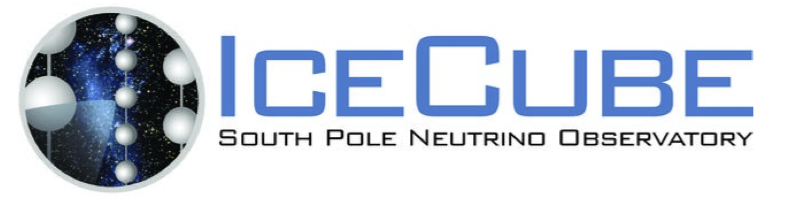
\includegraphics[height=1cm]{img/icecube-logo-side-text}}\hspace{0.3cm}
  % \raisebox{-0.1cm}{
\includegraphics[height=1cm]{img/DESY_logo_3C_web}}\hspace{0.5cm}
  \raisebox{-0.1cm}{
\includegraphics[height=1cm]{img/ecap}}\hspace{0.3cm}
  
\includegraphics[height=0.9cm]{img/logo-fau}
\fi}

\usepackage{graphicx}
\usepackage[font=footnotesize]{caption}
\usepackage{rotating}

\newcommand\image[1]{\includegraphics[width=\textwidth]{img/#1}}

\newcommand\fig[2]{
  \begin{figure}[htb]
    \begin{margincap}
      \centering
      \image{#1}
      \caption{#2}
    \end{margincap}
  \end{figure}
}

\usepackage{placeins} % implements \FloatBarrier
% Highlighted code listings, https://ctan.org/pkg/minted
%
% This requires pygments.
%
%     pip install Pygments
%     cd /Library/TeX/texbin
%     sudo ln -s `which pygmentize` pygmentize
%     sudo tlmgr install fvextra
%     sudo tlmgr update minted
%
\usepackage[outputdir=./build]{minted}

\setminted{
  tabsize=2, linenos, breaklines, autogobble, breakautoindent, frame=lines, framesep=2mm
}

\newenvironment{python}{\minted{python}}{\endminted}
\newcommand\pythoninput[1]{\inputminted{python}{#1}}

\setminted[python]{
  linenos=false,
  frame=none,
  fontsize=\footnotesize,
  escapeinside=||
}

\newenvironment{ccode}{\minted{c}}{\endminted}

\setminted[bash]{
  linenos=false
}

\newenvironment{bash}{\minted{bash}}{\endminted}
\usepackage{tabularx}
\usepackage{multirow}

% Tabellenanpassung
\newcommand{\oldarraystretch}{}
\newcolumntype{C}{>{\centering\arraybackslash}X}
\newcolumntype{R}{>{\raggedleft\arraybackslash}X}
\newcolumntype{L}{>{\raggedright\arraybackslash}X}

% vertical alignment
\renewcommand\tabularxcolumn[1]{m{#1}}


\newenvironment{tabelle}[1]%
{%
\renewcommand{\oldarraystretch}{\arraystretch}
  \renewcommand{\arraystretch}{1.5} % Tabellenabstände vergrößern
  \noindent\tabularx{\textwidth}{#1}
}{%
  \endtabularx
  \renewcommand{\arraystretch}{\oldarraystretch}
}

\usepackage{pgfshade}
\usetheme{Warsaw}
\setbeamercovered{transparent}
\usecolortheme{seahorse}

\beamertemplatenavigationsymbolsempty

\setbeamertemplate{footline}[author, title, frame number]

\newcommand{\vtiny}{\fontsize{6}{1}\selectfont}
\usepackage[absolute,overlay]{textpos}

\newcommand{\zitat}[2]{
  \textit{\frqq#1 \flqq}\\
  \begin{flushright}
    -- #2
  \end{flushright}
}
\newcommand{\source}[1]{
  \begin{textblock*}{\linewidth}(1cm,.92\paperheight)
    \vtiny Source: #1
  \end{textblock*}
}
\newcommand{\symbole}[1]{
  \begin{textblock*}{\linewidth}(1cm,.79\paperheight)
    \parbox{0.75\linewidth}{\vtiny #1}
  \end{textblock*}
}
\newcommand{\name}[1]{
  \textsc{#1}
}

\newcommand\follows{\item[$\rightarrow$]}

\setminted[bash]{
  linenos=false,
  fontsize=\scriptsize,
  baselinestretch=1
}

\newenvironment{smallbash}{\minted[fontsize=\tiny]{bash}}{\endminted}

\newenvironment{sideimage}[1]
  {
    \vspace{6mm}
    \hspace*{-4mm}
    \minipage{0.5\textwidth}
      \includegraphics[width=\textwidth]{#1}
    \endminipage
    \hspace*{8mm}
    \minipage{0.5\textwidth}
  }
  {\endminipage}

\newcommand\her[1]{\textbf{#1}}

% http://ctan.math.illinois.edu/macros/latex/contrib/enumitem/enumitem.pdf
\usepackage{enumitem}
\usepackage{xcolor}
\setlist{parsep=6pt}
\setitemize{label=\textbullet}
\setdescription{labelindent=0pt,labelwidth=2.1cm,labelsep*=1em,leftmargin=!, font={\mdseries\sffamily\color{blue}}}

% Slide number in footer
\newcommand*\oldmacro{}%
\let\oldmacro\insertshorttitle%
\renewcommand*\insertshorttitle{%
   \oldmacro\hfill%
   %\insertframenumber\,/\,\inserttotalframenumber}
   \insertframenumber}

% Logo in header
% https://tex.stackexchange.com/a/347635/70789
\makeatletter
\setbeamertemplate{headline}
{%
  \leavevmode%
  \@tempdimb=2.4375ex%
  \ifnum\beamer@subsectionmax<\beamer@sectionmax%
    \multiply\@tempdimb by\beamer@sectionmax%
  \else%
    \multiply\@tempdimb by\beamer@subsectionmax%
  \fi%
  \ifdim\@tempdimb>0pt%
    \advance\@tempdimb by 1.825ex%
    \begin{beamercolorbox}[wd=.5\paperwidth,ht=\@tempdimb]{section in head/foot}%
      \vbox to\@tempdimb{\vfil\insertsectionnavigation{.5\paperwidth}\vfil}%
    \end{beamercolorbox}%
    \begin{beamercolorbox}[wd=.5\paperwidth,ht=\@tempdimb]{subsection in head/foot}%
      \vbox to\@tempdimb{\vfil\insertsubsectionnavigation{.3\paperwidth}\vfil}%
      \hfill
      \unless\ifplacelogo % If the main logo is not shown, use the header logo
        \raisebox{0.18\headheight}{
\includegraphics[height=0.7\headheight]{img/icecube-sm}}
        \raisebox{0.3\headheight}{
\includegraphics[height=0.6\headheight]{img/ecap-sm}}
      \fi
    \end{beamercolorbox}%
  \fi%
}
\makeatother
\usepackage[T1]{fontenc}
\usepackage[utf8]{inputenc}
\usepackage{xspace}

\newcommand\unit[1]{\text{\,#1}\xspace}
\newcommand\m{\unit{m}}
\newcommand\cm{\unit{cm}}
\newcommand\mm{\unit{mm}}


% Markierungen mit `\todo{foo}`, `\mref{schiller}`, `\frage{foo}` einfügen.

\usepackage{color}

% Markierung einfügen (Kommentar während der Bearbeitung) % Parameter: Art, Kommentar
\newcommand{\markierung}[2]{
        \textcolor{red}{\textbf{#1:} #2} \\
}

\newcommand{\todo}[1]{\markierung{To do}{#1}} % ToDo-Kommentar einfügen, Parameter: Kommentar
\newcommand{\mref}[1]{\markierung{Verweis einfügen}{#1}} % Fehlenden Verweis markieren, Parameter: Kommentar
\newcommand\frage[1]{\markierung{Frage}{#1}} % Frage


\newcommand\done{\checkmark\xspace}
\newcommand\inprogress{$\Rightarrow$\xspace}
\newcommand\tobedone{$\square$\xspace}

%\includeonly{}

\begin{document}

% Warning: Do not indent \frame statements.
% This can lead to "Fatal error occurred, no output PDF file produced!"
% https://tex.stackexchange.com/a/225582/70789

\frame{\titlepage}

\placelogofalse

% \section{Introduction}
\begin{frame}{Resources}
  \begin{center}
    Usage examples can be found on github: \\ \vspace{0.3cm}
    \url{https://github.com/fiedl/hole-ice-study}
  \end{center}
\end{frame}

\begin{frame}{Contents}
  %\tableofcontents[hideallsubsections,sections=2-6]
  \tableofcontents[subsectionstyle=show]
\end{frame}

% %  %!TEX TS-program = ../make.zsh

\begin{frame}{Introduction: IceCube Detector}
  \centering
  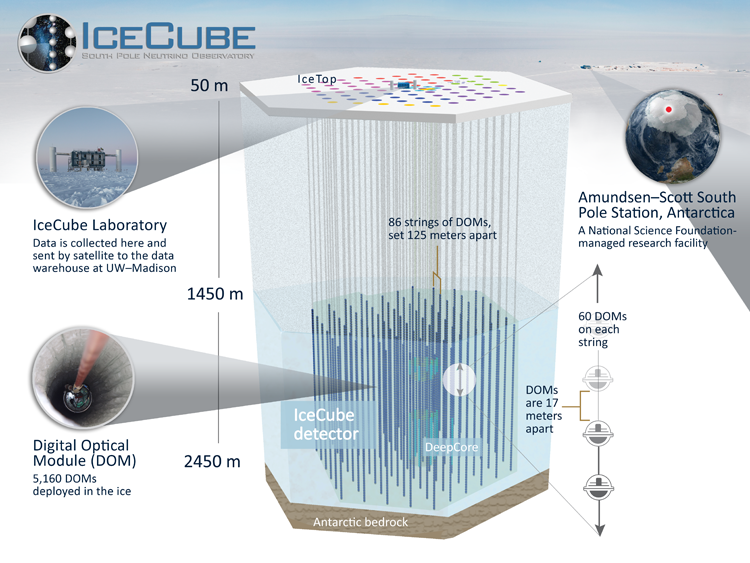
\includegraphics[height=0.9\textheight]{img/icecube_detector_sm}

  \tiny{Image source: \url{https://icecube.wisc.edu/icecube/static/science/images/icecube_detector_sm.png}}
\end{frame}
\begin{frame}{Motivation and Scope}
\begin{itemize}

  \item No hole-ice simulation included in clsim, yet
    \note[item]{
      clsim approximates hole ice using a convolution function for the angular acception.
      \item e.g. photons hitting a dom from below are made more unlikely to be detected.
      \item but no actual simulation of the changed ice properties.
    }
    \begin{itemize}
      \follows No asymmetries possible, e.g. DOM position relative to hole ice
      \note[item]{i.e. we can't have asymmetries like shifted DOM positions relative to the hole ice.}
    \end{itemize}

  \item Master thesis (ending Aug 2018)
    \note[item]{that's why I'm trying to implement propagation through cylinders with changed ice properties in clsim.}

\end{itemize}
\end{frame}

%   \include{text/how_does_it_look_like}
%!TEX TS-program = ../make.zsh

\begin{frame}{Contents}

  %\tableofcontents[hideallsubsections,sections=2-6]
  \tableofcontents[subsectionstyle=show]

  % Reminder: \url{https://docushare.icecube.wisc.edu/dsweb/View/Collection-15039}

\end{frame}

%\note[itemize]{
%  \item In this presentation, I'll show you what I've been working on
%  \item some examples with images and plots
%  \item point out some features that will be possible with this tool
%}

% 
% %!TEX TS-program = ../make.zsh

\begin{frame}[fragile]{Approach A (naive)}

  \begin{columns}
    \begin{column}{0.5\textwidth}
      \image{distance-correction}
    \end{column}
    \begin{column}{0.5\textwidth}
      \begin{itemize}
        \item \her{Minimal extension} to existing kernel
        \item Hole ice as \her{correction for each scattering step}
        \item Pros:
        \begin{itemize}
          \item Small surface area of implementation
          \item Standard \alert{clsim (well-tested) almost untouched}
          \item Very testable using unit tests
        \end{itemize}
        \item Cons:
        \begin{itemize}
          \item Hole-ice \alert{properties relative} to bulk ice
          \item Does \alert{not work with nested} cylinders
        \end{itemize}
      \end{itemize}
    \end{column}
  \end{columns}

  \source{https://github.com/fiedl/hole-ice-study/issues/45}

\end{frame}

\begin{frame}[fragile]{Approach B (the one to go)}

  \begin{columns}
    \begin{column}{0.5\textwidth}
      \image{how-does-it-work-004}
    \end{column}
    \begin{column}{0.5\textwidth}
      \begin{itemize}
        \item Treat hole ice and cables as \alert{media with ice optical properties}
        \item Generalize ice-layer algorithm
        \item Pros:
        \begin{itemize}
          \item Supports \alert{nested cylinders} and \alert{cables}
        \end{itemize}
        \item Cons:
        \begin{itemize}
          \item Needed to \alert{rewrite} some of the existing propagation kernel
          \item i.e. needed lots of \alert{statistical cross checks} to make sure everything works
        \end{itemize}
      \end{itemize}
    \end{column}
  \end{columns}

  \source{https://github.com/fiedl/hole-ice-study/issues/45}

\end{frame}


% 
\section{What can it do: Examples of Application}
\subsection{Vary drill-hole ice properties}
  \include{text/short_scattering_example}
\subsection{Realistic geometry}
  %!TEX TS-program = ../make.zsh

\begin{frame}[fragile]{Realistic simulation scenario} % Nested shifted cylinders and cable}

  \begin{columns}
    \begin{column}{0.6\textwidth}

      \image{cable-inside-shifted-bc-steamshovel}

    \end{column}
    \begin{column}{0.4\textwidth}

      \begin{itemize}
        \item DOM: radius 16.5\cm, shifted by 12.0\cm against the center of the bore hole
        \item bubble column: radius 8.0\cm
        \item drill-hole column: radius 30.0\cm
        \item cable: radius 3.0\cm, placed next to the DOM, partially within the bubble column
      \end{itemize}

      \vspace{1cm}
      \vtiny{See also: \url{https://github.com/fiedl/hole-ice-study/issues/110}}
    \end{column}
  \end{columns}

\end{frame}

%\subsection{POCAM Study}
%  \include{text/pocam}
%\subsection{Flasher Scan}
%%  %!TEX TS-program = ../make.zsh

\begin{frame}{Flasher-simulation example}

  Calibration: Find out the properties of the hole ice by comparing simulations with differnt properties to data of IceCube's LED-flasher-calibration system.\\

  \centering
  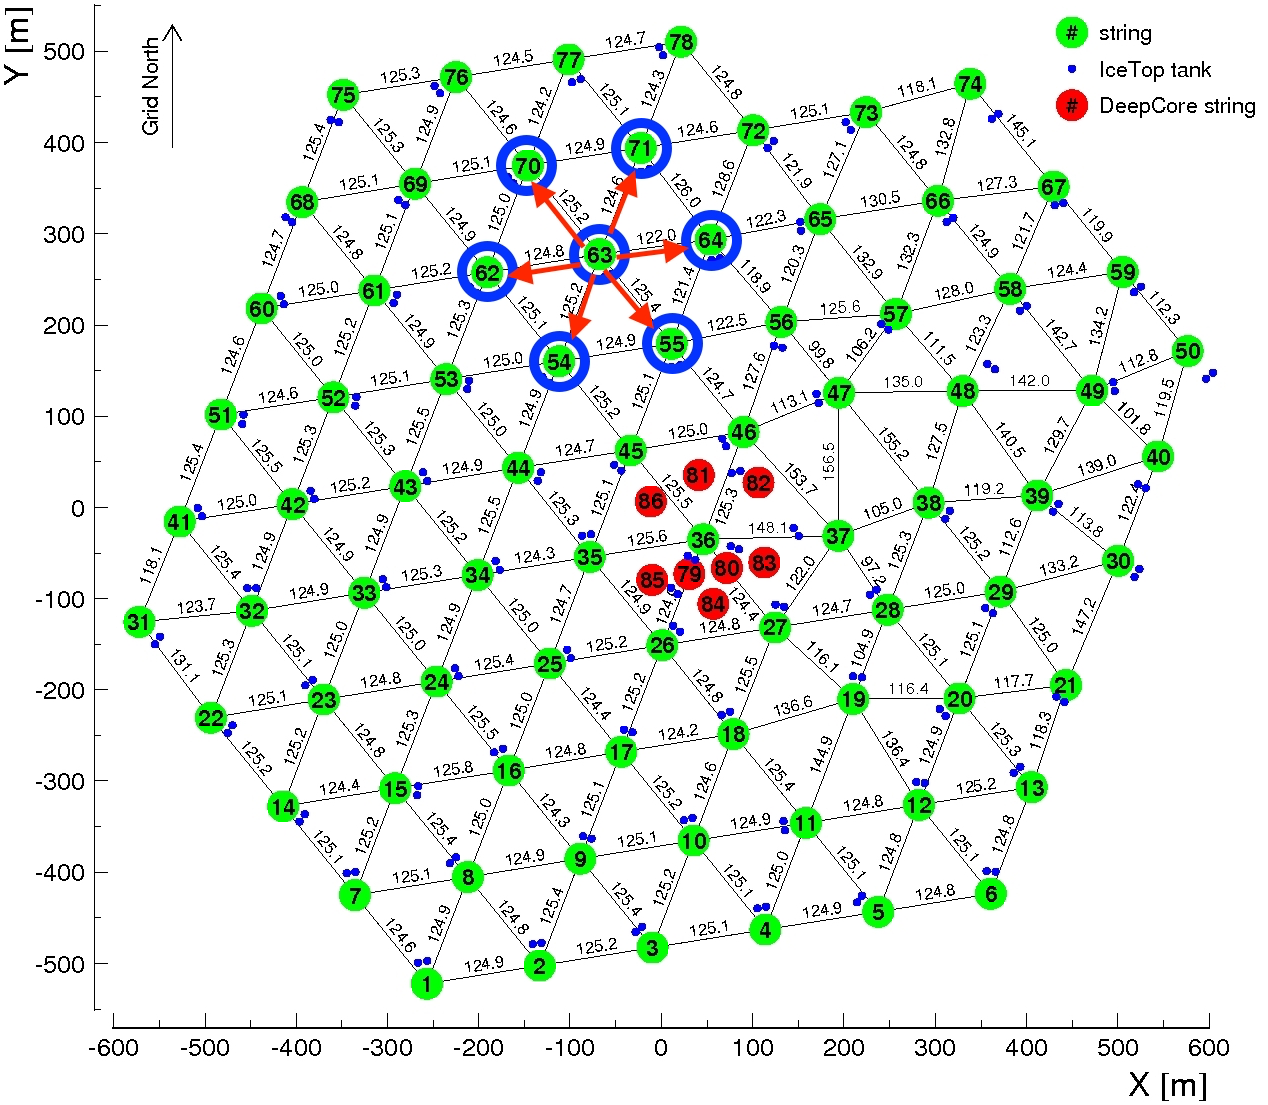
\includegraphics[height=0.35\textheight]{img/flasher-scenario}\hspace{1.2cm}
  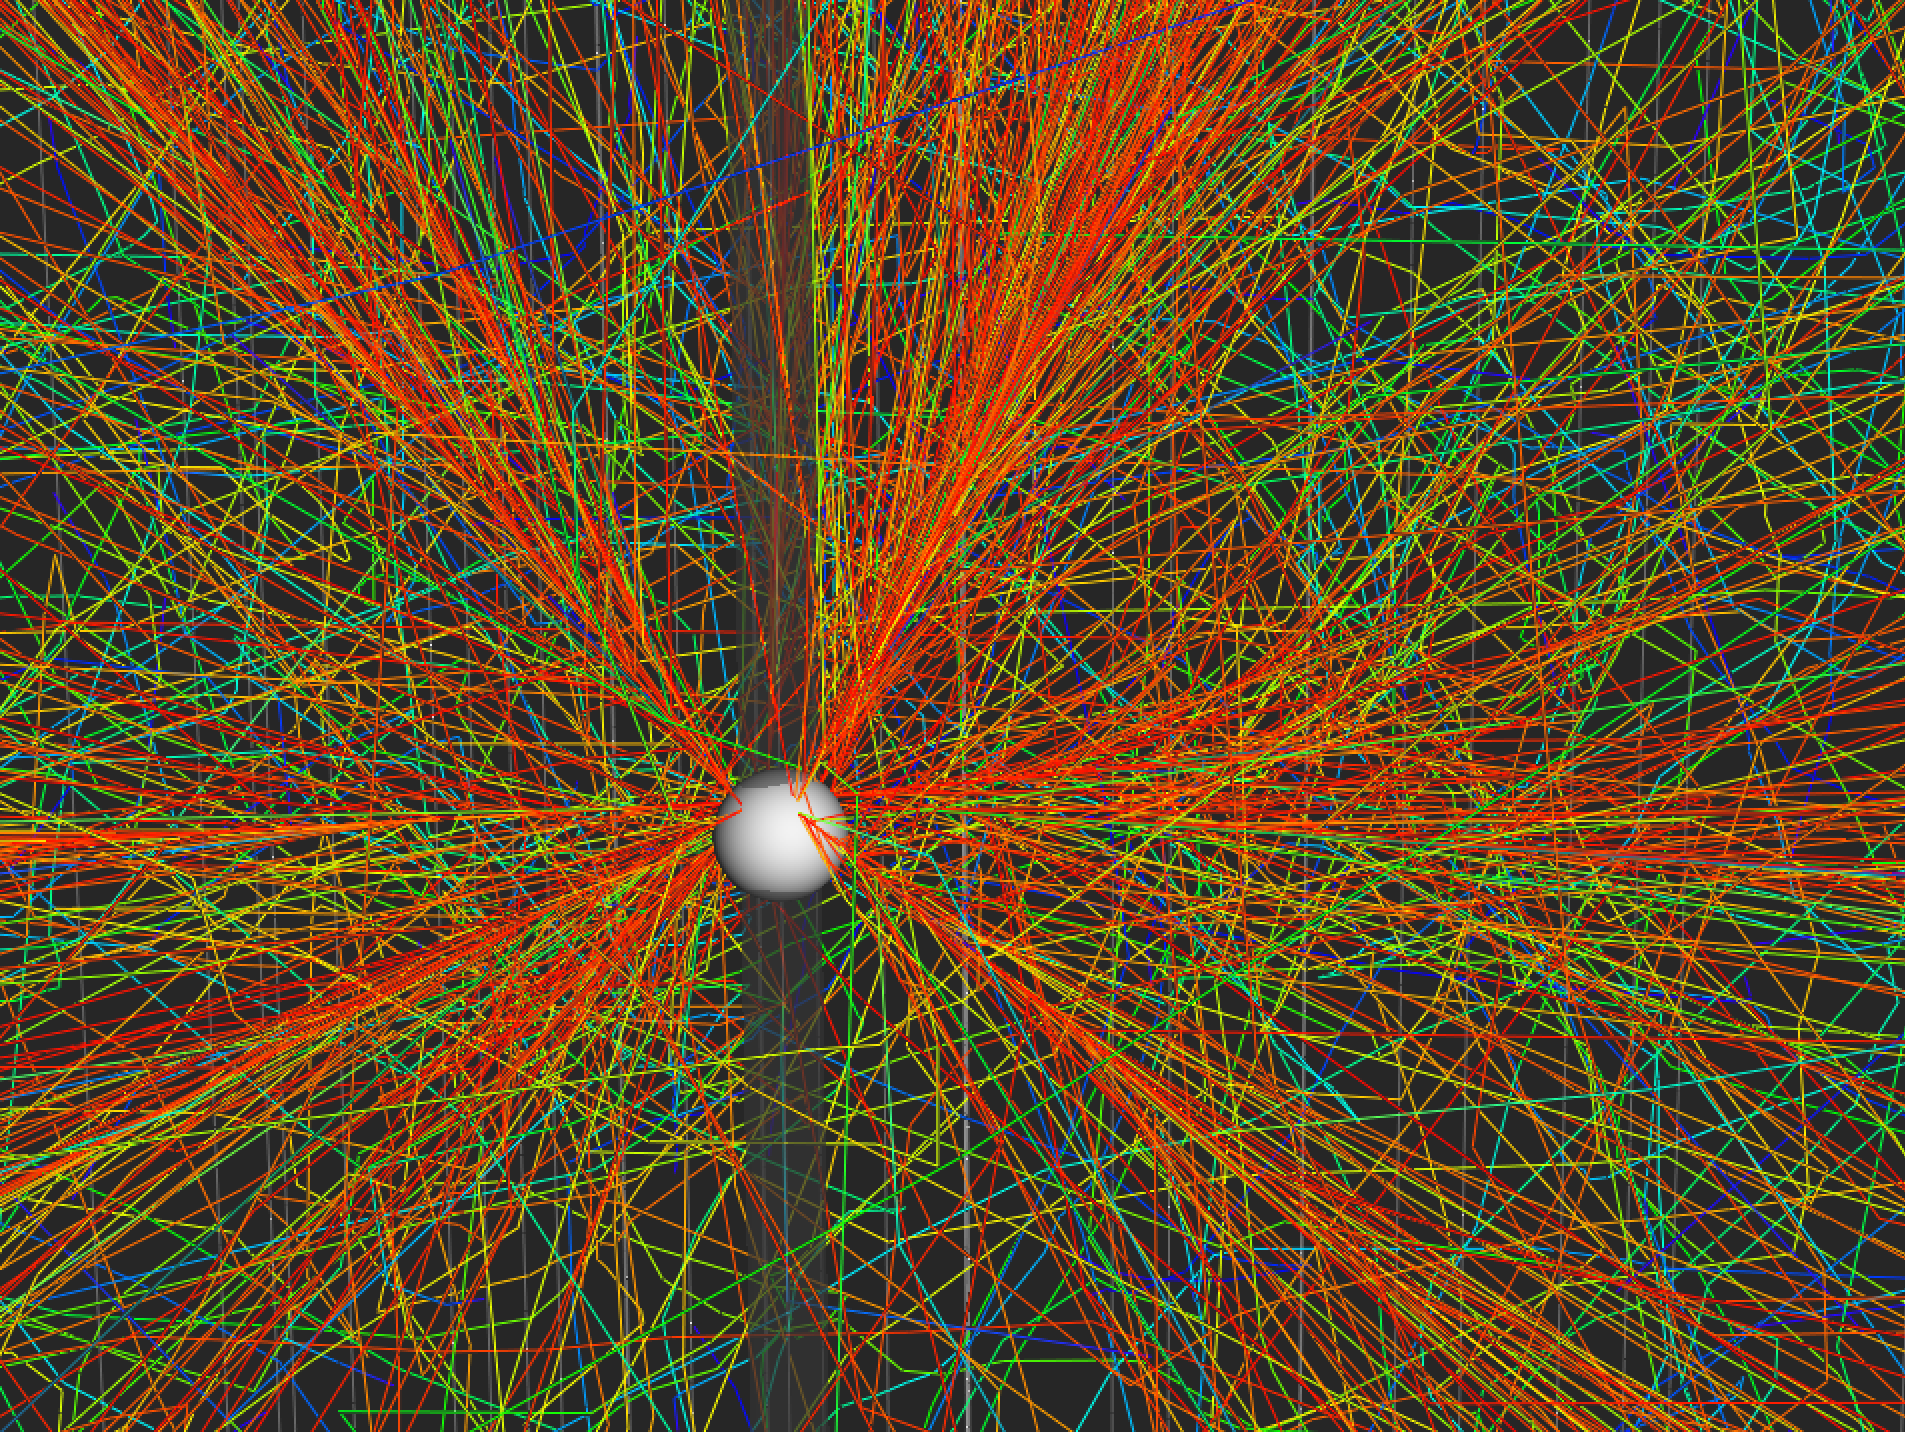
\includegraphics[height=0.35\textheight]{img/flasher-steamshovel-sending}

  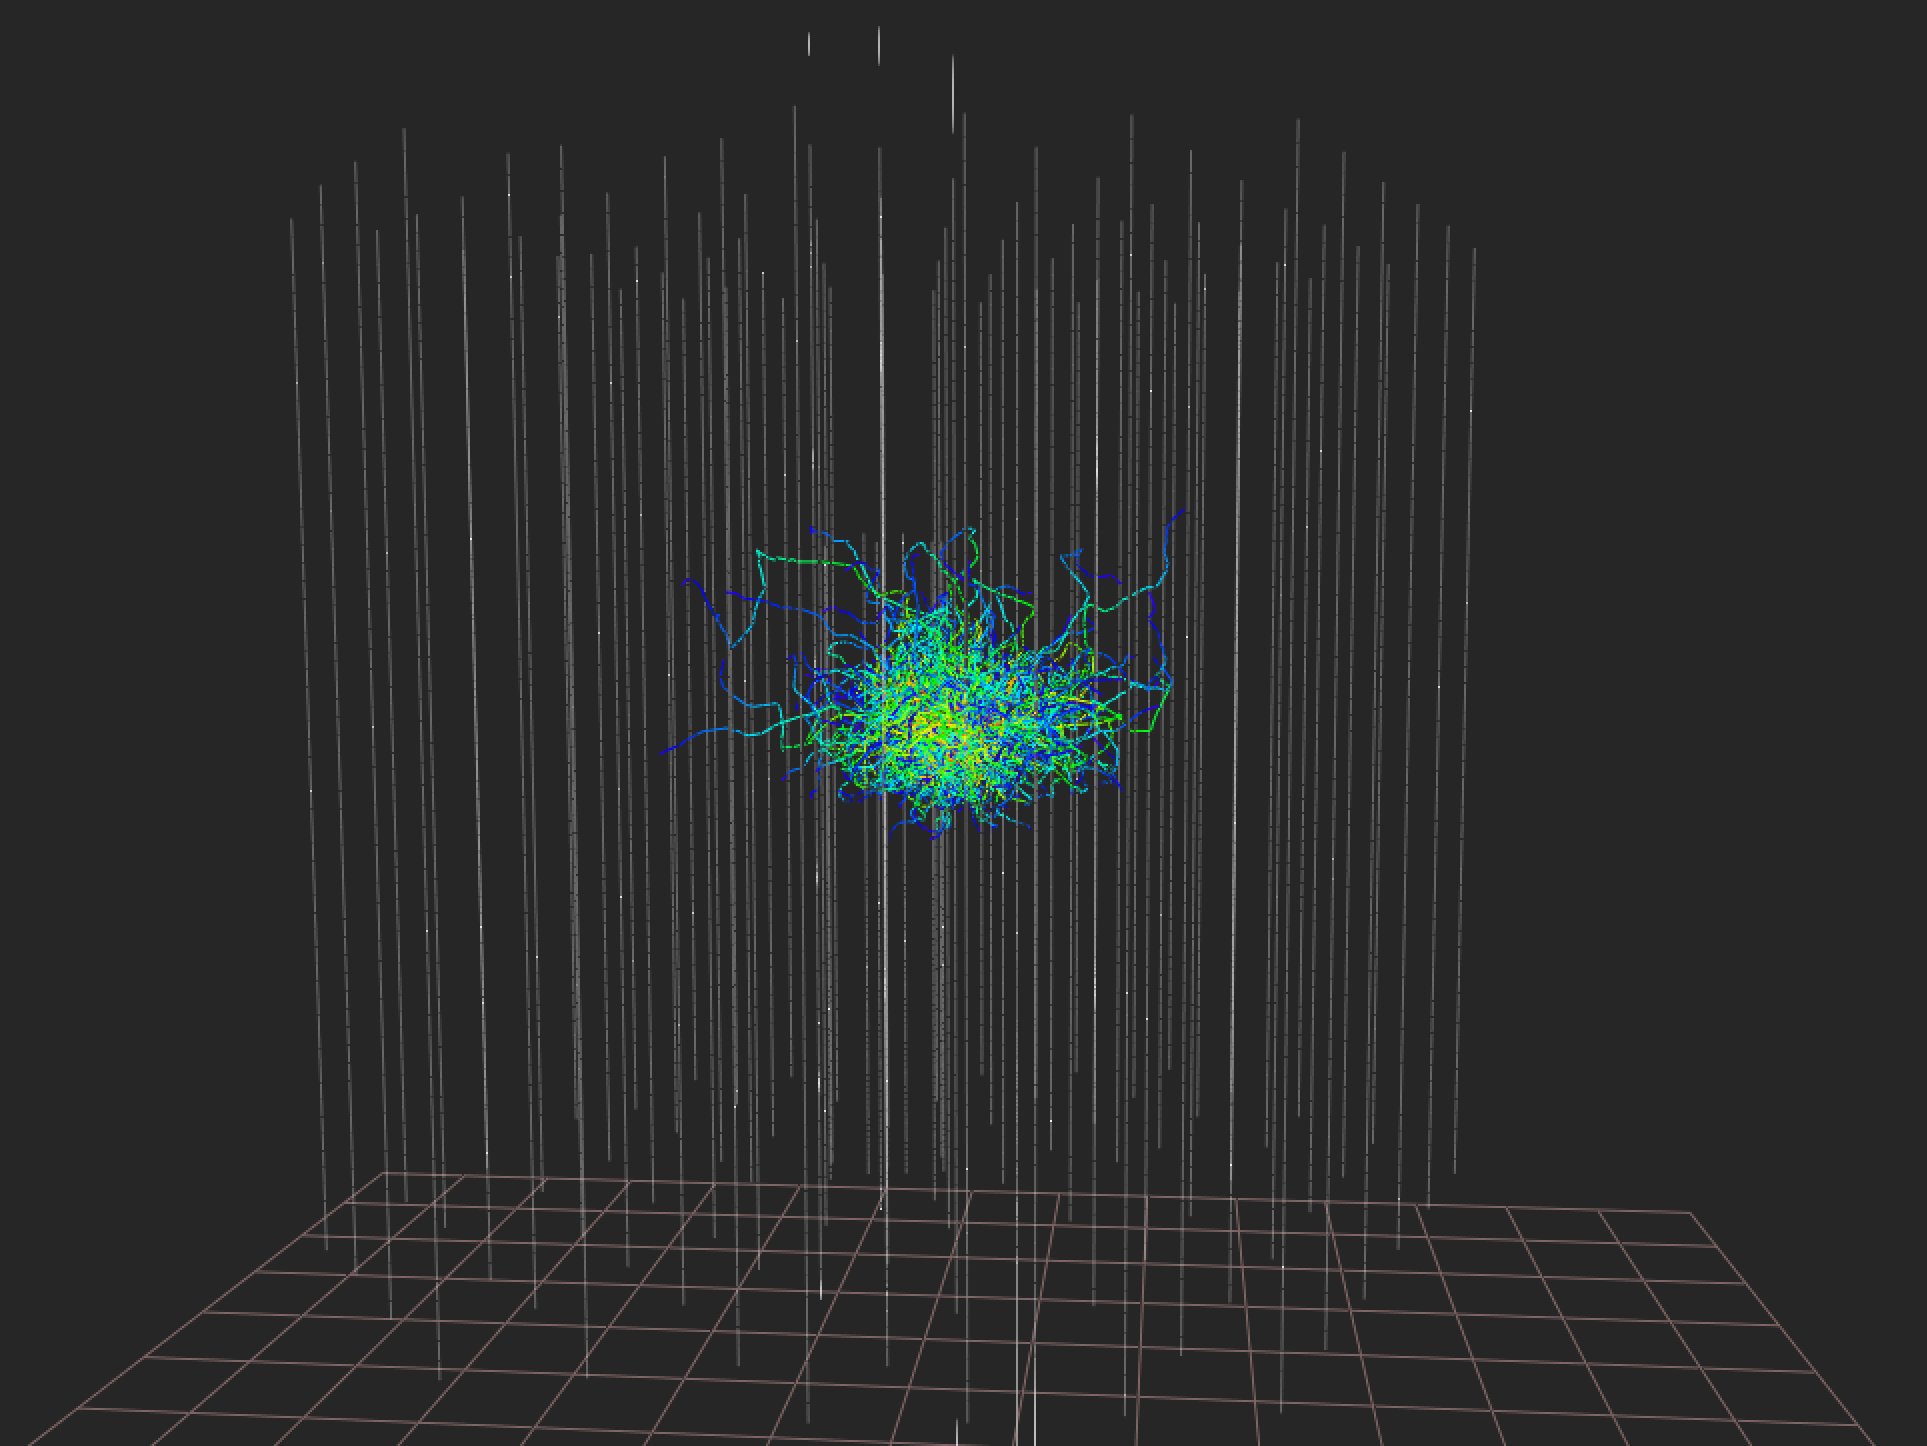
\includegraphics[height=0.35\textheight]{img/flasher-steamshovel-total}\hspace{3mm}
  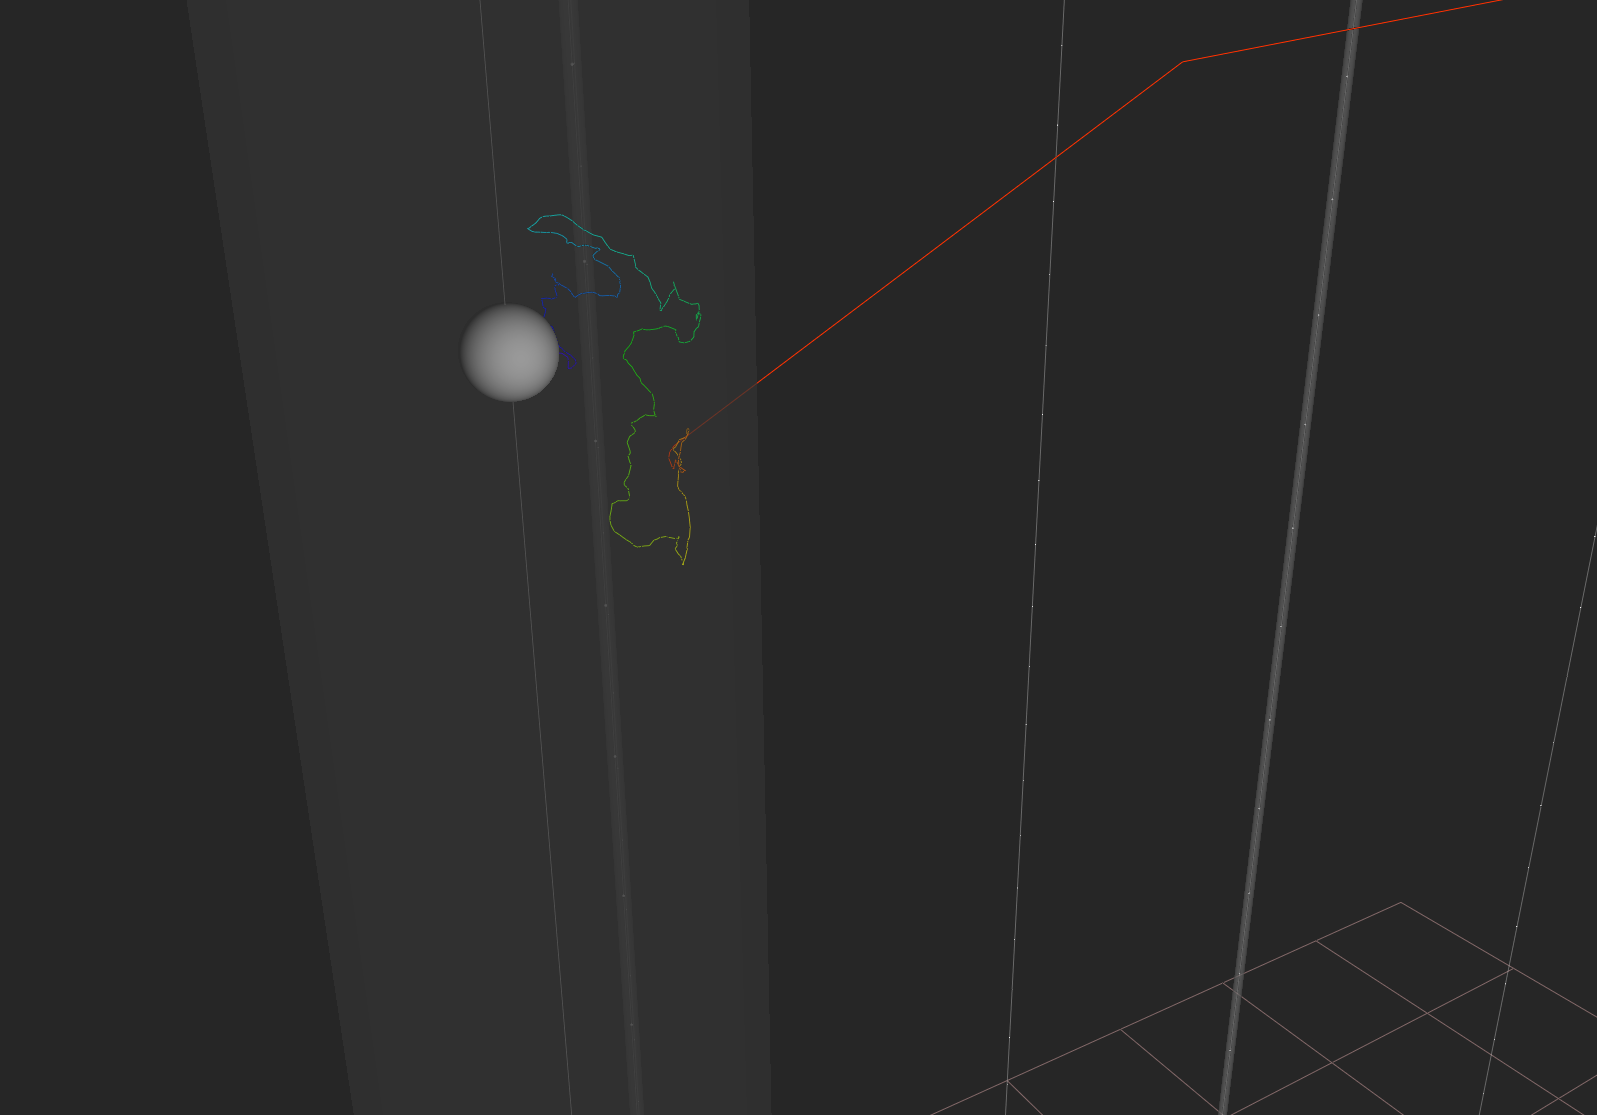
\includegraphics[height=0.35\textheight]{img/flasher-steamshovel-single-received-photon}

  \tiny{See \url{https://github.com/fiedl/hole-ice-study/issues/107}}

\end{frame}

%  %!TEX TS-program = ../make.zsh

\begin{frame}[fragile]{Early results: Example scan for best hole-ice parameters based on calibration data}
  \begin{column}{0.5\textwidth}
    \image{flasher-scenario-light}
  \end{column}
  \begin{column}{0.5\textwidth}
    \image{flasher-contours-59}
  \end{column}

  \source{\url{https://github.com/fiedl/hole-ice-study/issues/59}. Image based on \url{https://wiki.icecube.wisc.edu/index.php/File:Distances.i86.jpg}.}
\end{frame}

% \begin{frame}[fragile]{Flasher parameter scan vs. SpiceHD scan}
%   \begin{column}{0.5\textwidth}
%     SpiceHD with ppc: \medskip
%
%     \image{flasher-contours-martin}
%
%     DOM positions are fit parameters.
%   \end{column}
%   \begin{column}{0.5\textwidth}
%     clsim with direct hole ice: \medskip
%
%     \image{flasher-same-color-axis-as-spicehd}
%
%     All DOMs perfectly centered within hole ice.
%   \end{column}
%
%   \bigskip
%   Mind systematics: DOM displacement does account for the observed scattering-length factor $\frac{1}{3}$ for the hole-ice radius of 1.8 dom radii (right-hand side of the plot).
%
%   \source{\url{https://github.com/fiedl/hole-ice-study/issues/106}. }
% \end{frame}
%\subsection{DOM Types}
%  \include{text/dom_types}

% \section{How does it work?}
%   \include{text/how_does_algorithm_b_work}

\section{How can I use it?}
  %!TEX TS-program = ../make.zsh

\begin{frame}[t,fragile]{How can I configure the simulation?}
  \begin{column}[t]{0.37\textwidth}
    \begin{overlayarea}{\textwidth}{\textheight}
      \only<1>{\image{config-example-steamshovel-0}}
      \only<2>{\image{config-example-steamshovel-1}}
      \only<3>{\image{config-example-steamshovel-2}}
      \only<4-5>{\image{config-example-steamshovel-3}}
      \only<6>{\image{config-example-steamshovel-4}}
      
      \vspace*{3cm}
      README: \url{https://github.com/fiedl/hole-ice-scripts}
    \end{overlayarea}
  \end{column}
  \begin{column}[t]{0.6\textwidth}
    \vspace*{-14cm}
    \begin{python}
      from icecube.simclasses import I3CLSimMediumCylinder, I3CLSimMediumCylinderSeries
    \end{python}
    \begin{onlyenv}<2->
      \begin{python}
        drill_hole_cylinder = I3CLSimMediumCylinder()
        drill_hole_cylinder.x = -256.14 + (0.30 - 0.16510) # m
        drill_hole_cylinder.y = -521.08 # m
        drill_hole_cylinder.radius = 0.30 # m
        drill_hole_cylinder.scattering_length = 0.004 # m
      \end{python}
    \end{onlyenv}

    \begin{onlyenv}<3->
      \begin{python}
        bubble_column_cylinder = I3CLSimMediumCylinder()
        bubble_column_cylinder.x = -256.14 + (0.30 - 0.16510) # m
        bubble_column_cylinder.y = -521.08 # m
        bubble_column_cylinder.radius = 0.10 # m
        bubble_column_cylinder.scattering_length = 0.001 # m
      \end{python}
    \end{onlyenv}

    \begin{onlyenv}<4->
      \begin{python}
        cable_cylinder = I3CLSimMediumCylinder()
        cable_cylinder.x = -256.14 + (0.16510 + 0.03) # m
        cable_cylinder.y = -521.08 # m
        cable_cylinder.top = 496.03 + 0.5 # m
        cable_cylinder.bottom = 496.03 - 0.5 # m
        cable_cylinder.radius = 0.03 # m
        cable_cylinder.absorption_length = 0.0 # m
      \end{python}
    \end{onlyenv}
    
    \begin{onlyenv}<5->
      \begin{python}
        cylinders = I3CLSimMediumCylinderSeries([drill_hole_cylinder, bubble_column_cylinder, cable_cylinder])
        geometry_frame.Put("I3CLSimMediumCylinders", cylinders)
      \end{python}
    \end{onlyenv}
    
  \end{column}
\end{frame}

\begin{frame}[t,fragile]{How can I configure the simulation? [WIP]}
  \begin{column}[t]{0.37\textwidth}
    \image{config-example-steamshovel-5}
    
    \vspace{0.5cm}
    \only<3>{\image{dom_types_with_shapes}}

  \end{column}
  \begin{column}[t]{0.6\textwidth}
    \vspace*{-5cm}
    
    \begin{onlyenv}<1>
      \begin{python}
        # work in progress:
        
        upper_pmt = I3CLSimMediumSphere()
        upper_pmt.absorption_length = 0 # m
        upper_pmt.detection_probability = 0.2
        # ...
        
        lower_pmt = I3CLSimMediumSphere()
        lower_pmt.absorption_length = 0 # m
        lower_pmt.detection_probability = 0.2
        # ...
        
        cylinder = I3CLSimMediumCylinder()
        cylinder..absorption_length = 0 # m
        # ...
        
        shapes = I3CLSimMediumShapeSeries([upper_pmt, lower_pmt, cylinder])
        geometry_frame.Put("I3CLSimMediumShapes", shapes)
      \end{python}
    \end{onlyenv}
    
    \begin{onlyenv}<2->
      \begin{python}
        # work in progress:
        
        upper_pmt = I3CLSimMediumSphere()
        upper_pmt.absorption_length = 0 # m
        upper_pmt.detection_probability = 0.2
        # ...
        
        lower_pmt = |\colorbox{yellow}{I3CLSimMediumSphere()}|
        lower_pmt.absorption_length = 0 # m
        lower_pmt.|\colorbox{yellow}{detection\_probability}| = 0.2
        # ...
        
        cylinder = |\colorbox{yellow}{I3CLSimMediumCylinder()}|
        cylinder..absorption_length = 0 # m
        # ...
        
        shapes = I3CLSimMediumShapeSeries([upper_pmt, lower_pmt, cylinder])
        geometry_frame.Put("I3CLSimMediumShapes", shapes)
      \end{python}
    \end{onlyenv}
    
  \end{column}
\end{frame}



\section{Performance}
  %!TEX TS-program = ../make.zsh

\begin{frame}[fragile]{Performance}
  \begin{itemize}
    \item Performance per scattering step is the same as with standard clsim
    \item However, for smaller scattering lengths, the number of scattering steps increases
    \follows \her{Longer simulation time with hole ice}
  \end{itemize}

  \source{\url{https://github.com/fiedl/hole-ice-study/issues/69}}
\end{frame}

\section{Where does this tool fit in?}
  \include{text/where_does_it_fit_in}
  %%!TEX TS-program = ../make.zsh

\begin{frame}[fragile]{Where does this tool fit in?}

  Apply this to Upgrade/Gen2 problems?
  \vspace{1cm}

  \begin{itemize}
    \item Strength: Propagation through \alert{different media with sharp boundaries}
    \item \alert{Arbitrary shapes} as long as we can calcualte the intersection points with the photon ray
    \item Interactions: \textit{Scatter}, \textit{Absorb}, \alert{plus: \textit{Detect}}
    \item Performance:
    \begin{itemize}
      \item When running the same scenario, simulation \her{performance} is the \her{same as before}. \checkmark
      \item When running scenarios with \her{more scattering, simulation time increases} accordingly as expected.
      \item In comparison to other tools, \alert{compromise} of \alert{performance} and \alert{level of detail}
    \end{itemize}
    
    \vspace{0.5cm}
    \item[$\Rightarrow$] Good for calibration and exploration, too slow for production
  \end{itemize}

\end{frame}


\section{Status}
  \include{text/status}

%\section{Results}
%  \include{text/results}

%\section{Outlook}
%%!TEX TS-program = ../make.zsh

\begin{frame}{Outlook: Next Steps}
  \begin{itemize}
    \item Bring the new hole-ice simulation into IceCube's main simulation framework
    %\item Study impact of hole ice on low-energy systematics
    \item Find best hole-ice parameters (radius, scattering length) with calibration data
    \item Provide new approximation for use with high-energy studies, where a direct simulation would be too expensive
    \item Study calibration scenarios for upcoming IceCube Upgrade
  \end{itemize}
\end{frame}

%!TEX TS-program = ../make.zsh

\placelogotrue
\begin{frame}{Thanks for your attention!}
  \begin{center}
    Any input you might have is welcome: \\ \vspace{0.3cm}

    \url{https://github.com/fiedl/hole-ice-study/issues} \\ \vspace{0.1cm}

    %Slack: \href{https://icecube-spno.slack.com/messages/@U092MBFU2}{\texttt{@fiedl}}
    sebastian.fiedlschuster@fau.de

    \vspace{1.5cm}

    \small{
      Video illustration of a simple example: \\
      \url{https://youtu.be/BhJ6F3B-I1s}
    }

  \end{center}
\end{frame}
\placelogofalse


\appendix
\section{Backup slides}

\subsection{Hole ice}
  \include{text/what_is_hole_ice}

\section{Photon-Propagation Algorithm}
  %!TEX TS-program = ../make.zsh

\begin{frame}[fragile]{How does it work?}

  \begin{columns}
    \begin{column}{0.5\textwidth}
      \begin{overlayarea}{\textwidth}{\textheight}
        \vspace*{2cm}
        \only<1>{\image{how-does-it-work-001}}
        \only<2>{\image{how-does-it-work-002}}
        \only<3>{\image{how-does-it-work-003}}
        \only<4>{\image{how-does-it-work-004}}
      \end{overlayarea}
    \end{column}
    \begin{column}{0.5\textwidth}

      \begin{itemize}
        \item Photon scattering points $A$ and $B$
        \item<1> \her{Naive algorithm}: Propagate photon small distance $\delta x$ in each simulation step and randomize whether the photon will scatter in this step (easy to implement local properties)
        \item<2> \her{Faster algorithm}: Randomize geometric distance to next scattering point and propagate from $A$ to $B$ in one simulation step
        \item<3> \her{Ice layers in clsim}: Randomize number of scattering lengths between $A$ and $B$ as budget and calculate geometric distance by spending the budget over the ice layers
        \item<4> \her{New: Hole ice} in clsim: Generalize budget algorithm to support cylinders (with distinct scattering and absorption lengths) in addition to ice layers.
      \end{itemize}

    \end{column}
  \end{columns}

\end{frame}
  \include{text/how_does_algorithm_b_work}

\subsection{Performance considerations}
  %!TEX TS-program = ../make.zsh

\begin{frame}[fragile]{Performance}

  Time measurement: Propagating $10^5$ photons on CPU

  \begin{columns}
    \begin{column}{0.6\textwidth}
      \image{performance-medium-changes}

      \begin{smallbash}
        $ICESIM/env-shell.sh
        cd $HOLE_ICE_STUDY/scripts/AngularAcceptance
        time ./run.rb --distance=1.0 --number-of-runs=1 --number-of-parallel-runs=1 --cpu --angle=45 --plane-wave --number-of-photons=1e5
      \end{smallbash}

    \end{column}
    \begin{column}{0.4\textwidth}
      \begin{itemize}
        \item Medium propagation features (hole ice, layers) have no measurable performance impact.
        \item Hole-ice-2017 and hole-ice-2018 algorithms have no measurable performance impact for scattering lengths comparable to bulk-ice scattering ($\lambda_s = 20\m$).
        \item Performance drop can be seen when lowering the scattering length, i.e. increasing the number of simulation steps ($\lambda_s = 3\mm$).
      \end{itemize}
    \end{column}
  \end{columns}

\source{https://github.com/fiedl/hole-ice-study/issues/49}

\end{frame}
  %!TEX TS-program = ../make.zsh

\begin{frame}[fragile]{Performance on GPU}
  \her{Performance of one simulation step} depends on optimizations: \\

  \image{profiling-paz4Eig6}

  \bigskip

  \her{Total performance} depends on number of scatters: \\

  Standard clsim with hole-ice approximation: 11 mins \\
  New algorithm, no hole ice: 10 mins \\
  New algorithm, about H2 hole ice: 15 mins % r = 36cm, esca = 1/10 bulk

  \source{\url{https://github.com/fiedl/hole-ice-study/issues/69}}

\end{frame}
  %!TEX TS-program = ../make.zsh

\begin{frame}[fragile]{Coordinates-vs-vectors bug}

  Scenario: Instant absorption. Top view.
  Mathematics of intersection calculations and starting conditions are the same in both figures.

  \begin{columns}
    \begin{column}{0.5\textwidth}

      Before: Treating coordinates as separate variables
      \image{coordinates-vs-vectors-bug-before}

    \end{column}
    \begin{column}{0.5\textwidth}

      After: Treating vectors as opencl-native vectors
      \image{coordinates-vs-vectors-bug-after}

    \end{column}
  \end{columns}

  \source{\url{https://github.com/fiedl/hole-ice-study/issues/28}}
\end{frame}

\subsection{Direct detection}
  %!TEX TS-program = ../make.zsh

\begin{frame}[fragile]{Direct detection}

  \begin{columns}
    \begin{column}{0.5\textwidth}

      \image{direct-detection}

    \end{column}
    \begin{column}{0.5\textwidth}

      \begin{itemize}
        \item The DOM looks downwards by design
        \item Currently, the hit position is not used when determining DOM acceptance, just the photon direction when hitting the DOM (\textit{DOM angular acceptance})
        \item Direct detection: Accept all hits below the waist band, reject all others
        \item Direct detection is easy with clsim
          \begin{itemize}
            \item Hit position is known and guaranteed to be on the DOM sphere
            \item Idea: Accept hits depending on $z$ of the hit position
            \item Patch is a couple of lines: \href{https://github.com/fiedl/clsim/commit/96a2e3fa1f9bb283b1b98f351e1a131b376a72b8}{fiedl/clsim@96a2e3f}
          \end{itemize}
        \item Still work to be done:
          \begin{itemize}
            \item Implement a switch for direct detection vs. DOM angular acceptance
                \tiny \url{https://github.com/fiedl/hole-ice-study/issues/32} \small
            \item Consider DOM orientation
                \tiny \url{https://github.com/fiedl/hole-ice-study/issues/53} \small
          \end{itemize}
      \end{itemize}


    \end{column}
  \end{columns}

  \source{Image: Martin Rongen, \textit{Status and future of SpiceHD & DARD}, 2017, Slide 17, \\ See also: \url{https://github.com/fiedl/hole-ice-study/issues/32}}
\end{frame}


\subsection{Angular acceptance}
  %!TEX TS-program = ../make.zsh

\begin{frame}[fragile]{Angular acceptance}

  For each angle $\eta$, shoot photons onto the DOM and count hits.

  \begin{columns}
    \begin{column}{0.5\textwidth}
      \image{angular-acceptance}
    \end{column}
    \begin{column}{0.5\textwidth}

      \only<1>{
        \begin{figure}
          \image{ice-paper-fig7}
          \caption*{Angular acceptance \textit{reference curves}. The nominal model is based on lab measurement, the hole ice curve on previous simulations.}
        \end{figure}
      }

      \begin{onlyenv}<2>
        \image{angular-acceptance-example-plane-waves}

        \begin{smallbash}
          $ICESIM/env-shell.sh; cd $HOLE_ICE_STUDY/scripts/AngularAcceptance
          ./run.rb --scattering-factor=0.1 --absorption-factor=1.0 --distance=1.0 --plane-wave --number-of-photons=1e5 --angles=0,10,20,30,32,45,60,75,90,105,120,135,148,160,170,180] --number-of-runs=2 --number-of-parallel-runs=2
          open results/current/plot_with_reference.png
        \end{smallbash}
      \end{onlyenv}
    \end{column}
  \end{columns}

  \source{Image: Martin Rongen, Calibration Call 2015-11-06, DARD Update, Slide 9 \\ Plot: \href{https://arxiv.org/abs/1301.5361}{Measurement of South Pole ice transparency with the IceCube LED calibration system}, 2013, figure 7. See also: \url{https://github.com/fiedl/hole-ice-study/issues/10}}

\end{frame}

\note[itemize]{
  \item One way to compare the new simulation to existing results, is to plot angular-acceptance curves.
  \item I.e. for each angle $\eta$, which is the angle between the starting direction of the photon and the column axis, shoot photons onto the DOM, propagate them in simulation and count hits.
  \item The current hole-ice approximations are convolutions onto the DOM angular acceptance.
  \item This is an example using the new hole-ice simulation with arbitrary ice parameters (data points) compared to the old reference curve (red).
}
  %!TEX TS-program = ../make.zsh

\begin{frame}[fragile]{Angular acceptance for different hole-ice parameters}
  \begin{column}{0.5\textwidth}
    Vary hole-ice scattering length: \medskip

    \image{angular-acceptance-vary-esca-83}
  \end{column}
  \begin{column}{0.5\textwidth}
    Vary hole-ice radius: \medskip

    \image{angular-acceptance-vary-radius-82}
  \end{column}

  Systematics: \\
  For direct detection + plane waves, increased number of photons for $\cos \eta < 0$. \\
  plane extent 1\m, starting distance 1\m \\
  non-perfect bulk-ice properties

\end{frame}

 % including systematics
  %!TEX TS-program = ../make.zsh

\begin{frame}{Angular acceptance: Sources and acceptance criteria}
  \begin{center}
    \only<1>{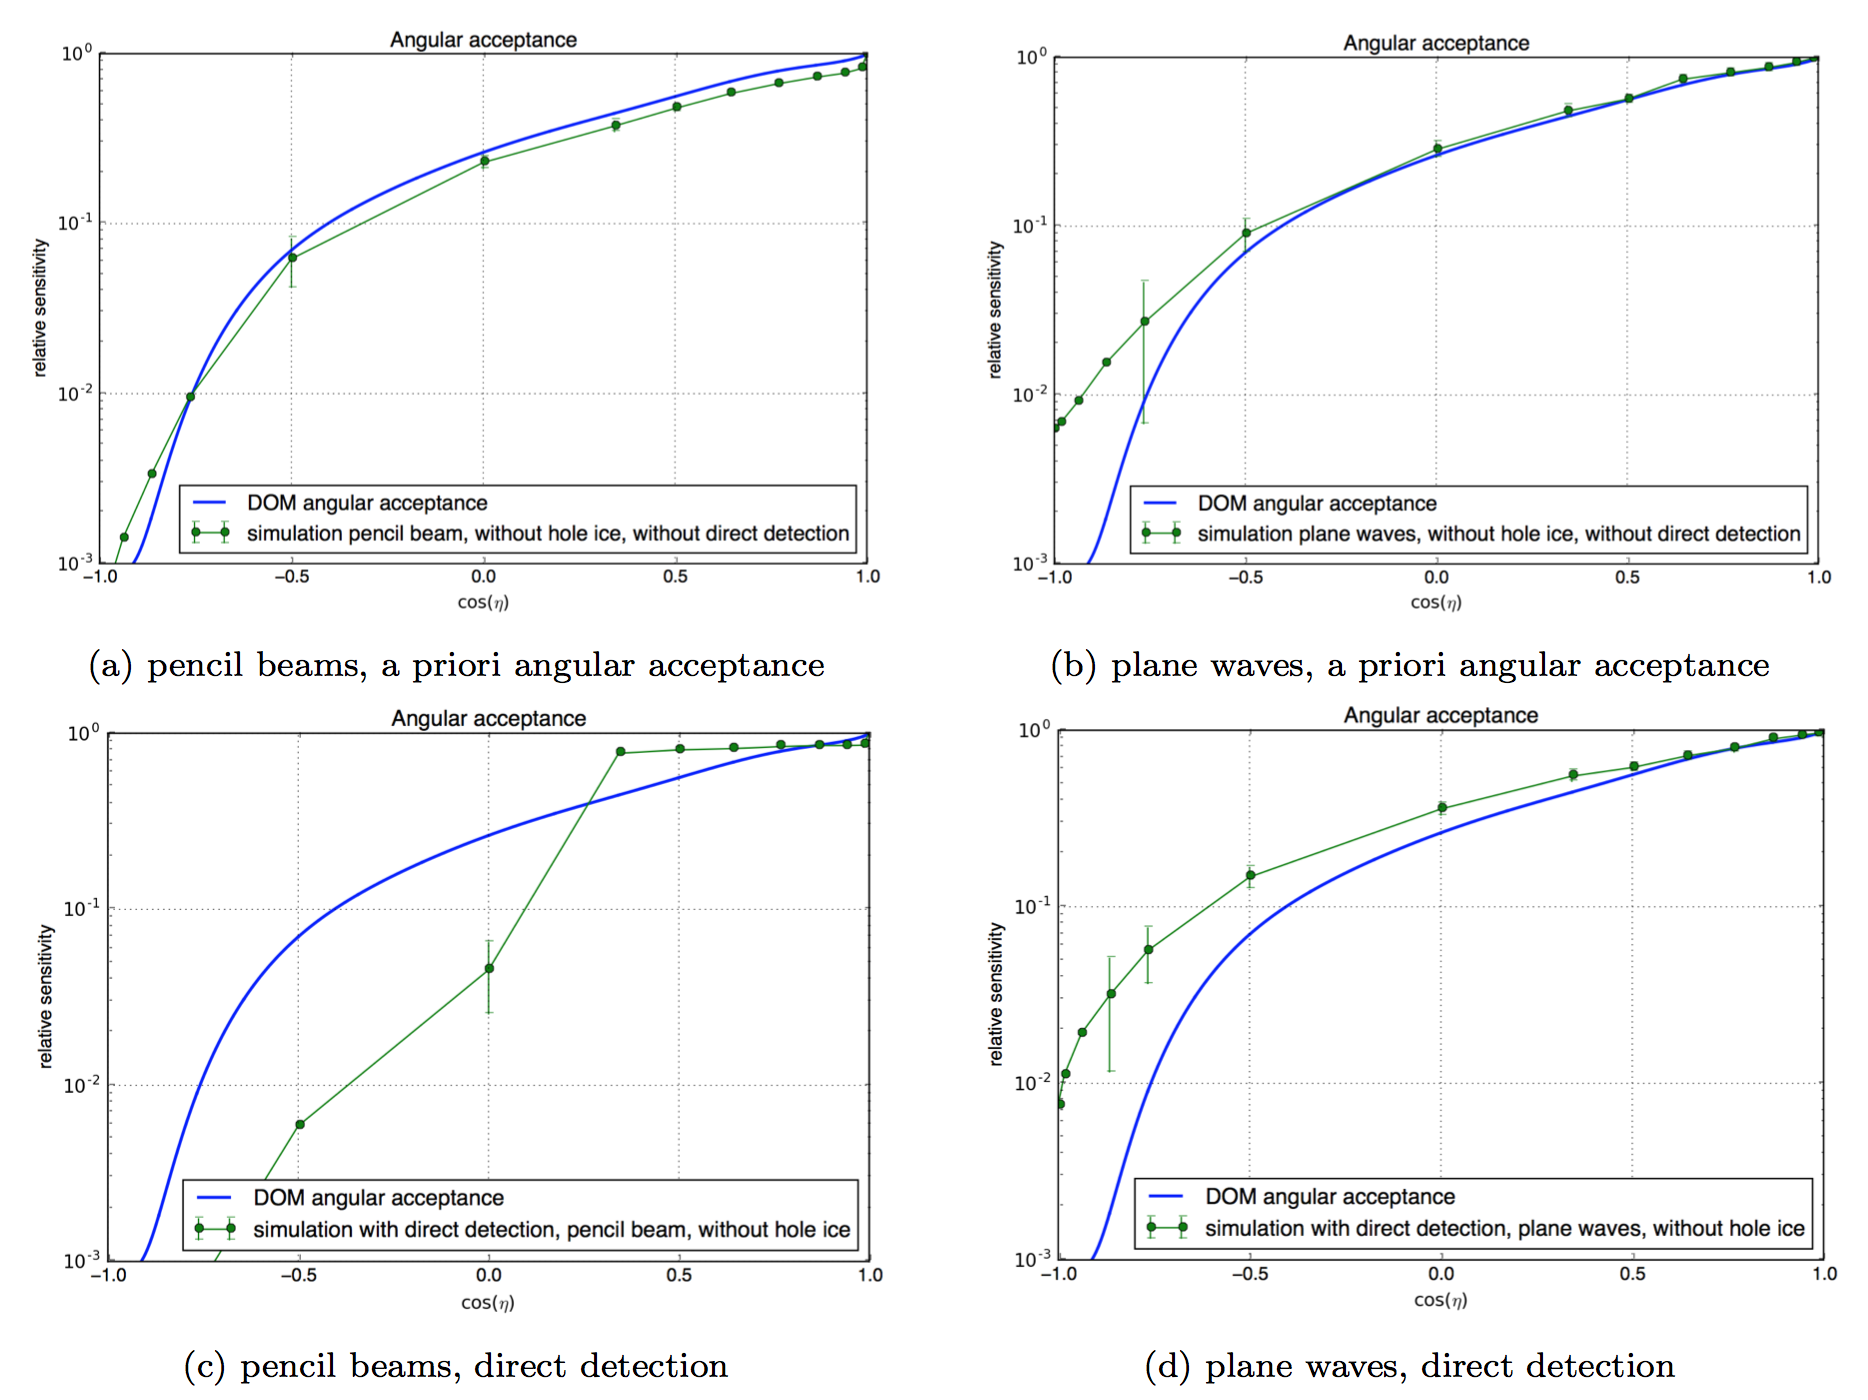
\includegraphics[width=0.7\textwidth]{img/angular-acceptance-methods}}
    \only<2>{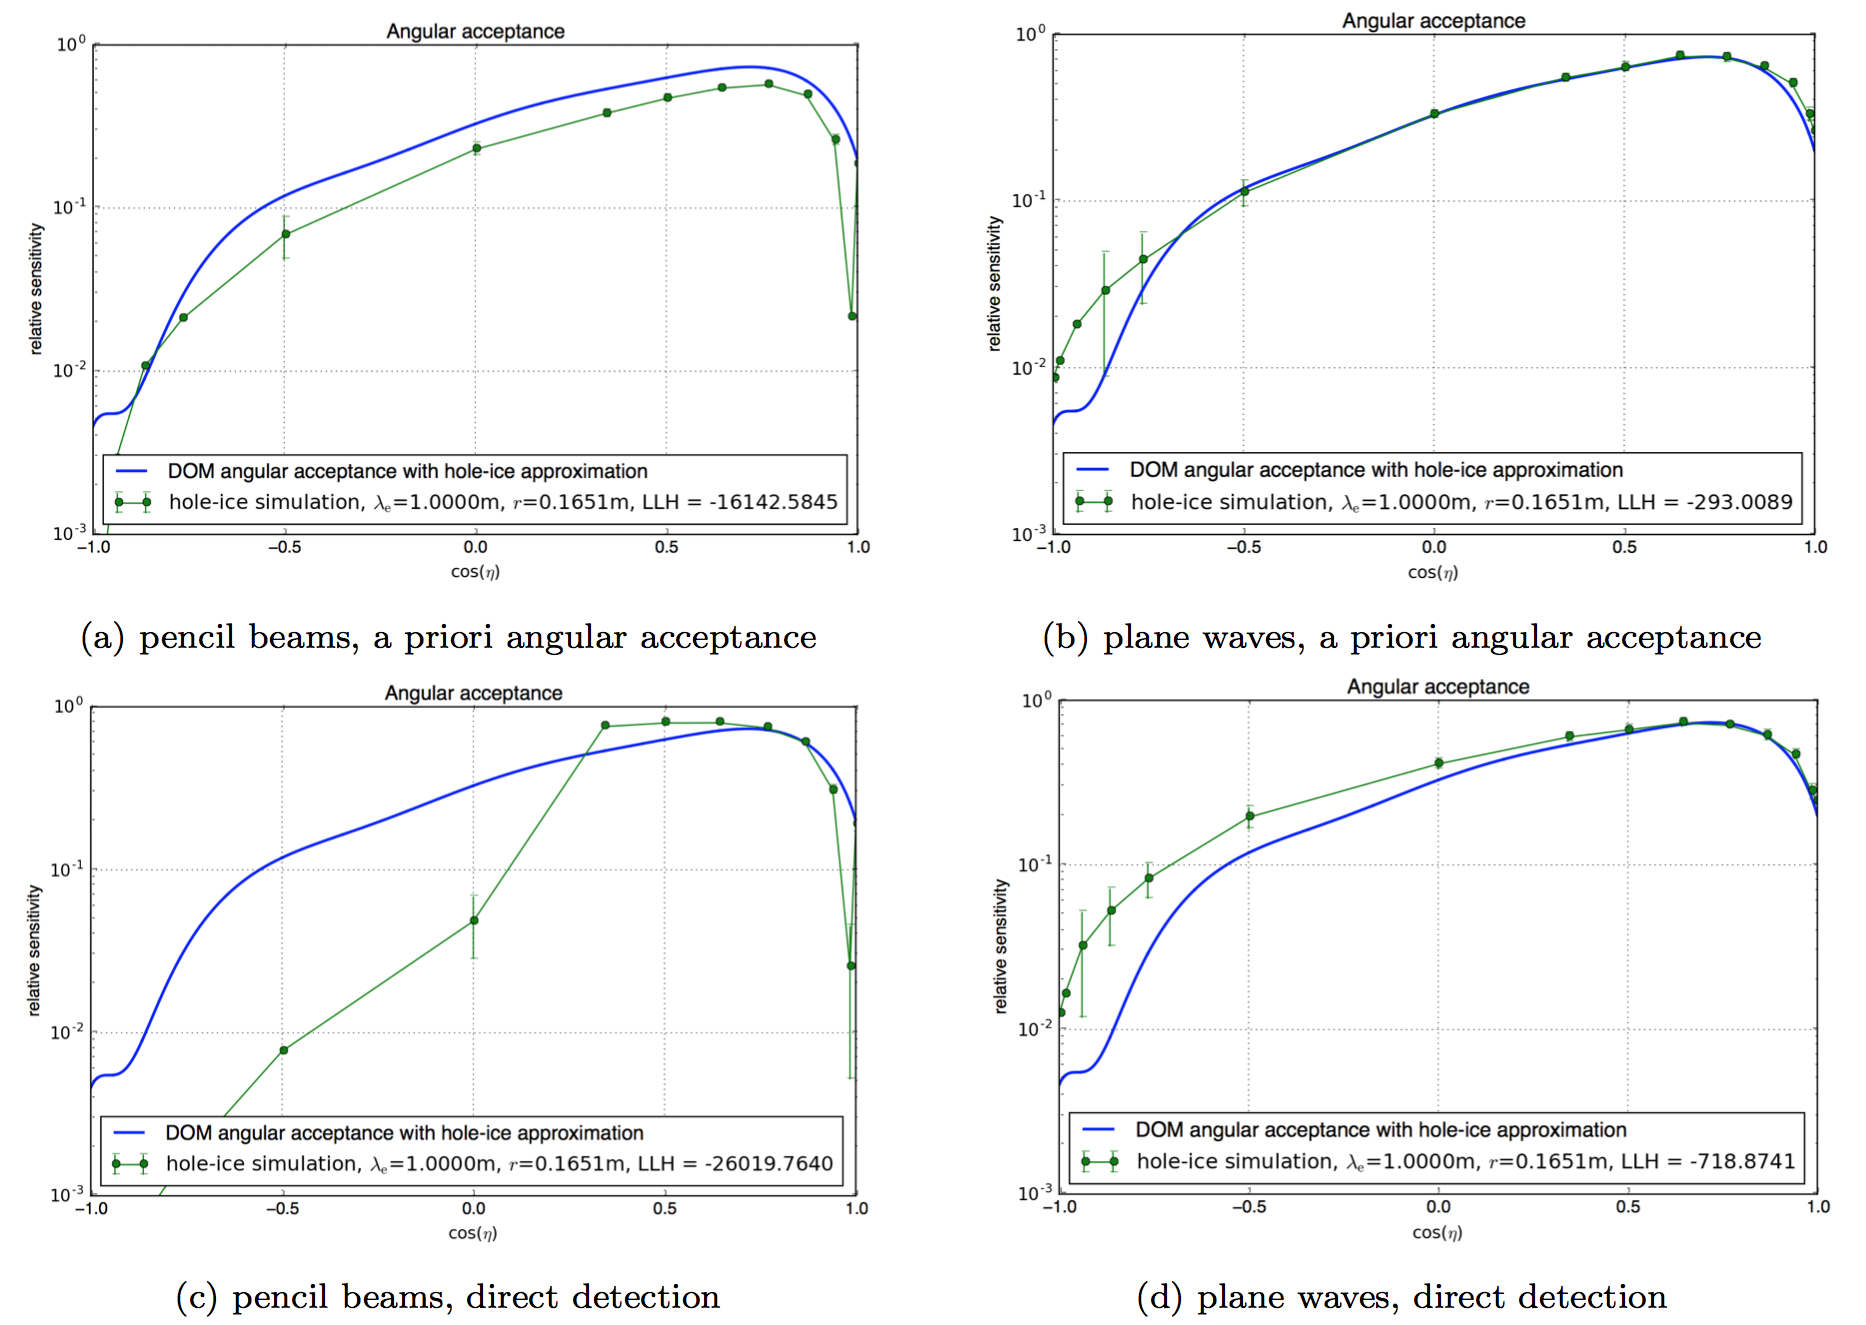
\includegraphics[width=0.7\textwidth]{img/angular-acceptance-methods-with-hole-ice}}
  \end{center}

  \source{\url{https://github.com/fiedl/hole-ice-study/issues/98} and \url{https://github.com/fiedl/hole-ice-study/issues/99}}
\end{frame}


\subsection{Algorithm}
  %!TEX TS-program = ../make.zsh

\begin{frame}{Simplified simulation-step flow chart}
  \begin{center}
    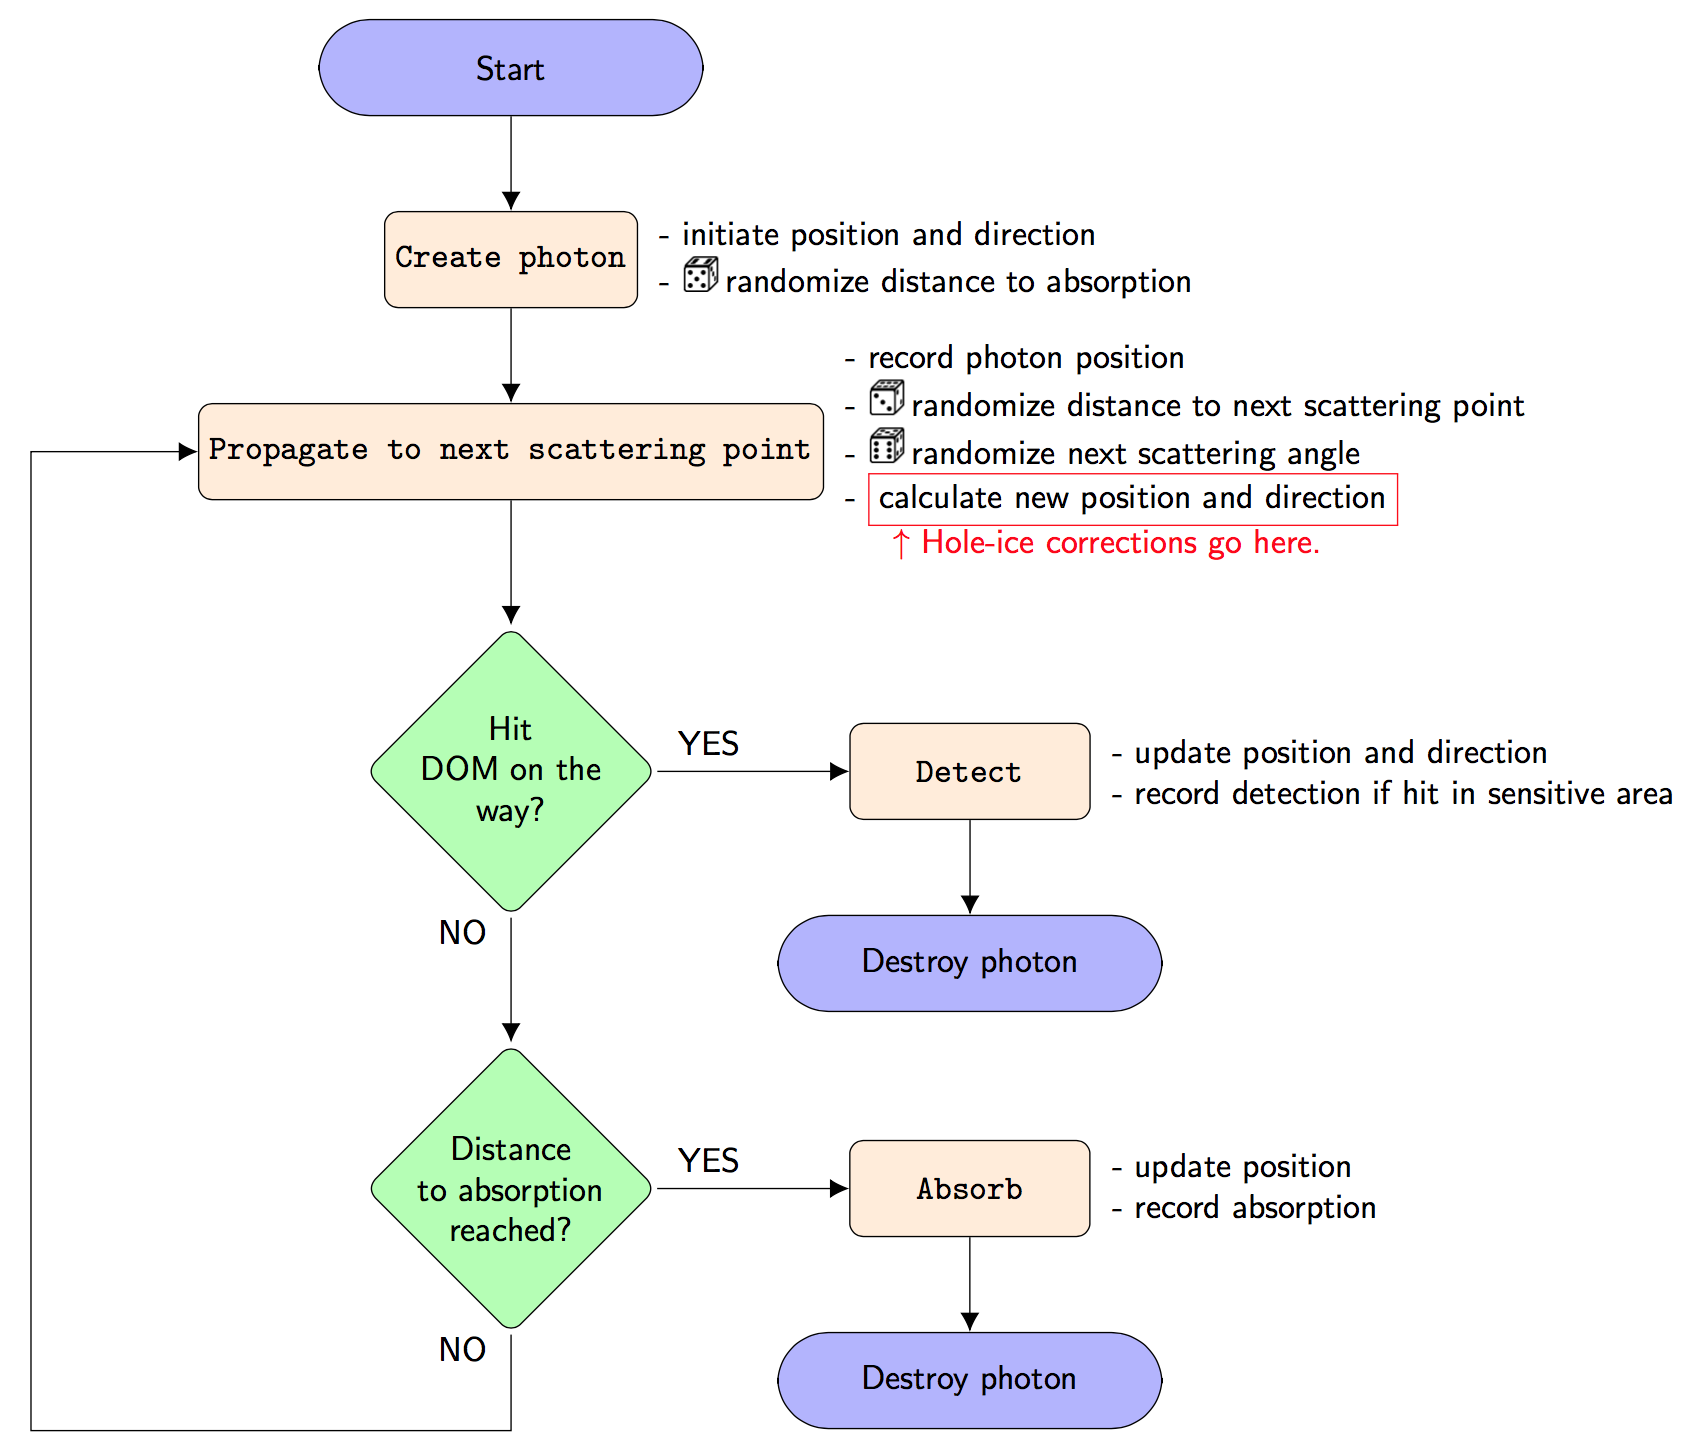
\includegraphics[height=0.8\textheight]{img/simulation-step-flow-chart}
  \end{center}

  \source{\url{https://github.com/fiedl/hole-ice-study/issues/75}}
\end{frame}

\subsection{Cross checks}
  %\begin{frame}[fragile]{Instant absorption}

  Visualizing instant absorption with clsim and steamshovel.
  \small{DOM radius: 10\cm, hole ice radius: 30\cm}

  \begin{onlyenv}<1>
    \begin{sideimage}{img/instant-absorption-3d}
      Photon point source, 3d view

      \begin{bash}
        $ICESIM/env-shell.sh
        cd $HOLE_ICE_STUDY/scripts/FiringRange
        ./run.rb \
            --scattering-factor=1.0 --absorption-factor=0.0 \
            --distance=1.0 \
            --number-of-photons=1e3 --angle=90 \
            --number-of-runs=1 --number-of-parallel-runs=1 \
            --save-photon-paths --cpu
        steamshovel tmp/propagated_photons.i3
      \end{bash}
    \end{sideimage}
  \end{onlyenv}

  \begin{onlyenv}<2>
    \begin{sideimage}{img/instant-absorption-top}
      Plane wave photon source, top view

      \begin{bash}
        $ICESIM/env-shell.sh
        cd $HOLE_ICE_STUDY/scripts/FiringRange
        ./run.rb \
            --scattering-factor=1.0 --absorption-factor=0.0 \
            --distance=1.0 --plane-wave \
            --number-of-photons=1e3 --angle=90 \
            --number-of-runs=1 --number-of-paralle-runs=1 \
            --cpu --save-photon-paths
        steamshovel tmp/propagated_photons.i3
      \end{bash}
    \end{sideimage}
  \end{onlyenv}

  \source{\url{https://github.com/fiedl/hole-ice-study/issues/22}}
\end{frame}

  %!TEX TS-program = ../make.zsh

\begin{frame}[fragile]{Instant absorption with nested cylinders}

  The inner cylinder is configured for small scattering length, the outer cylinder for instant absorption. \\

  \begin{columns}
    \begin{column}{0.5\textwidth}

      \image{containment-example}

      With outer cylinder configured for instant absorption

    \end{column}
    \begin{column}{0.5\textwidth}

      \only<1>{
        \image{containment-example-2d}

        Top view
      }
      \only<2>{
        \image{containment-example-without-outer-cylinder}

        Without the outer cylinder
      }

    \end{column}
  \end{columns}

  % Visualizing instant absorption with clsim and steamshovel.
  % \small{DOM radius: 10\cm, hole ice radius: 30\cm}
  %
  % \begin{onlyenv}<1>
  %   \begin{sideimage}{img/instant-absorption-3d}
  %     Photon point source, 3d view
  %
  %     \begin{bash}
  %       $ICESIM/env-shell.sh
  %       cd $HOLE_ICE_STUDY/scripts/FiringRange
  %       ./run.rb \
  %           --scattering-factor=1.0 --absorption-factor=0.0 \
  %           --distance=1.0 \
  %           --number-of-photons=1e3 --angle=90 \
  %           --number-of-runs=1 --number-of-parallel-runs=1 \
  %           --save-photon-paths --cpu
  %       steamshovel tmp/propagated_photons.i3
  %     \end{bash}
  %   \end{sideimage}
  % \end{onlyenv}
  %
  % \begin{onlyenv}<2>
  %   \begin{sideimage}{img/instant-absorption-top}
  %     Plane wave photon source, top view
  %
  %     \begin{bash}
  %       $ICESIM/env-shell.sh
  %       cd $HOLE_ICE_STUDY/scripts/FiringRange
  %       ./run.rb \
  %           --scattering-factor=1.0 --absorption-factor=0.0 \
  %           --distance=1.0 --plane-wave \
  %           --number-of-photons=1e3 --angle=90 \
  %           --number-of-runs=1 --number-of-paralle-runs=1 \
  %           --cpu --save-photon-paths
  %       steamshovel tmp/propagated_photons.i3
  %     \end{bash}
  %   \end{sideimage}
  % \end{onlyenv}

  \source{\url{https://github.com/fiedl/hole-ice-study/issues/47}}
\end{frame}

  %!TEX TS-program = ../make.zsh

\begin{frame}[fragile]{Scattering example}

  \begin{columns}
    \begin{column}{0.5\textwidth}

      \image{abs-len-about-5cm-sca-0-001-steamshovel}

    \end{column}

    \begin{column}{0.5\textwidth}

      \begin{itemize}
        \item Hole-ice absorption length: about 5\cm
        \item Hole-ice scattering length factor: 0.001
      \end{itemize}

      \begin{smallbash}
        $ICESIM/env-shell.sh
        cd $HOLE_ICE_STUDY/scripts/FiringRange
        ./run.rb --scattering-factor=0.001 --absorption-factor=0.00033 --distance=1.0 --number-of-photons=100 --number-of-runs=1 --number-of-parallel-runs=1 --save-photon-paths --cpu --plane-wave
        steamshovel tmp/propagated_photons.i3
      \end{smallbash}

    \end{column}

  \end{columns}
\end{frame}
  %!TEX TS-program = ../make.zsh

\begin{frame}[fragile]{Cross checks: Arrival-time distributions}
  \image{cross-check-91-arrival-time}
  \source{\url{https://github.com/fiedl/hole-ice-study/issues/91}. Image based on \url{https://wiki.icecube.wisc.edu/index.php/File:Distances.i86.jpg}.}
\end{frame}

\begin{frame}[fragile]{Cross checks: Path-length distributions}
  \begin{column}{0.5\textwidth}
    \image{cross-check-66-steamshovel}
  \end{column}
  \begin{column}{0.5\textwidth}
    \image{cross-check-66-path-length-histogram}
  \end{column}
  \source{\url{https://github.com/fiedl/hole-ice-study/issues/66}}
\end{frame}

\begin{frame}[fragile]{Cross checks: Distance to next scattering point vs. dst. from hole-ice center}
  \image{cross-check-71-sca-distance}
  \source{\url{https://github.com/fiedl/hole-ice-study/issues/71}}
\end{frame}


\subsection{Examples}
  \include{text/short_scattering_example}
  %!TEX TS-program = ../make.zsh

\begin{frame}[fragile]{Separate hole-ice cylinder positions}

  \begin{columns}
    \begin{column}{0.5\textwidth}

      \image{cylinder-shift-steamshovel}

    \end{column}
    \begin{column}{0.5\textwidth}

      \begin{itemize}
        \item Each string can have its own hole-ice cylinder configuration
          \begin{itemize}
            \item cylinder position
            \item cylinder radius
            \item DOM positions --- DOMs may not be perfectly centred relative to the hole ice
          \end{itemize}

        \item Currently configurable in Geometry frame. \\

          \textbf{Q: Is there a better place to configure this?}
          \note{Cylinder configuration needs to be accessible by the steamshovel artist.}

        \item Still work to be done:
          \begin{itemize}
            \item Ice properties need to be configurable for each cylinder:
                \tiny \url{https://github.com/fiedl/hole-ice-study/issues/9} \small
          \end{itemize}
      \end{itemize}


    \end{column}
  \end{columns}

\end{frame}



  %!TEX TS-program = ../make.zsh

\begin{frame}[fragile]{Asymmetry example}

  \begin{columns}
    \begin{column}{0.5\textwidth}

      \only<1>{\image{asymmetry-example-steamshovel}}
      \only<2>{\image{asymmetry-example-angular-acceptance-with-comment}}

    \end{column}
    \begin{column}{0.5\textwidth}

      \only<1>{For angle $\eta = \pi / 2$,}
      \only<2>{For each angle $\eta \in [0;2\,\pi[$,}
      shoot photons from planes onto the DOM and count hits.

      \small{Hole-ice radius: 30\cm}

      \begin{equation*}\begin{align}
        \lambda_\text{sca,hole-ice} &= \frac{1}{10}\, & \lambda_\text{sca,bulk} \\
        \lambda_\text{abs,hole-ice} &= & \lambda_\text{sca,bulk}
      \end{align}\end{equation*}

      The \textbf{hole-ice is shifted in x-direction against the DOM} position by 20\cm.

      \begin{onlyenv}<1>
        \begin{bash}
          $ICESIM/env-shell.sh
          cd $HOLE_ICE_STUDY/scripts/AngularAcceptance
          ./run.rb --scattering-factor=0.1 --absorption-factor=1.0 --distance=1.0 --plane-wave --number-of-photons=1e2 --cylinder-shift=0.2 --save-photon-paths --cpu
          steamshovel tmp/propagated_photons.i3
        \end{bash}
      \end{onlyenv}

      \begin{onlyenv}<2>
        \begin{smallbash}
          $ICESIM/env-shell.sh
          cd $HOLE_ICE_STUDY/scripts/AngularAcceptance
          ./run.rb --scattering-factor=0.1 --absorption-factor=1.0 --distance=1.0 --plane-wave --number-of-photons=1e5 --angles=0,10,20,30,40,50,60,70,90,120,140,150,160,170,190,200,210,220, 240,260,270,290,300,310,320,330,340,350 --number-of-runs=2 --number-of-parallel-runs=2 --cylinder-shift=0.2
          open results/current/plot_with_reference.png
        \end{smallbash}
      \end{onlyenv}

    \end{column}
  \end{columns}

  \source{\url{https://github.com/fiedl/hole-ice-study#asymmetry-example}, \url{https://github.com/fiedl/hole-ice-study/issues/8}}

\end{frame}

\note[itemize]{
  \item In data points, one sees upper curve and lower curve.
  \item Because of the asymmetry, on one way, the distance through the hole ice is smaller, on the other way, larger.
}
  %!TEX TS-program = ../make.zsh

\begin{frame}[fragile]{Cable shadows}

  \begin{columns}
    \begin{column}{0.5\textwidth}

      \image{cable-shadow-steamshovel}

    \end{column}
    \begin{column}{0.5\textwidth}

      \begin{itemize}
        \item Cables can be modelled as separate cylinders
          \begin{itemize}
            \item for each DOM separate position
            \item 1\,m height
            \item configured for instant absorption
          \end{itemize}
        \item This image:
          \begin{itemize}
            \item DOM radius: 16.5\cm
            \item bubble-column radius: 8.0\cm
            \item cable radius: 2.0\cm
          \end{itemize}
        \item Still work to be done:
          \begin{itemize}
            \item z-range needs to be implemented in hole-ice code:
                \tiny \url{https://github.com/fiedl/hole-ice-study/issues/34} \small
          \end{itemize}
      \end{itemize}


    \end{column}
  \end{columns}

  \source{\url{https://github.com/fiedl/hole-ice-study/issues/35}}
\end{frame}
  %!TEX TS-program = ../make.zsh

\begin{frame}[fragile]{Direct cable simulation: Angular acceptance}

  \begin{column}{0.3\textwidth}
    \image{dom-deployment-15-IMG_0080-652058109-3}
  \end{column}
  \begin{column}{0.3\textwidth}
    \image{DOMCloseUp-cropped-mirrored}
  \end{column}
  \begin{column}{0.3\textwidth}
    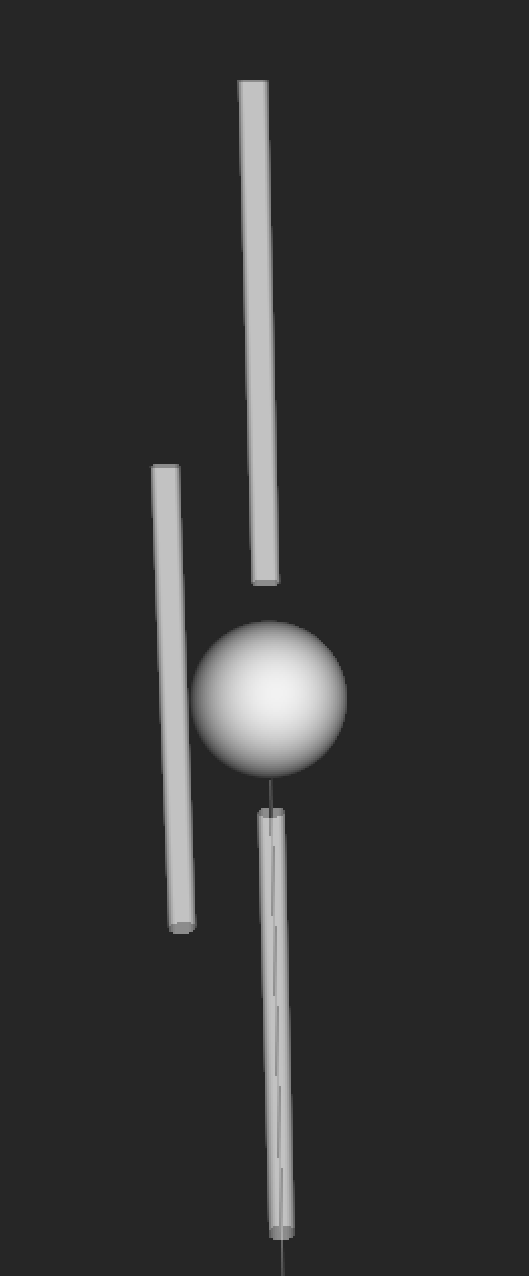
\includegraphics[height=0.8\textheight]{img/cable-only-vs-h2-steamshovel}
  \end{column}

  \source{\url{https://github.com/fiedl/hole-ice-study/issues/101}. \her{Images}: \url{https://icecube.wisc.edu/gallery/view/153}, \url{https://gallery.icecube.wisc.edu/internal/v/GraphicRe/graphics/arraygraphics2011/sketchup/DOMCloseUp.jpg.html}}

\end{frame}


\begin{frame}[fragile]{Direct cable simulation: Angular acceptance}

  \begin{column}{0.6\textwidth}
    \image{cable-only-vs-h2-angular-acceptance}
  \end{column}
  \begin{column}{0.3\textwidth}
    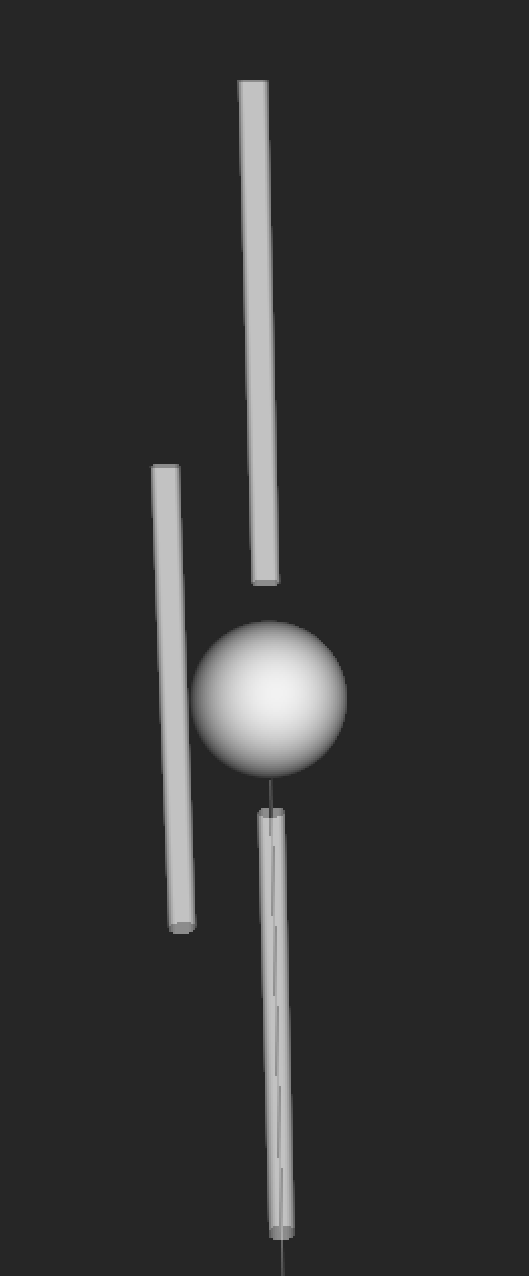
\includegraphics[height=0.8\textheight]{img/cable-only-vs-h2-steamshovel}
  \end{column}

  \source{\url{https://github.com/fiedl/hole-ice-study/issues/101}.}

\end{frame}

  %!TEX TS-program = ../make.zsh

\begin{frame}[fragile]{Nested hole-ice cylinders}

  \begin{columns}
    \begin{column}{0.5\textwidth}

      \image{nested-cylinders-steamshovel-annotated}

    \end{column}
    \begin{column}{0.5\textwidth}

      \begin{itemize}
        \item Hole-ice cylinders can be nested
          \begin{itemize}
            \item for each string separate positions
            \item for each string and each column separate radii
          \end{itemize}
        \item This image:
          \begin{itemize}
            \item DOM radius: 16.5\cm
            \item bubble-column radius: 8.0\cm
            \item outer-column radius: 30.0\cm
          \end{itemize}
        \item Still work to be done:
          \begin{itemize}
            \item Ice properties need to be configurable for each cylinder:
                \tiny \url{https://github.com/fiedl/hole-ice-study/issues/9} \small
          \end{itemize}
      \end{itemize}


    \end{column}
  \end{columns}

  \source{\url{https://github.com/fiedl/hole-ice-study/issues/7}}
\end{frame}

  %!TEX TS-program = ../make.zsh

\begin{frame}[fragile]{Realistic simulation scenario} % Nested shifted cylinders and cable}

  \begin{columns}
    \begin{column}{0.6\textwidth}

      \image{cable-inside-shifted-bc-steamshovel}

    \end{column}
    \begin{column}{0.4\textwidth}

      \begin{itemize}
        \item DOM: radius 16.5\cm, shifted by 12.0\cm against the center of the bore hole
        \item bubble column: radius 8.0\cm
        \item drill-hole column: radius 30.0\cm
        \item cable: radius 3.0\cm, placed next to the DOM, partially within the bubble column
      \end{itemize}

      \vspace{1cm}
      \vtiny{See also: \url{https://github.com/fiedl/hole-ice-study/issues/110}}
    \end{column}
  \end{columns}

\end{frame}

  %!TEX TS-program = ../make.zsh

\begin{frame}{Flasher-simulation example}

  Calibration: Find out the properties of the hole ice by comparing simulations with differnt properties to data of IceCube's LED-flasher-calibration system.\\

  \centering
  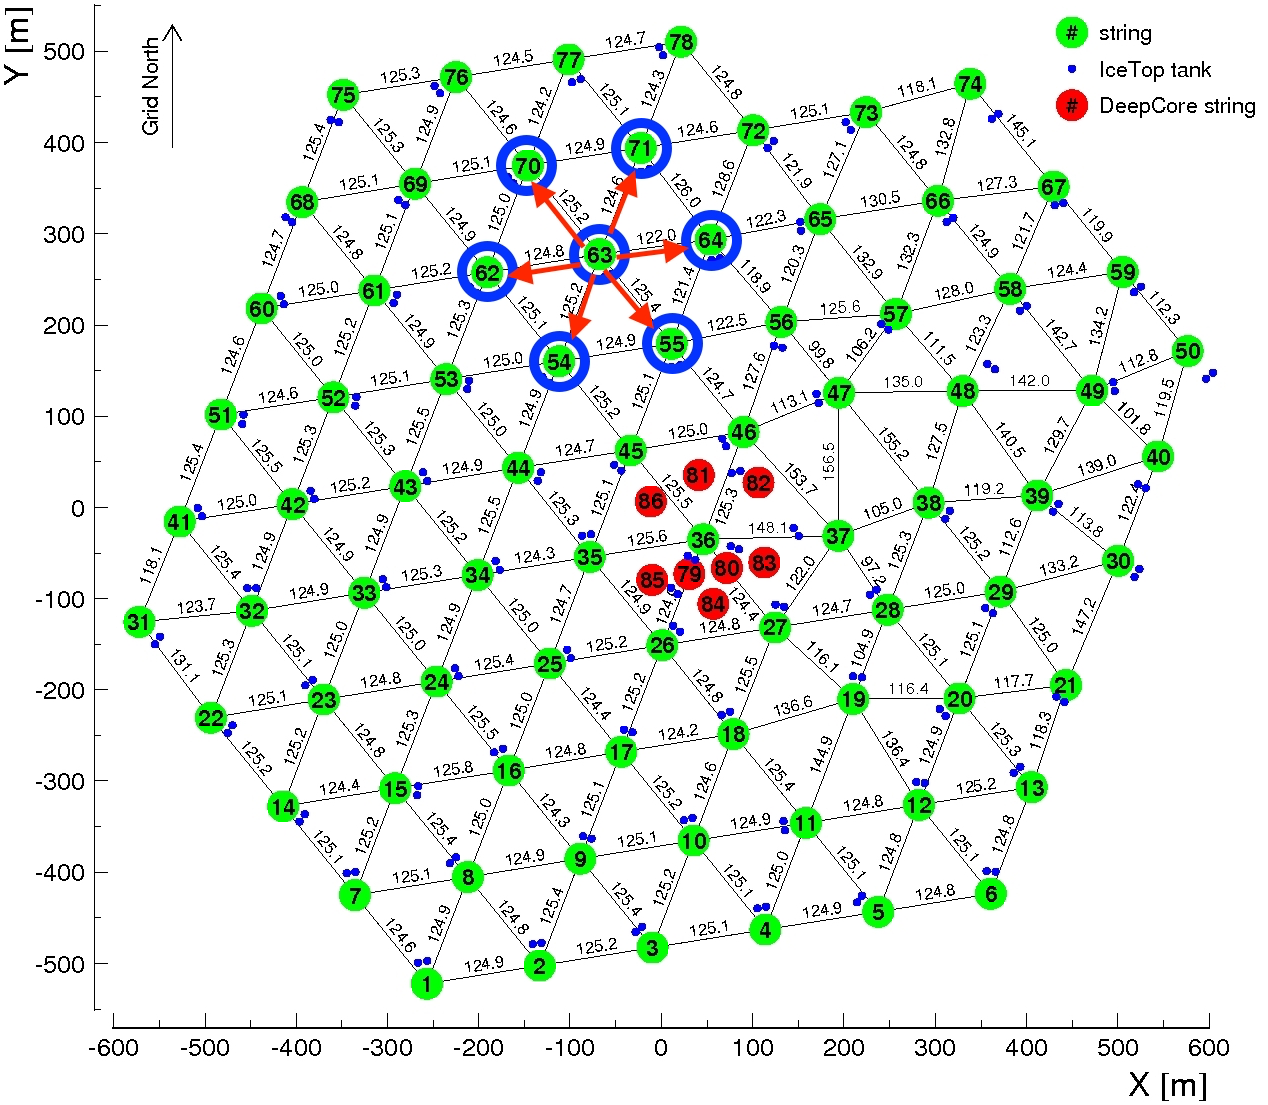
\includegraphics[height=0.35\textheight]{img/flasher-scenario}\hspace{1.2cm}
  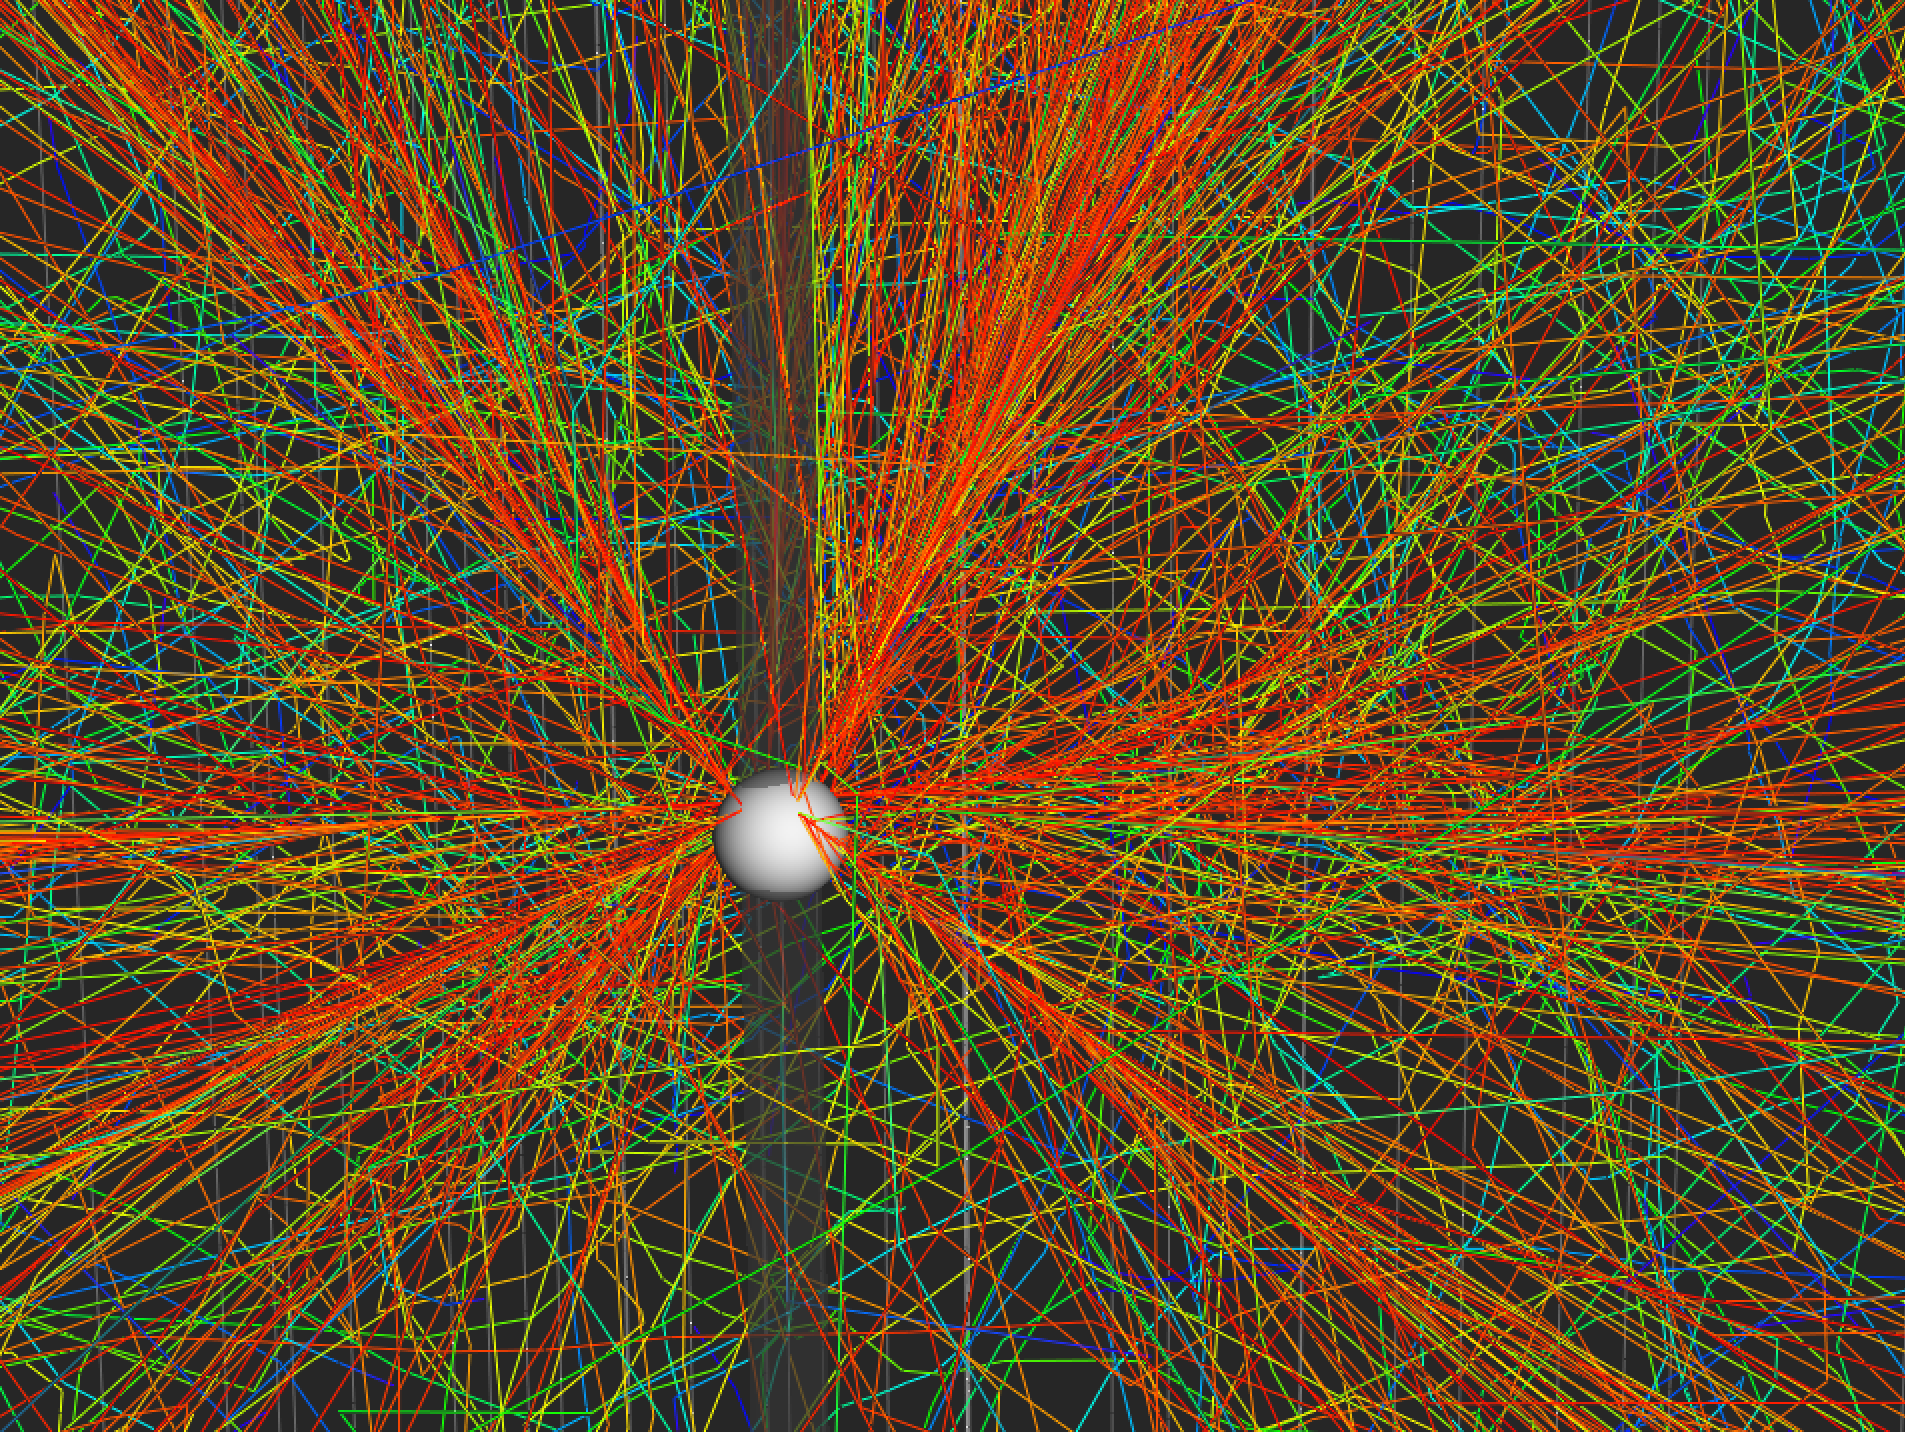
\includegraphics[height=0.35\textheight]{img/flasher-steamshovel-sending}

  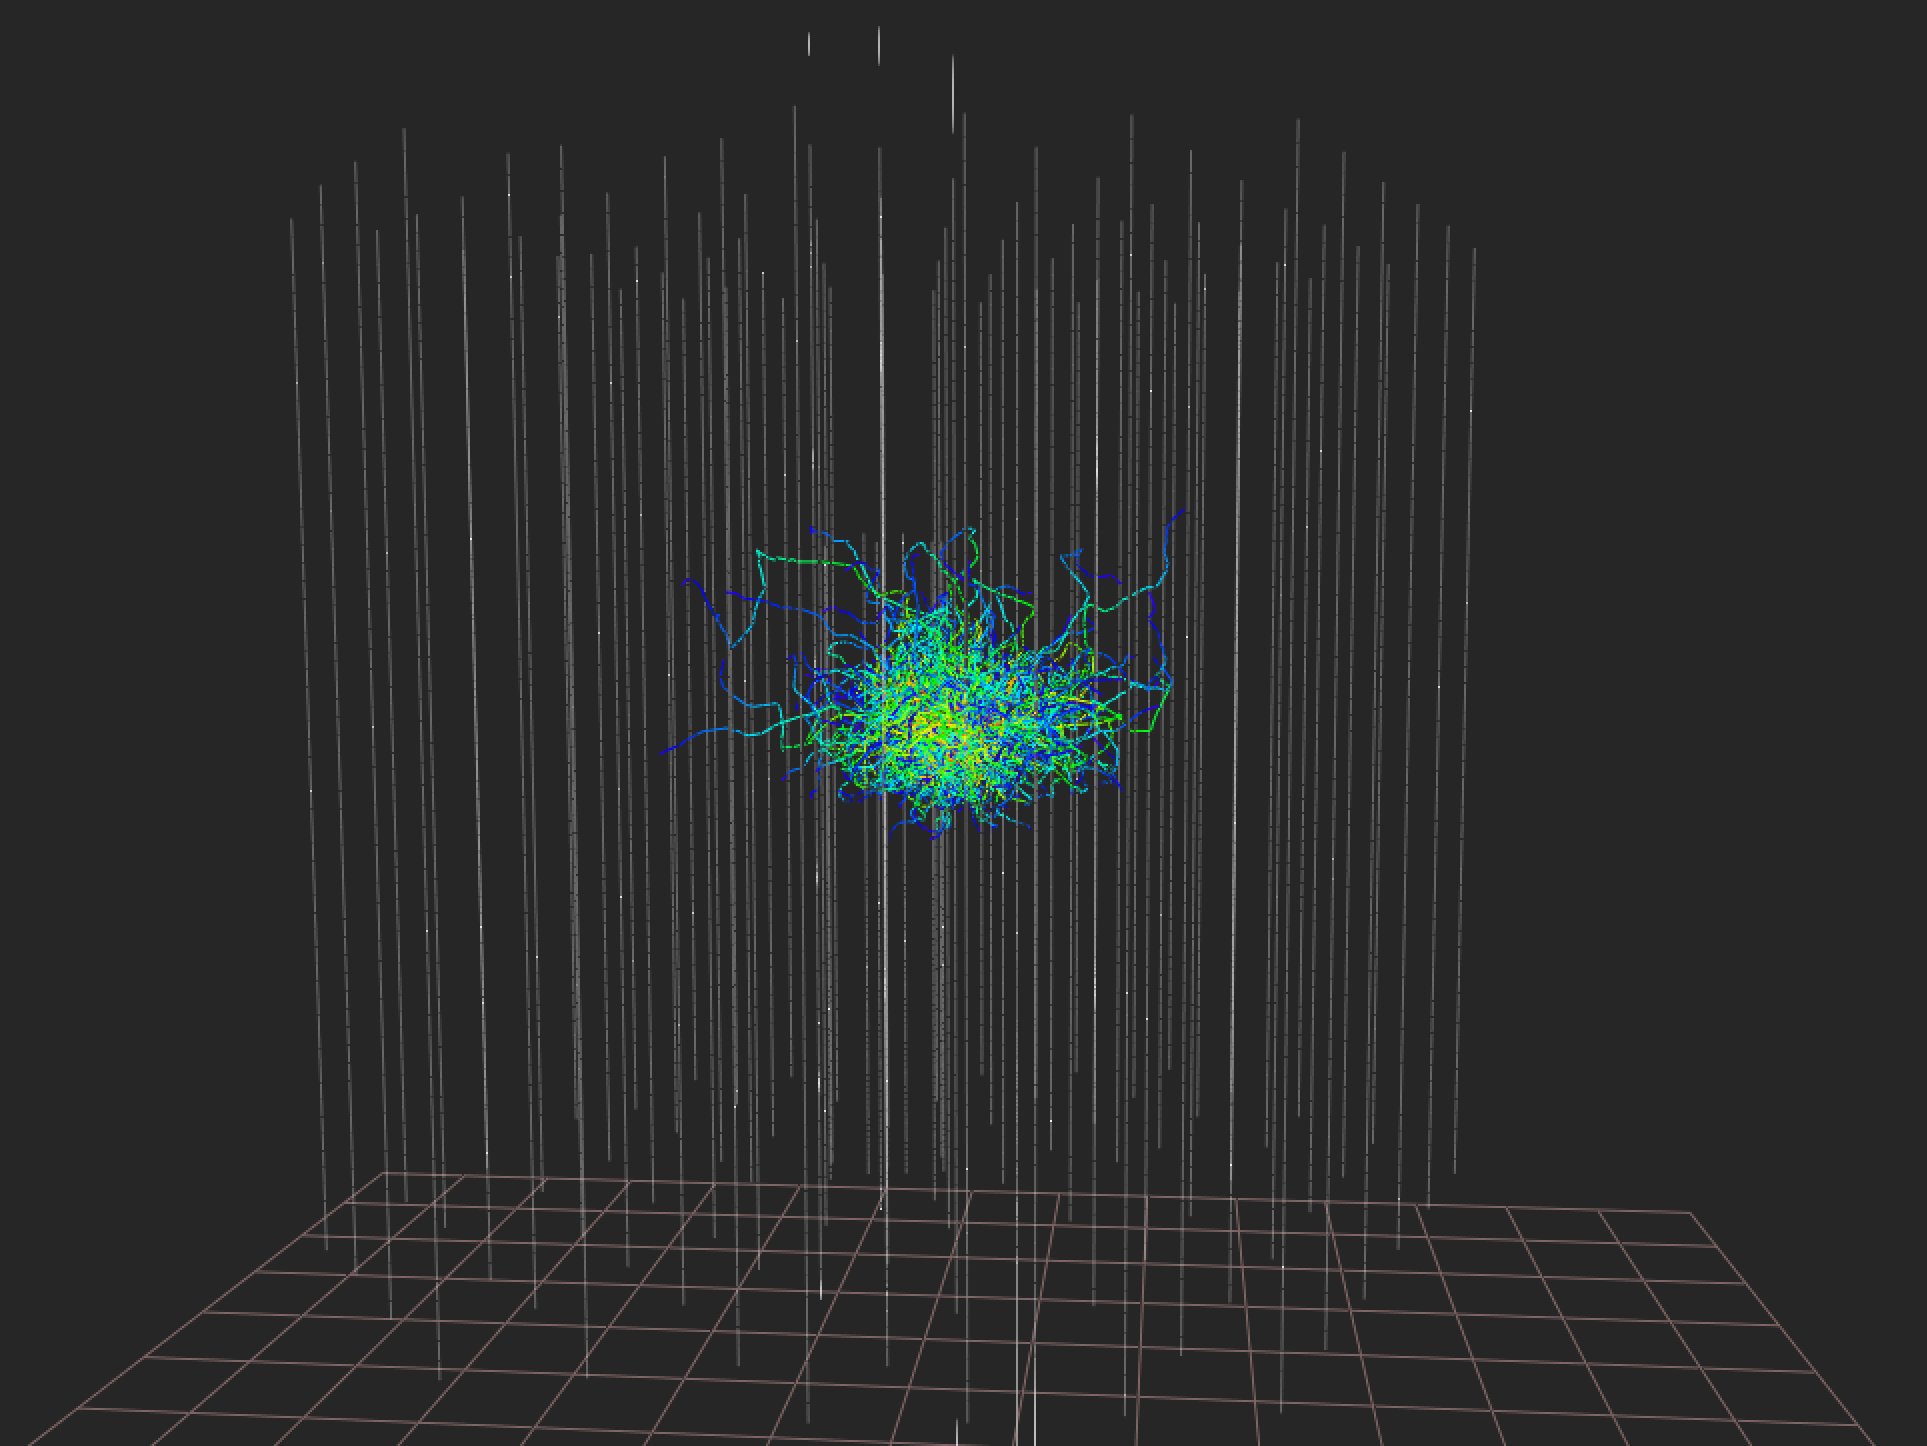
\includegraphics[height=0.35\textheight]{img/flasher-steamshovel-total}\hspace{3mm}
  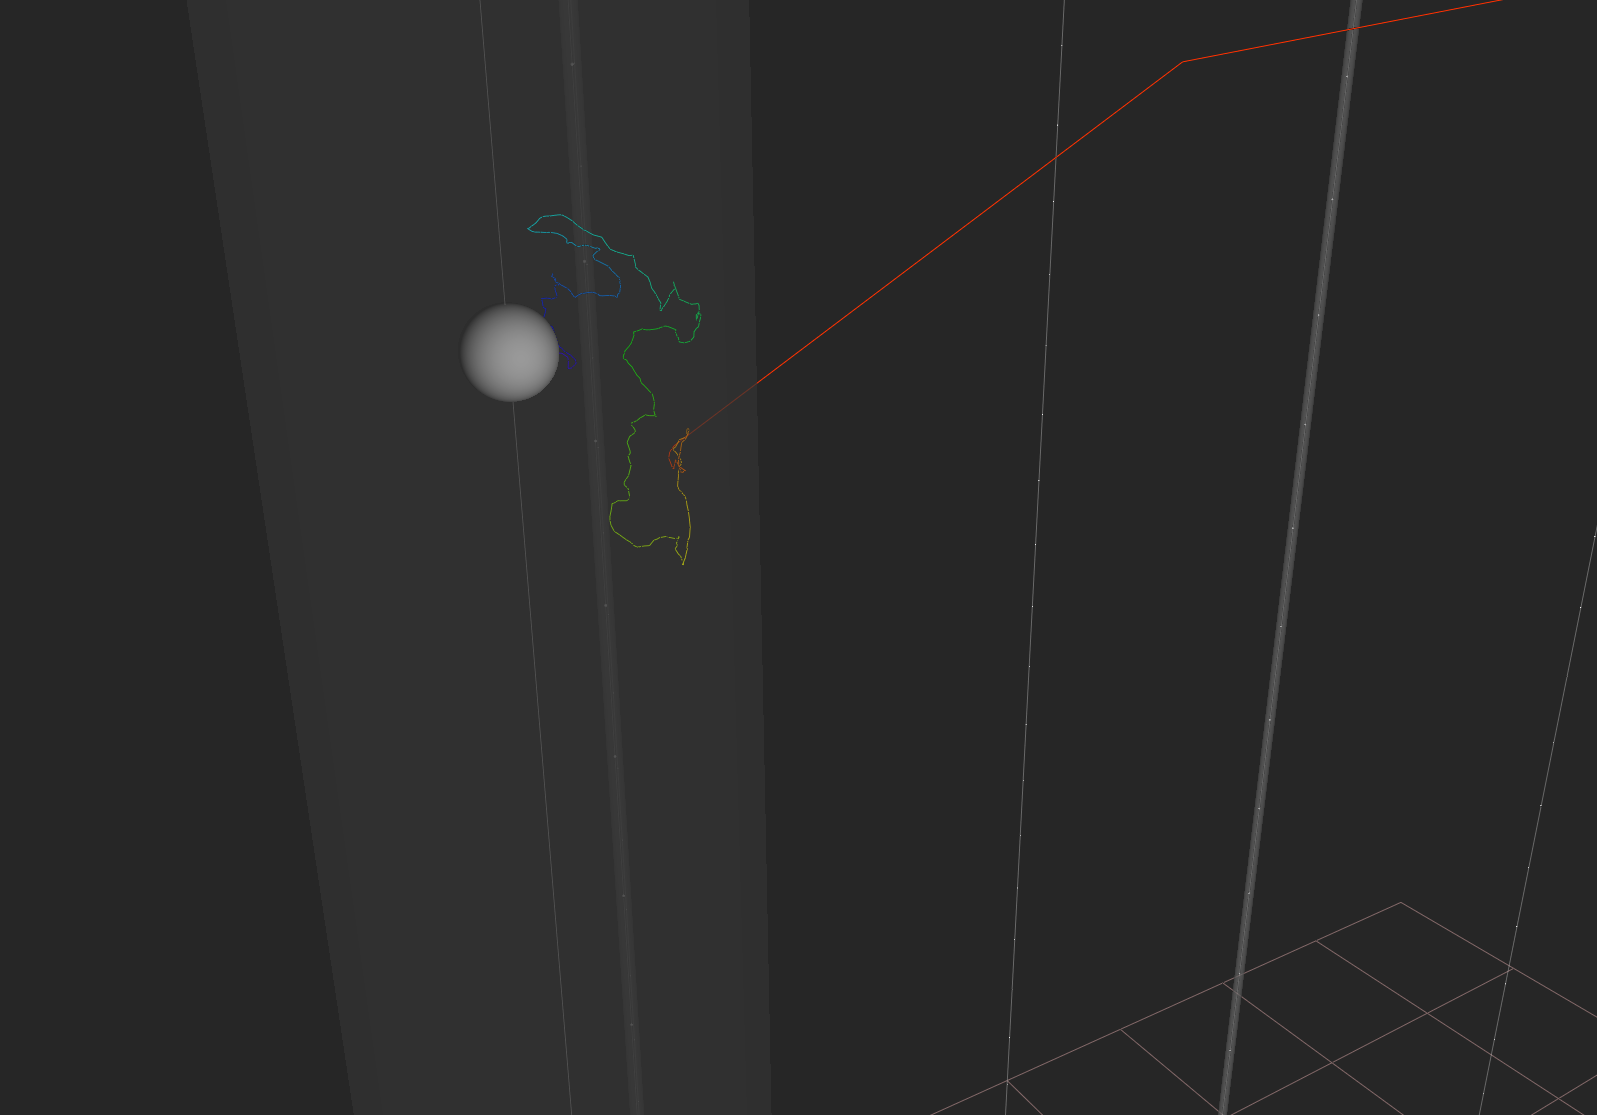
\includegraphics[height=0.35\textheight]{img/flasher-steamshovel-single-received-photon}

  \tiny{See \url{https://github.com/fiedl/hole-ice-study/issues/107}}

\end{frame}

  %!TEX TS-program = ../make.zsh

\begin{frame}[fragile]{Early results: Example scan for best hole-ice parameters based on calibration data}
  \begin{column}{0.5\textwidth}
    \image{flasher-scenario-light}
  \end{column}
  \begin{column}{0.5\textwidth}
    \image{flasher-contours-59}
  \end{column}

  \source{\url{https://github.com/fiedl/hole-ice-study/issues/59}. Image based on \url{https://wiki.icecube.wisc.edu/index.php/File:Distances.i86.jpg}.}
\end{frame}

% \begin{frame}[fragile]{Flasher parameter scan vs. SpiceHD scan}
%   \begin{column}{0.5\textwidth}
%     SpiceHD with ppc: \medskip
%
%     \image{flasher-contours-martin}
%
%     DOM positions are fit parameters.
%   \end{column}
%   \begin{column}{0.5\textwidth}
%     clsim with direct hole ice: \medskip
%
%     \image{flasher-same-color-axis-as-spicehd}
%
%     All DOMs perfectly centered within hole ice.
%   \end{column}
%
%   \bigskip
%   Mind systematics: DOM displacement does account for the observed scattering-length factor $\frac{1}{3}$ for the hole-ice radius of 1.8 dom radii (right-hand side of the plot).
%
%   \source{\url{https://github.com/fiedl/hole-ice-study/issues/106}. }
% \end{frame}
  %!TEX TS-program = ../make.zsh

\begin{frame}[fragile]{Direct cable simulation: Flasher}
  \begin{column}{0.5\textwidth}
    \only<1-2>{\image{flasher-scenario}}
    \only<3-4>{\image{flasher-scenario-with-cable}}
  \end{column}
  \begin{column}{0.5\textwidth}
    \only<2-3>{\image{flasher-data-2012}}
    \only<4>{\image{flasher-simulation-with-cable-vs-data}}
  \end{column}

  \source{\url{https://github.com/fiedl/hole-ice-study/issues/97}. Image based on \url{https://wiki.icecube.wisc.edu/index.php/File:Distances.i86.jpg}.}
\end{frame}

%
% %\subsection{State of the hole-ice simulation}
% %  %!TEX TS-program = ../make.zsh

\newcommand\done{\checkmark\xspace}
\newcommand\inprogress{$\Rightarrow$\xspace}
\newcommand\tobedone{$\square$\xspace}

\section{Overview}
\subsection{Goal and Context}
\begin{frame}[fragile]{Overview: Goal and Context}
  \begin{columns}
    \begin{column}{0.65\textwidth}
      \begin{description}
        \item[Origin] \her{Diploma thesis} (2018-09) implementing direct photon propagation through hole ice in clsim in order to study hole-ice effects and improve understanding of low-energy systematics. \small \url{https://github.com/fiedl/hole-ice-study} \normalsize

        \item[Goal] \her{Bring} the new simulation \her{into} the icecube-simulation \her{framework} such that other icecubers can use it.

        \item[Context] \her{Service work} for the icecube collaboration in the beginning of my time as PhD student with icecube at ECAP/Erlangen.

        \item[Time frame] about 6 months
      \end{description}

      \source{\underline{Top}: Rongen: The 2018 Sweden Camera run — light at the end of the ice, 2018. \underline{Bottom}: \url{https://github.com/fiedl/hole-ice-study/issues/107}}
    \end{column}
    \begin{column}{0.35\textwidth}
      \image{camera2018-01}

      % https://github.com/fiedl/hole-ice-study/issues/107
      \image{flasher-steamshovel-single-received-photon}
    \end{column}
  \end{columns}
\end{frame}

\subsection{Work to be done}
\begin{frame}{Overview: Work to be done}

  %\begin{itemize}
  %
  %
  %  \item[\done] Compile current icecube-simulation release V06-01-01 with Python 3 locally
  %  \item[\done] Make hole-ice code work with current icecube-simulation release V06-01-01
  %  \item[\inprogress] Provide example scripts for Python 3 (rather than Ruby)
  %  \item[\inprogress] Synchronize svn and git repositories of clsim
  %  \item[\tobedone] Re-implement ice tilt and ice anisotropy
  %  \item[\tobedone] Implement direct-detection switch
  %  \item[\tobedone] Merge hole-ice code into clsim trunk
  %\end{itemize}

  \setbeamertemplate{subsection in toc}{\hspace*{1em} \inserttocsubsection \vspace{2ex} \par}
  \tableofcontents[sectionstyle=hide,subsectionstyle=show,sections=2-]

  \bigskip \bigskip \small
  \done = done \ \ \ \inprogress = work in progress \ \ \ \tobedone\ = still to do
\end{frame}

\section{State of the individual steps}
\subsection{\done Compile IceSim V06-01-01 with Python 3}
\begin{frame}{\done Compile IceSim V06-01-01 with Python 3}
  \begin{itemize}
    \item In Stockholm (2018-09), the icecube software group requested the hole-ice example scripts to be provided in Python 3 (rather than Python 2 or Ruby) in order to push the migration to Python 3 forward.
    \item The current icecube documentation on how to install the framework on macOS still assumes Python 2: \url{http://software.icecube.wisc.edu/documentation/projects/cmake/supported_platforms/osx.html}
    \item[\done] Using Vagrant, a virtual-machine wrapper, I've documented a clean, reproducible way to install icecube-simulation V06-01-01 on macOS Sierra, which I use locally.
    \item[\done] Found a couple of issues and provided patches.
    \item[\tobedone] Still need to talk to the software group. Maybe they want to link or import the install  documentation.
    \item[\tobedone] I would love to run this on Travis-CI. But this would expose the build logs (no credentials) to the public. Need to check with software group whether this would be ok.
  \end{itemize}

  \bigskip \her{Documented at: \url{https://github.com/fiedl/hole-ice-install}} \bigskip
\end{frame}

\subsection{\inprogress Port hole-ice code to clsim of icecube-simulation V06-01-01}
\begin{frame}{\inprogress Port hole-ice code to clsim of icecube-simulation V06-01-01}
  \begin{itemize}
    \item The original study was based on the icecube-simulation framework V05-00-07 from 2016.
    \item From the V05-00-07 (2016) to V06-01-01 (2019), there are 93 commits in clsim. A lot has changed.
    \item There are two separate repositories for original clsim, in addition to the hole-ice fork, which need to be kept in sync. For my work, I have forked Claudio's repository on github. But now, Claudio's github repository is behind the current work in the SVN repository. \\
      \url{http://code.icecube.wisc.edu/svn/projects/clsim} \\
      \url{https://github.com/claudiok/clsim} \\
      \url{https://github.com/fiedl/clsim}
    \item[\done] Find common interface to sync the repositories: \texttt{git-svn}
    \item[\inprogress] Coordinating with the clsim maintainer, Claudio Kopper: The repositories need to be synced before the code can be ported to avoid conflicts later.
    \item[\tobedone] Rebase the hole-ice changes onto the V06-01-01 release
    \item[\tobedone] Make sure everything is still running
    \item[\tobedone] Make sure there are no conflicts with other attempt on cable shadows
  \end{itemize}
\end{frame}

\subsection{\tobedone Provide example scripts for Python 3}
\begin{frame}[fragile]{\tobedone Provide example scripts for Python 3}
  \begin{columns}
    \begin{column}{0.5\textwidth}
      \begin{itemize}
        \item The example scripts of the original hole-ice study are written in Ruby: \url{https://github.com/fiedl/hole-ice-study}
        \item Icecubers prefer Python instead.
        \item[\inprogress] Together with the calibration group and the POCAM group in Munich, I'm working on a series of hole-ice simulations to study proposed geometries for the icecube upgrade.
        \item[\tobedone] The scripts will be migrated to Python 3, documented, and provided as example scripts for the collaboration.
      \end{itemize}
    \end{column}
    \begin{column}{0.5\textwidth}
      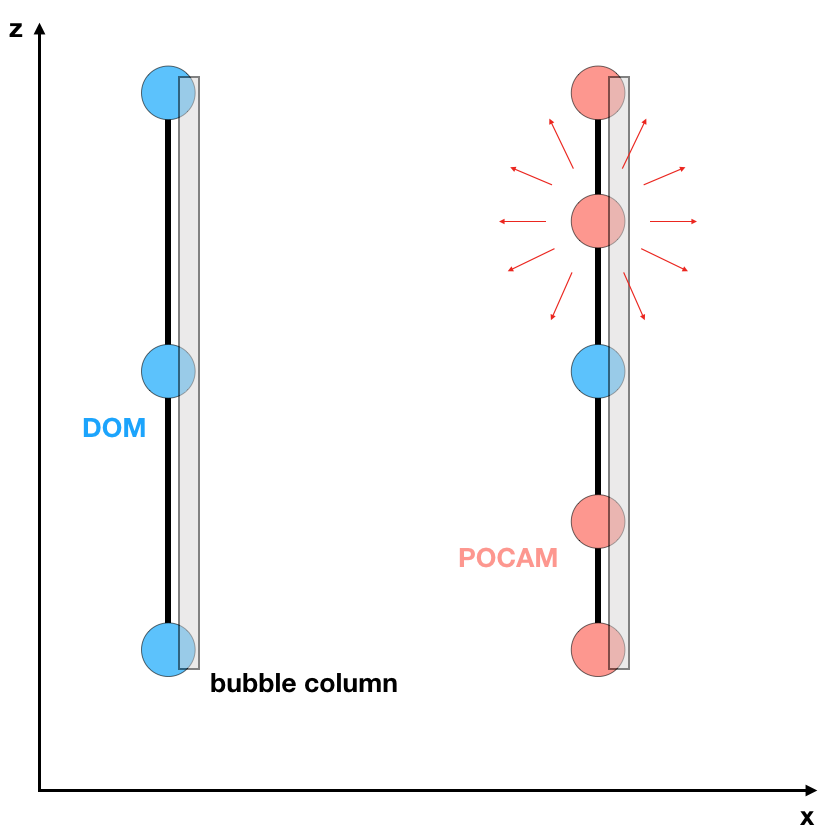
\includegraphics[width=0.8\textwidth]{img/pocamscenario-right}
    \end{column}
  \end{columns}

  \bigskip \her{Example scripts will be at: \url{https://github.com/fiedl/hole-ice-scripts}} \bigskip

  \source{\url{https://github.com/fiedl/hole-ice-talk/releases/tag/v1.5}}
\end{frame}

\subsection{\tobedone Implement missing features}
\begin{frame}{\tobedone Implement missing features}
  \begin{description}
    \item[Ice tilt] Re-implementing ice tilt will be relatively easy after the hole-ice code is ported.
    \item[Direct detection] Direct detection has already been implemented during the original study. But we need a switch to turn it on and off.
    \item[Anisotropy] Instead of re-implementing the old ice-anisotropy model, I'd like to coordinate with Martin Rongen and Dima. Maybe it is possible to implement the new anisotropy model discussed in the previous calibration calls. \url{https://drive.google.com/file/d/1TyqDQgHXSKuHBUC0gLo4xz9RKvxk5dGV/view}
  \end{description}
\end{frame}

\subsection{\tobedone Merge hole-ice code into clsim trunk}
\begin{frame}{\tobedone Merge hole-ice code into clsim trunk}
  \begin{itemize}
    \item When everything works as expected:
    \item[\tobedone] Port hole-ice code to work with svn trunk of the icecube-simulation framework
    \item[\tobedone] Create a feature branch based on the clsim trunk on the svn
    \item[\tobedone] Coordinate with the clsim maintainer, Claudio Kopper, to get it merged into the clsim trunk
  \end{itemize}
\end{frame}

%
% %\subsection{Work to be done}
% %  %!TEX TS-program = ../make.zsh

\begin{frame}{Outlook: What is still missing}
  \begin{itemize}
    \item Re-implement ice tilt and ice anisotropy
    \item Comparison to ppc results
    \item Grid scan to find best match with reference plot
    \item Study performance impact
    \item See also: \url{https://github.com/fiedl/hole-ice-study/issues}
  \end{itemize}
\end{frame}

% %  %!TEX TS-program = ../make.zsh

\newcommand\haken{\checkmark}

\begin{frame}[fragile]{Martin's wish list}
  \begin{tabelle}{L|c|c|c|c}
    \textbf{Feature} & \textbf{Possible} & \textbf{Done} & \textbf{In progress} & \textbf{Will be done by me} \\
    \hline\hline
    Separate hole-ice positions for each string & \haken & \haken & \\ \hline
    Nested cylinders: Bubble column and outer column & \haken & \haken & & \\ \hline
    Cable shadows using cylinder parts & \haken & \haken & & \\ \hline
    Absolute scattering and absorption lengths in hole ice & \haken & \haken & & \\ \hline
    Direct detection & \haken & & \haken & yes \\ \hline
    Bring tilt and anisotropy back & \haken & & & yes \\ \hline
    Gradient of scattering length in bubble column & \haken & & & no \\ \hline
  \end{tabelle}

  \tiny{See also: List of issues on github: \url{https://github.com/fiedl/hole-ice-study/issues}}
\end{frame}
%
% \subsection{DOM oversizing}
%   %!TEX TS-program = ../make.zsh

\begin{frame}[fragile]{DOM oversizing with hole ice?}

  \begin{columns}
    \begin{column}{0.5\textwidth}
      \begin{overlayarea}{\textwidth}{\textheight}
        \vspace*{2cm}
        \only<1>{\image{dom-oversizing-001}}
        \only<2>{\image{dom-oversizing-002}}
        \only<3>{\image{dom-oversizing-003}}
        \only<4>{\image{dom-oversizing-004}}
        \only<5>{\image{dom-oversizing-005}}
      \end{overlayarea}
    \end{column}
    \begin{column}{0.5\textwidth}
      \begin{itemize}
        \item Consider a DOM displaced relative to the bubble column, such that
        \begin{itemize}
          \item a photon from one direction would hit the DOM,
          \item<2-> a photon from another direction might be deflected by the bubble column.
        \end{itemize}
        \item<3-> Consider a sphere with arbitrary radius, e.g. 5\m or 10\m.
        \item<4-> In detailled simulations with direct propagation, record impact position, impact direction, hole-ice displacement, hole-ice azimuthal position, and count hits.
        \item<5> In simulations without direct propagation, just intersect the outer sphere and use the hit probability from the table.
      \end{itemize}
    \end{column}
  \end{columns}

\end{frame}
%
% \subsection{Azimuthal-angles study}
%   %!TEX TS-program = ../make.zsh

\begin{frame}{Resources}
  \begin{center}
    \textbf{Scripts and plots for this talk}: \\ \vspace{0.2cm}
    \url{https://github.com/fiedl/hole-ice-study/issues/117}

    \vspace{1cm}

    \textbf{YouTube video with Steamshovel vizualition}: \\ \vspace{0.2cm}
    \url{https://www.youtube.com/watch?v=M_QGNdGG9Ew}

    \vspace{1cm}

    Thesis (2018-09-05) with more info on direct hole-ice simulation: \\ \vspace{0.2cm}
    \url{https://github.com/fiedl/hole-ice-latex}

    \vspace{1cm}

    Previous talks: \\ \vspace{0.2cm}
    \url{https://github.com/fiedl/hole-ice-talk/releases}

    \vspace{1cm}

    \LaTeX\ version of these presentation slides: \\ \vspace{0.2cm}
    \url{https://github.com/fiedl/hole-ice-talk}
  \end{center}
\end{frame}

\section{Simulation scenario}
\begin{frame}[fragile]{Simulation scenario}
  For each angle polar and azimuthal angle, shoot photons onto the DOM, possibly propagate through the bubble column, and count hits.

  \begin{columns}
    \begin{column}{0.5\textwidth}
      \begin{figure}
        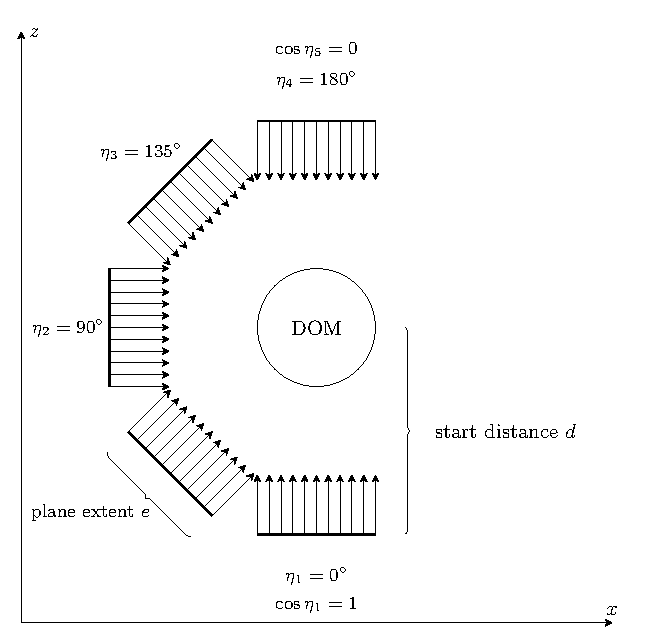
\includegraphics[width=0.9\textwidth]{img/angular-acceptance-coordinates-plane-waves-Ii2nieki}
        \caption{View from the side. Shooting photons from different polar angles.}
      \end{figure}
    \end{column}
    \begin{column}{0.5\textwidth}
      \begin{figure}
        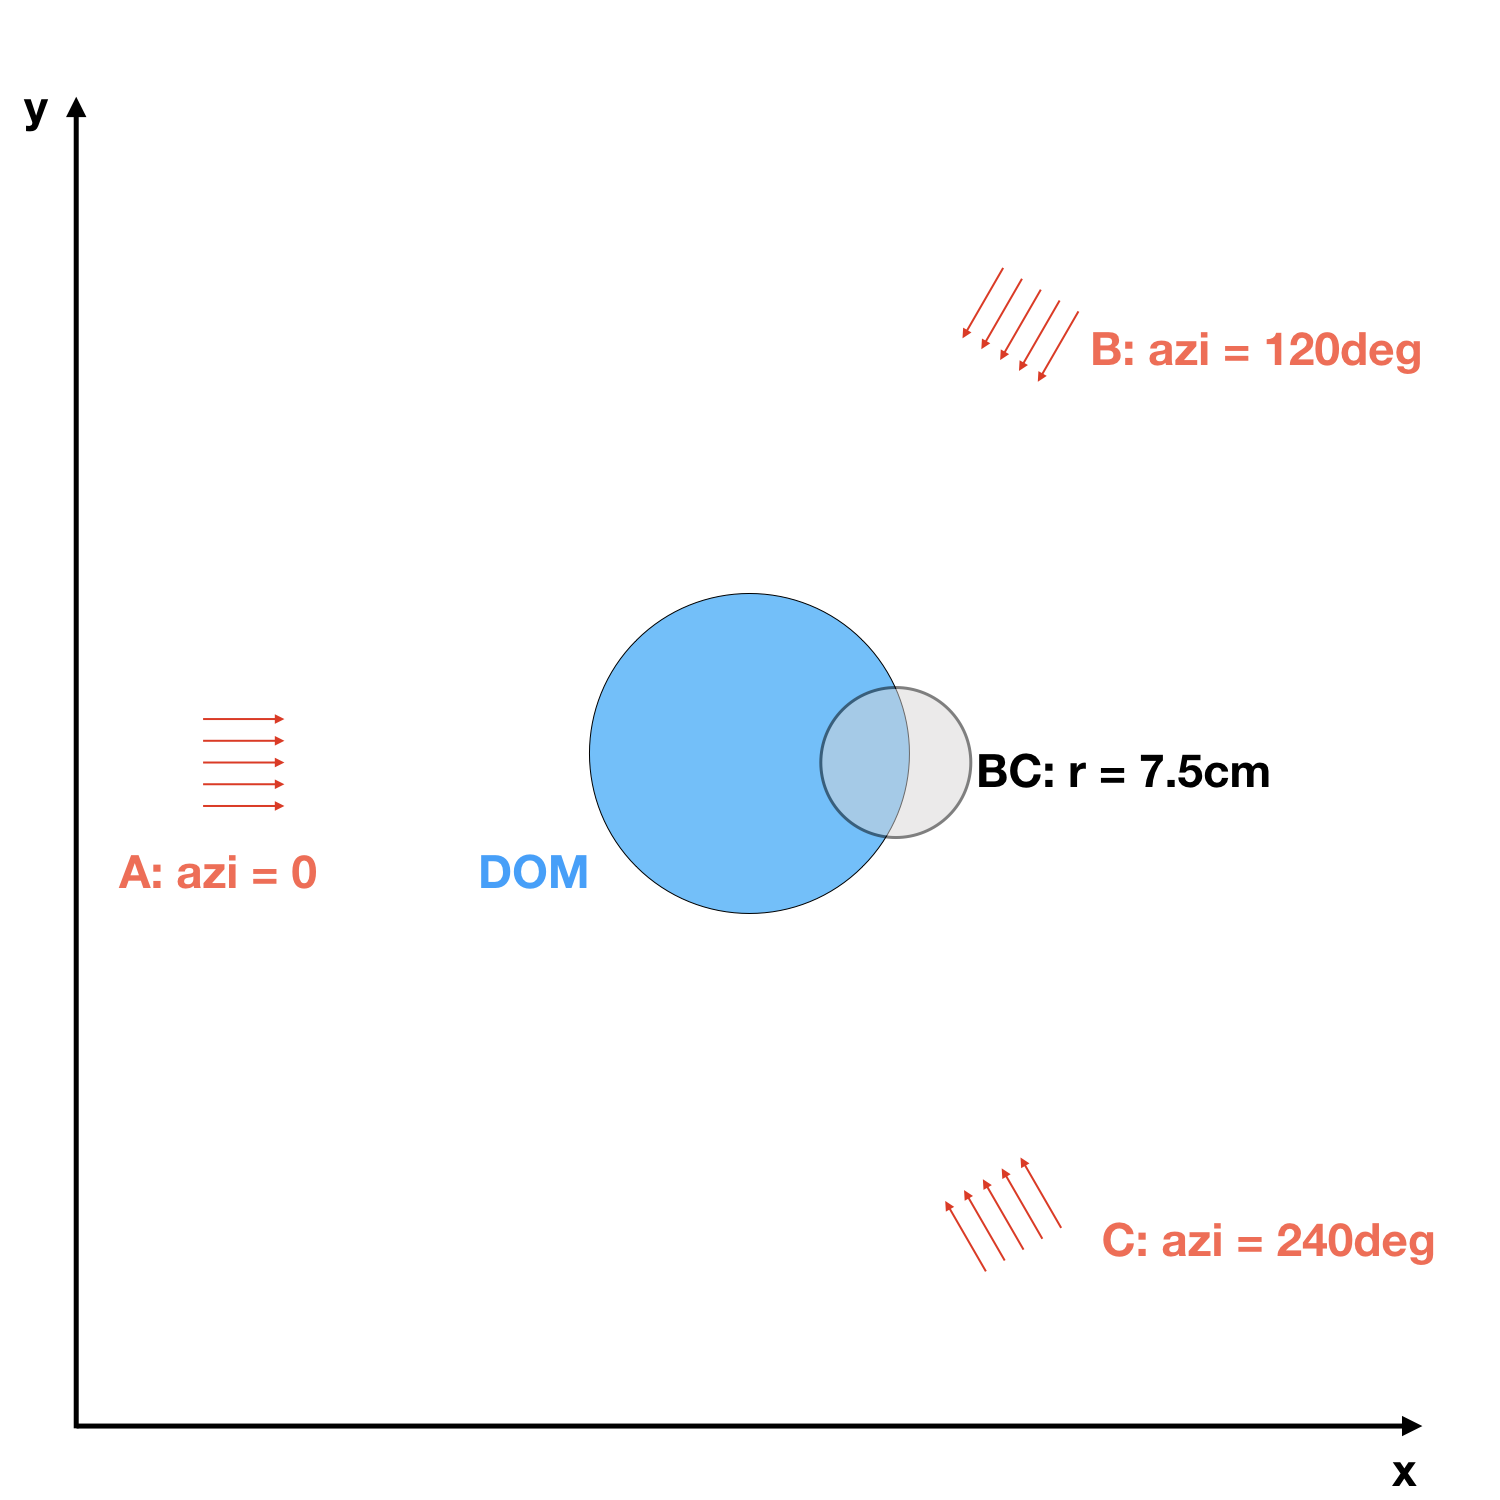
\includegraphics[width=0.9\textwidth]{img/summerscenario-003}
        \caption{View from above. Shooting photons from different azimuthal angles.}
      \end{figure}
    \end{column}
  \end{columns}
\end{frame}

\section{Simulation results}
\subsection{bubble-column radius $7.5\cm$, geometric scattering length $10\cm$}
\begin{frame}[fragile]{Simulation results}
  \begin{columns}
    \begin{column}{0.5\textwidth}
      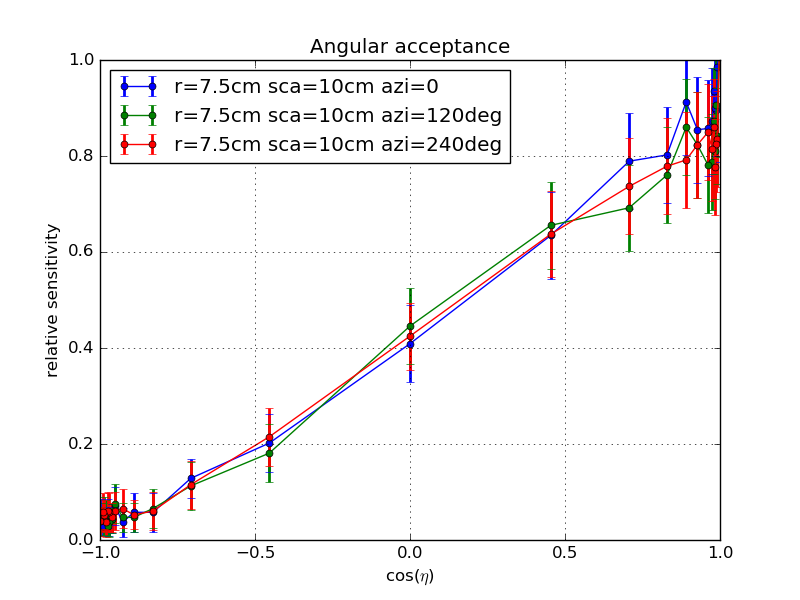
\includegraphics[width=\textwidth]{img/summer_scenario_r7-5cm_sca10cm}
    \end{column}
    \begin{column}{0.5\textwidth}
      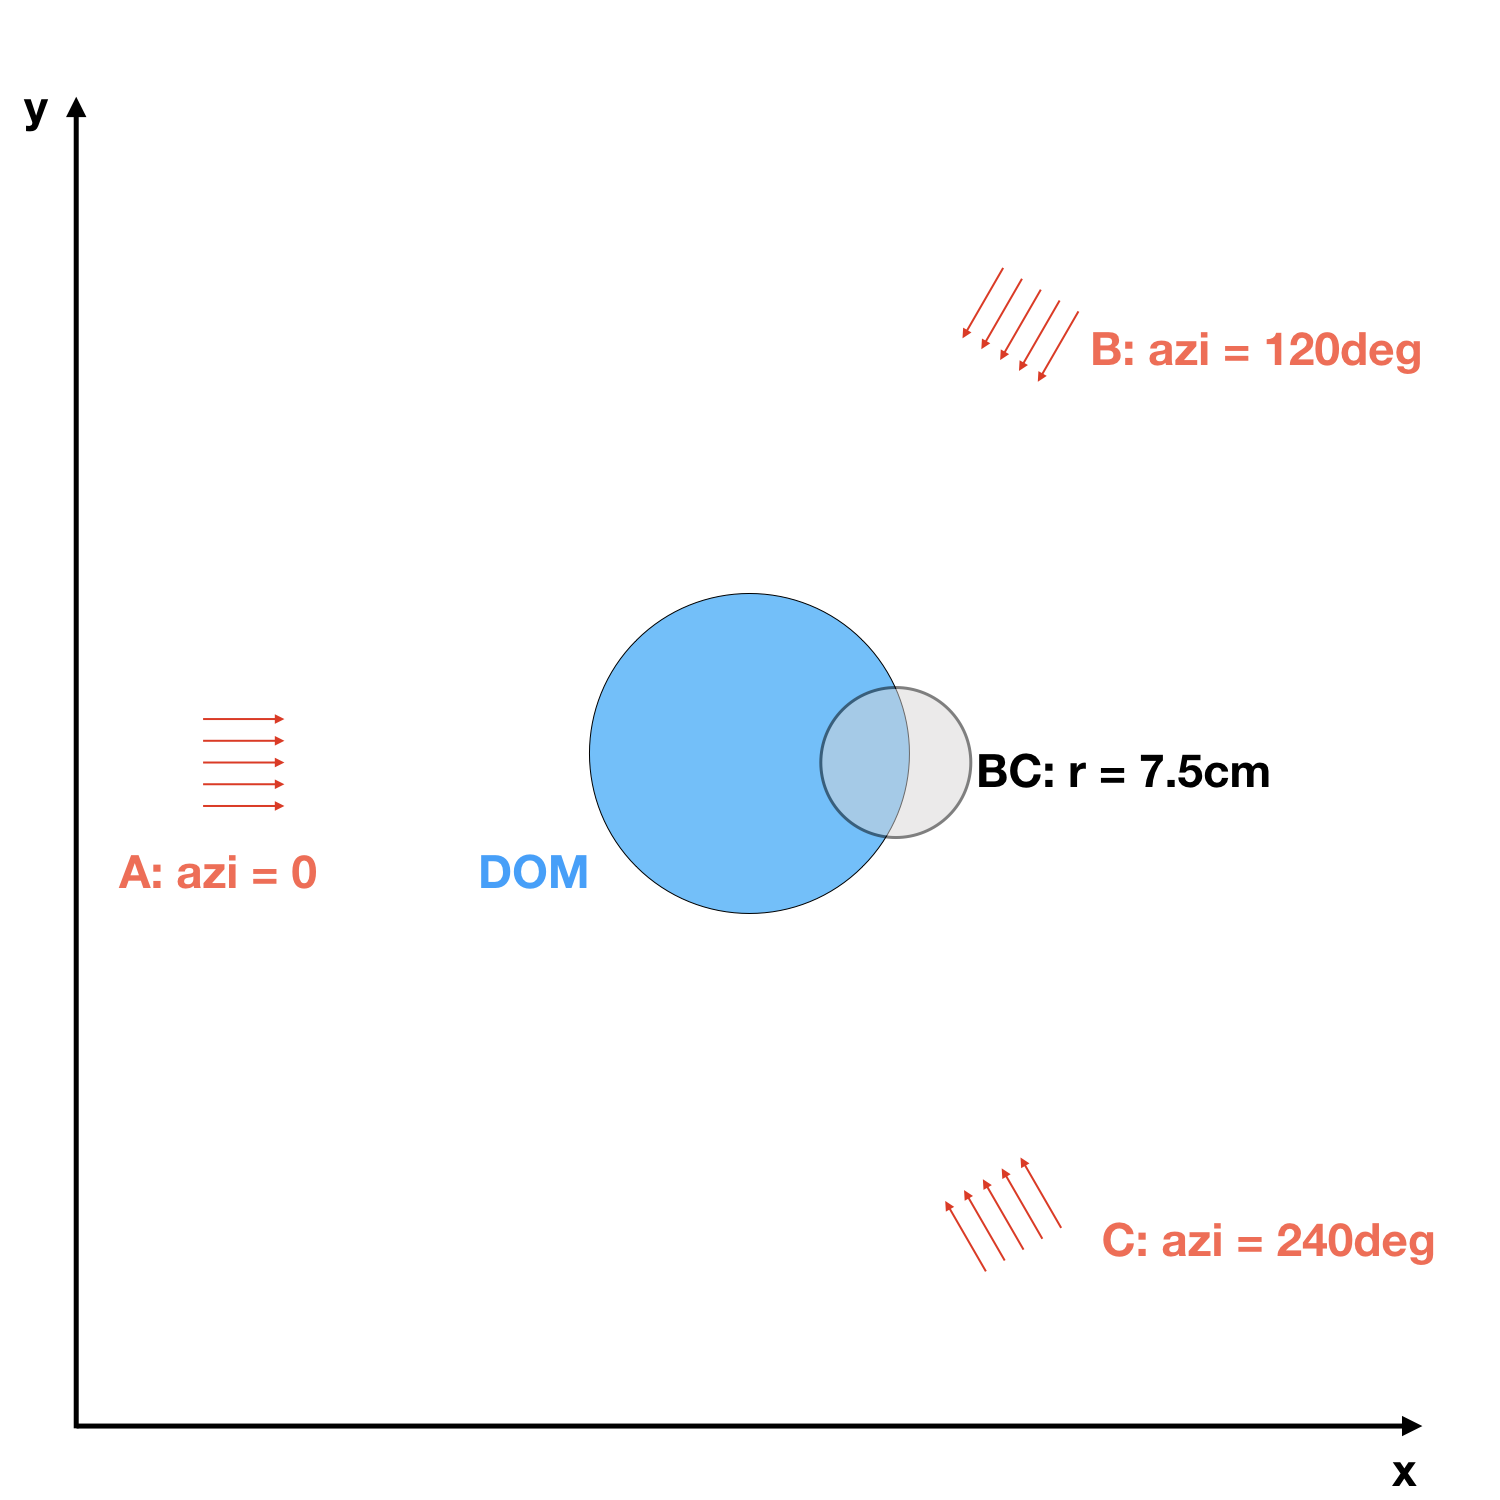
\includegraphics[width=0.8\textwidth]{img/summerscenario-003}
    \end{column}
  \end{columns}

  \tiny Total photon hit count: 12968 / 1e6

  \tiny Configuration: Starting distance $3\m$, plane-wave extent $3\m$, bubble-column geometric scattering length $10\cm$, bulk-ice geometric scattering length $130\cm$.
  \normalsize

  \begin{itemize}
    \item For lower polar angles ($\cos\eta \approx 1$), less photons should arrive from azimuths B and C as from azimuth A
      \tiny as the DOM's PMTs look downwards and photons from B and C are more likely to cross the bubble-column cylinder. \normalsize
    \item From azimuths B and C, the same number of photons should arrive \tiny due to the symmetry of the scenario (right image). \normalsize
  \end{itemize}
\end{frame}

\subsection{bubble-column radius $15\cm$, geometric scattering length $10\cm$}
\begin{frame}[fragile]{Simulation results}
  \begin{columns}
    \begin{column}{0.5\textwidth}
      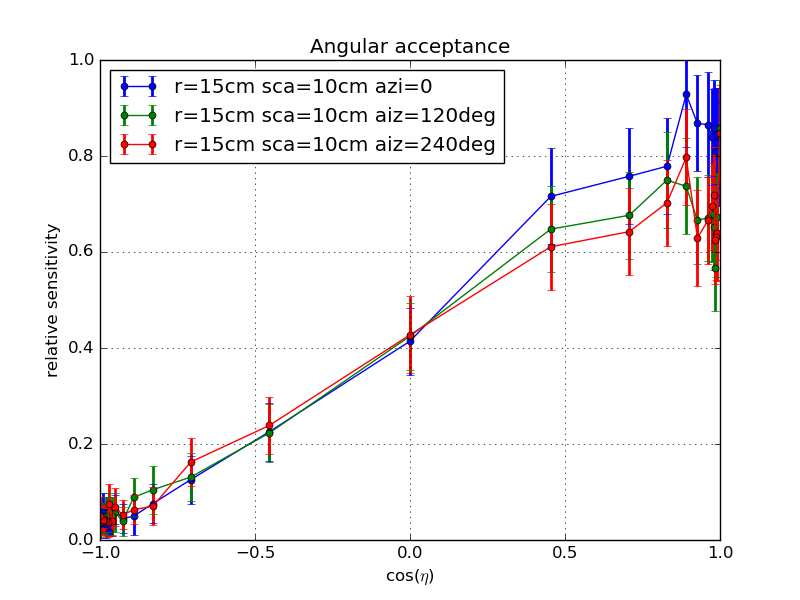
\includegraphics[width=\textwidth]{img/summer_scenario_r15cm_sca10cm}
    \end{column}
    \begin{column}{0.5\textwidth}
      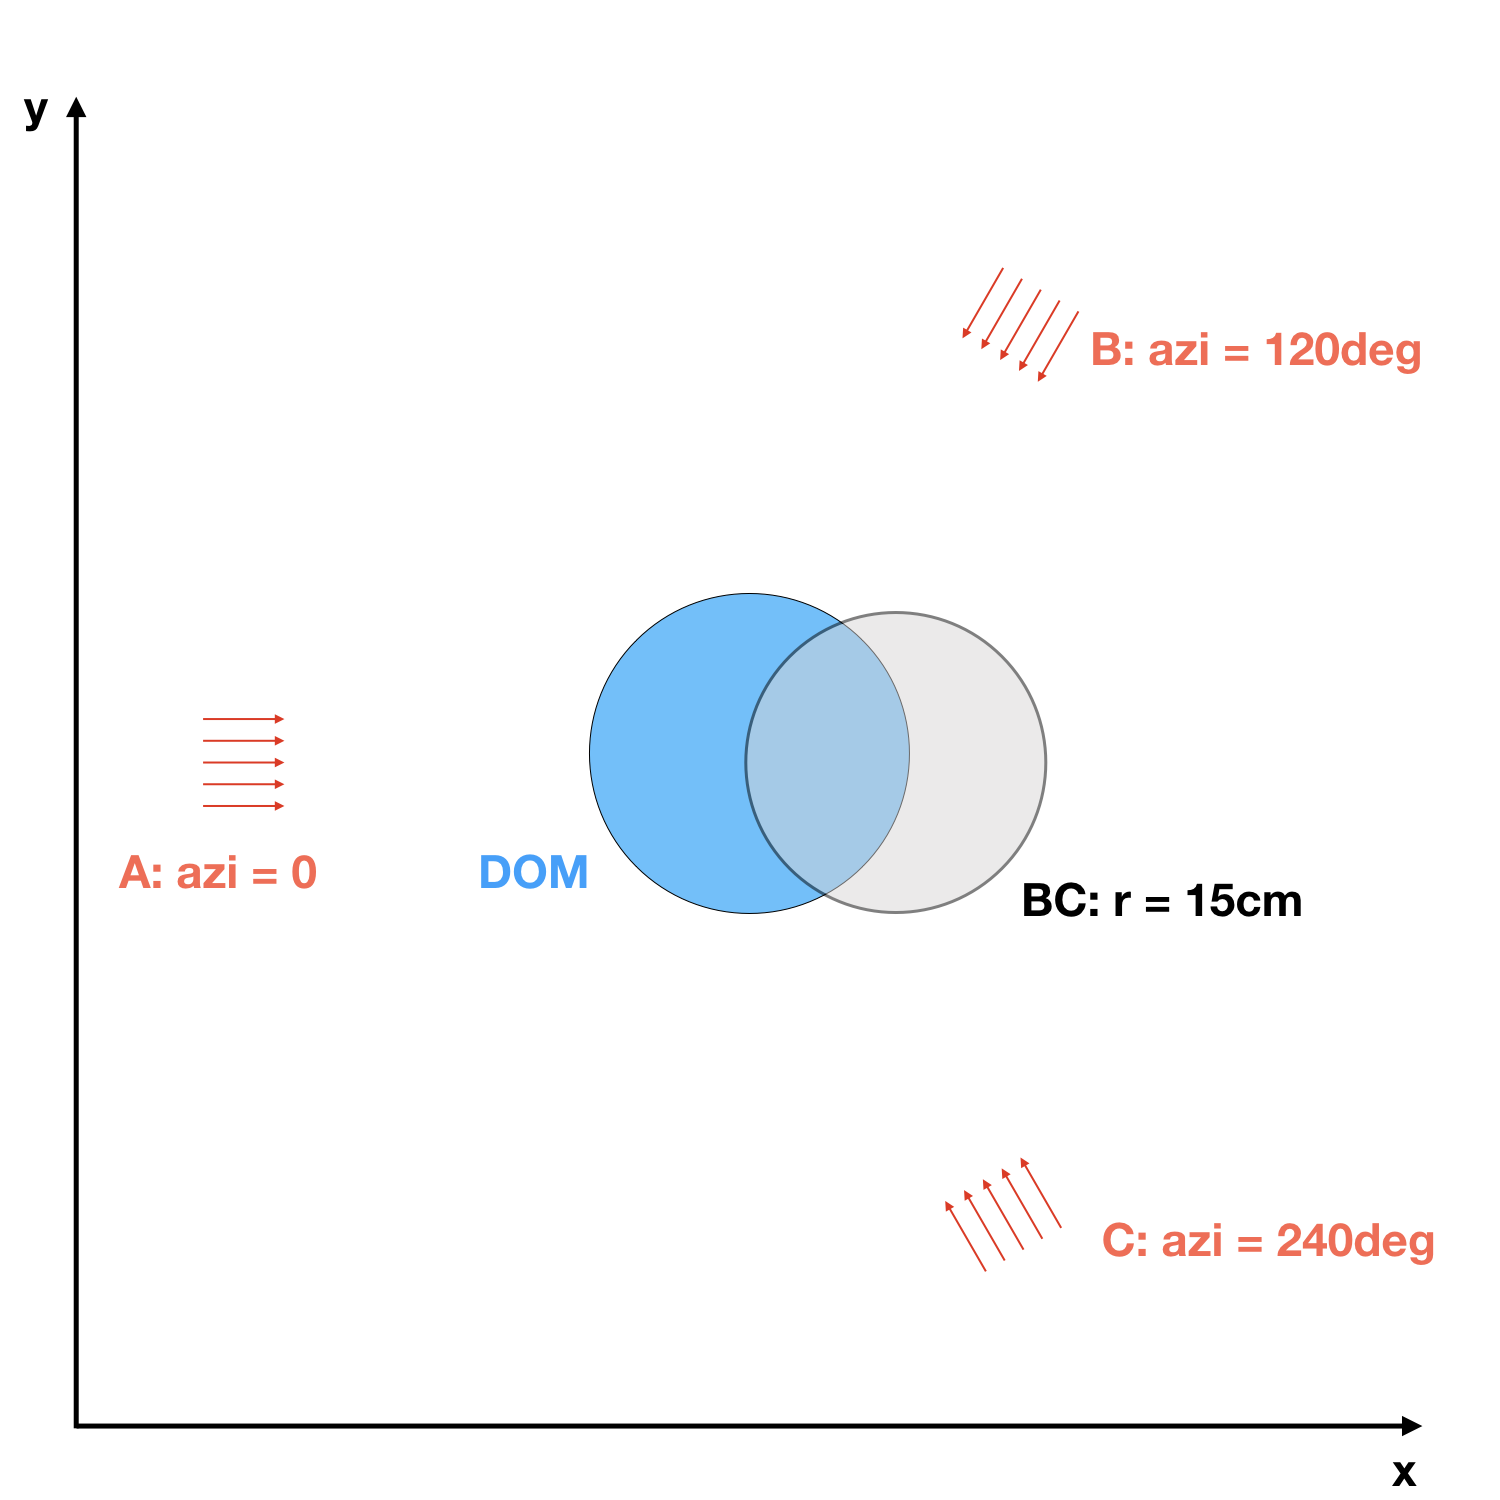
\includegraphics[width=0.8\textwidth]{img/summerscenario-004}
    \end{column}
  \end{columns}

  \tiny Total photon hit count: 11600 / 1e6

  \tiny Configuration: Starting distance $3\m$, plane-wave extent $3\m$, bubble-column geometric scattering length $10\cm$, bulk-ice geometric scattering length $130\cm$.
  \normalsize

  \begin{itemize}
    \item For a larger bubble column with same scattering lenght, the effect should increase. \checkmark
  \end{itemize}
\end{frame}

\subsection{bubble-column radius $15\cm$, geometric scattering length $70\cm$}
\begin{frame}[fragile]{Simulation results}
  \begin{columns}
    \begin{column}{0.5\textwidth}
      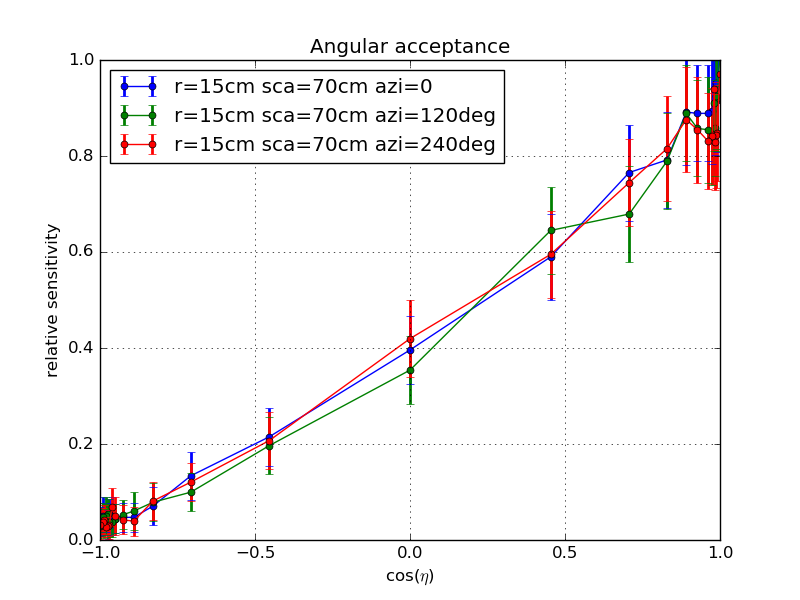
\includegraphics[width=\textwidth]{img/summer_scenario_r15cm_sca70cm}
    \end{column}
    \begin{column}{0.5\textwidth}
      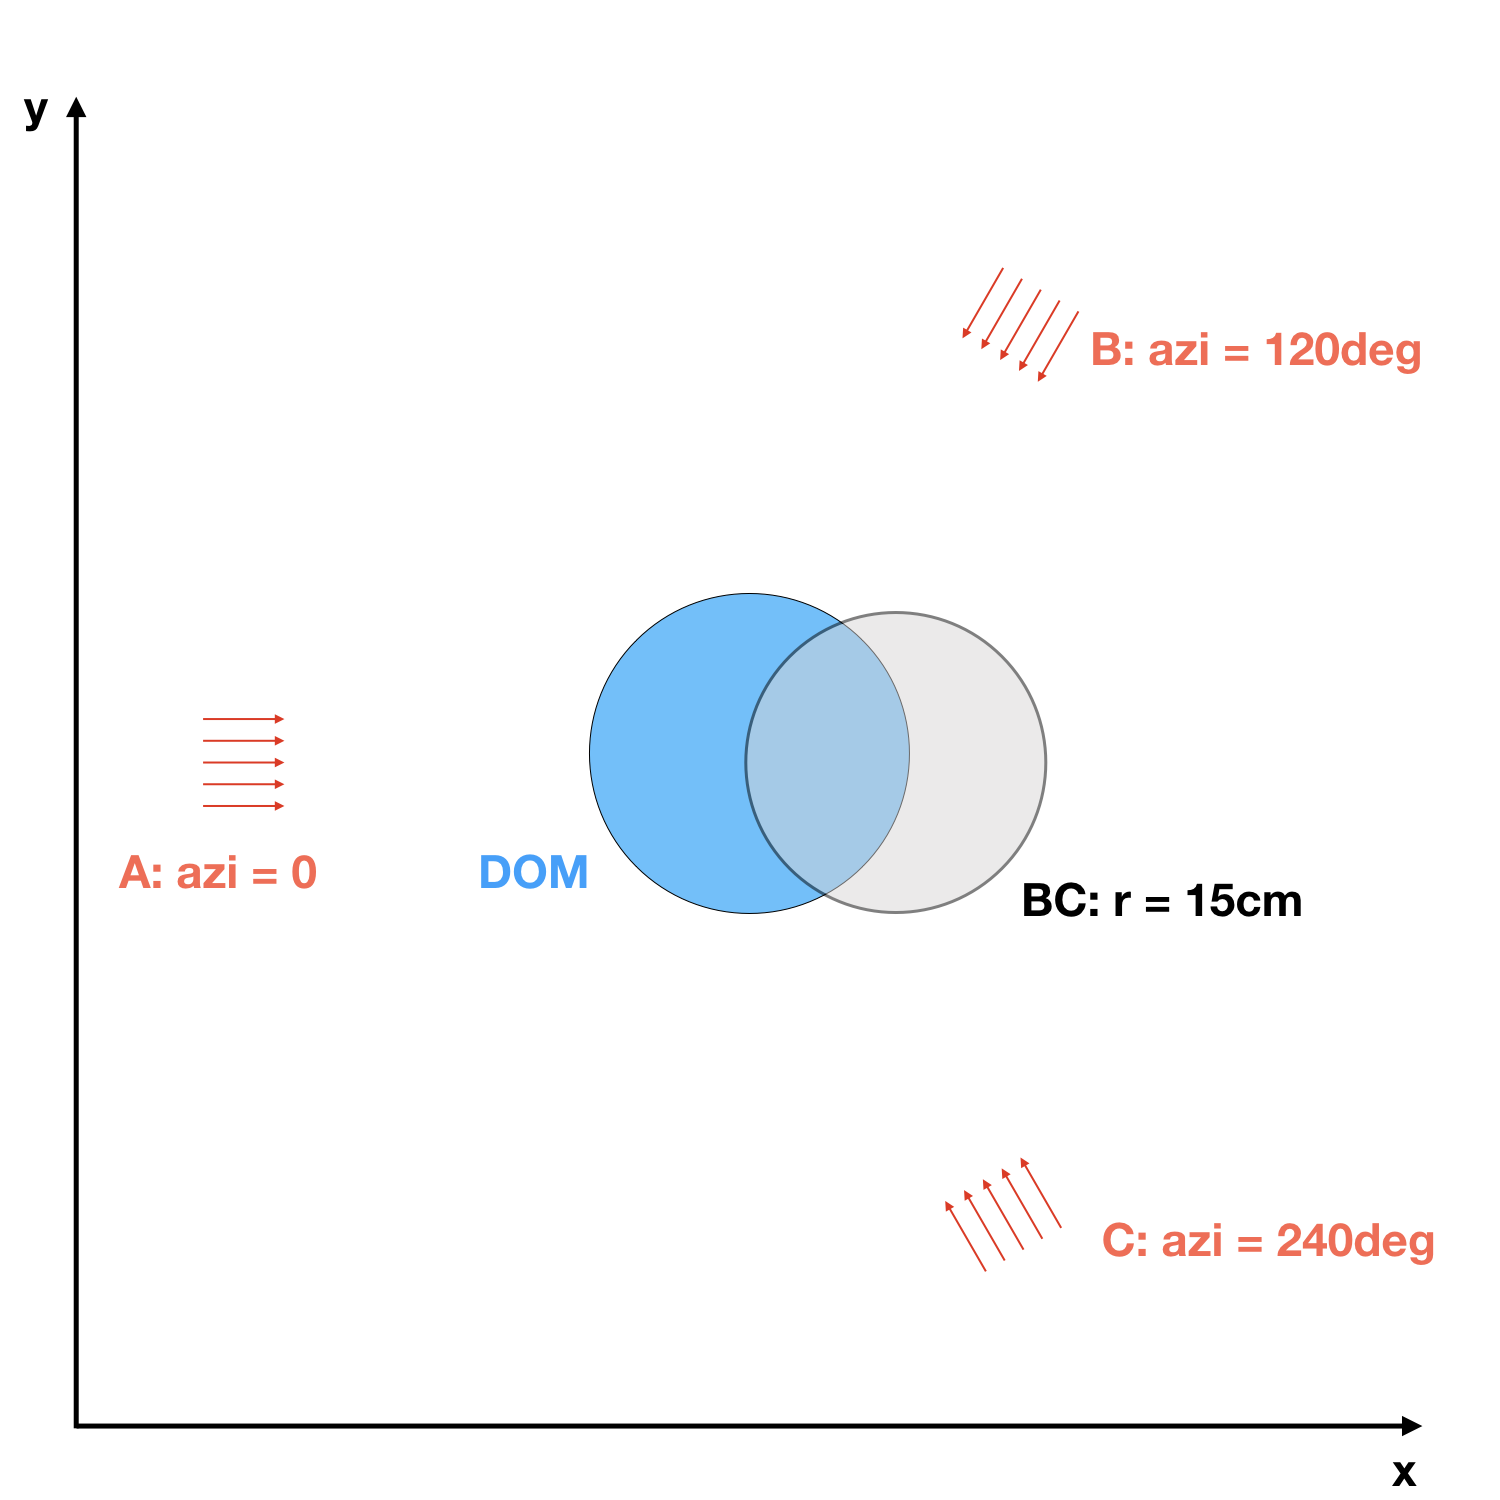
\includegraphics[width=0.8\textwidth]{img/summerscenario-004}
    \end{column}
  \end{columns}

  \tiny Total photon hit count: 13115 / 1e6

  \tiny Configuration: Starting distance $3\m$, plane-wave extent $3\m$, bubble-column geometric scattering length $70\cm$, bulk-ice geometric scattering length $130\cm$.
  \normalsize

  \begin{itemize}
    \item For a larger scattering length (weaker bubble column), the effect should decrease. \checkmark
  \end{itemize}
\end{frame}

\subsection{bubble-column radius $30\cm$, geometric scattering length $70\cm$}
\begin{frame}[fragile]{Simulation results}
  \begin{columns}
    \begin{column}{0.5\textwidth}
      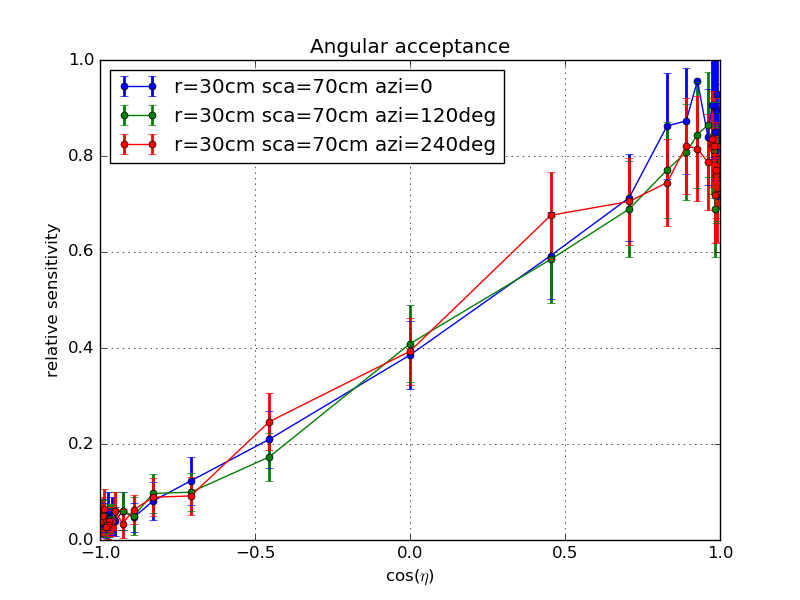
\includegraphics[width=\textwidth]{img/summer_scenario_r30cm_sca70cm}
    \end{column}
    \begin{column}{0.5\textwidth}
      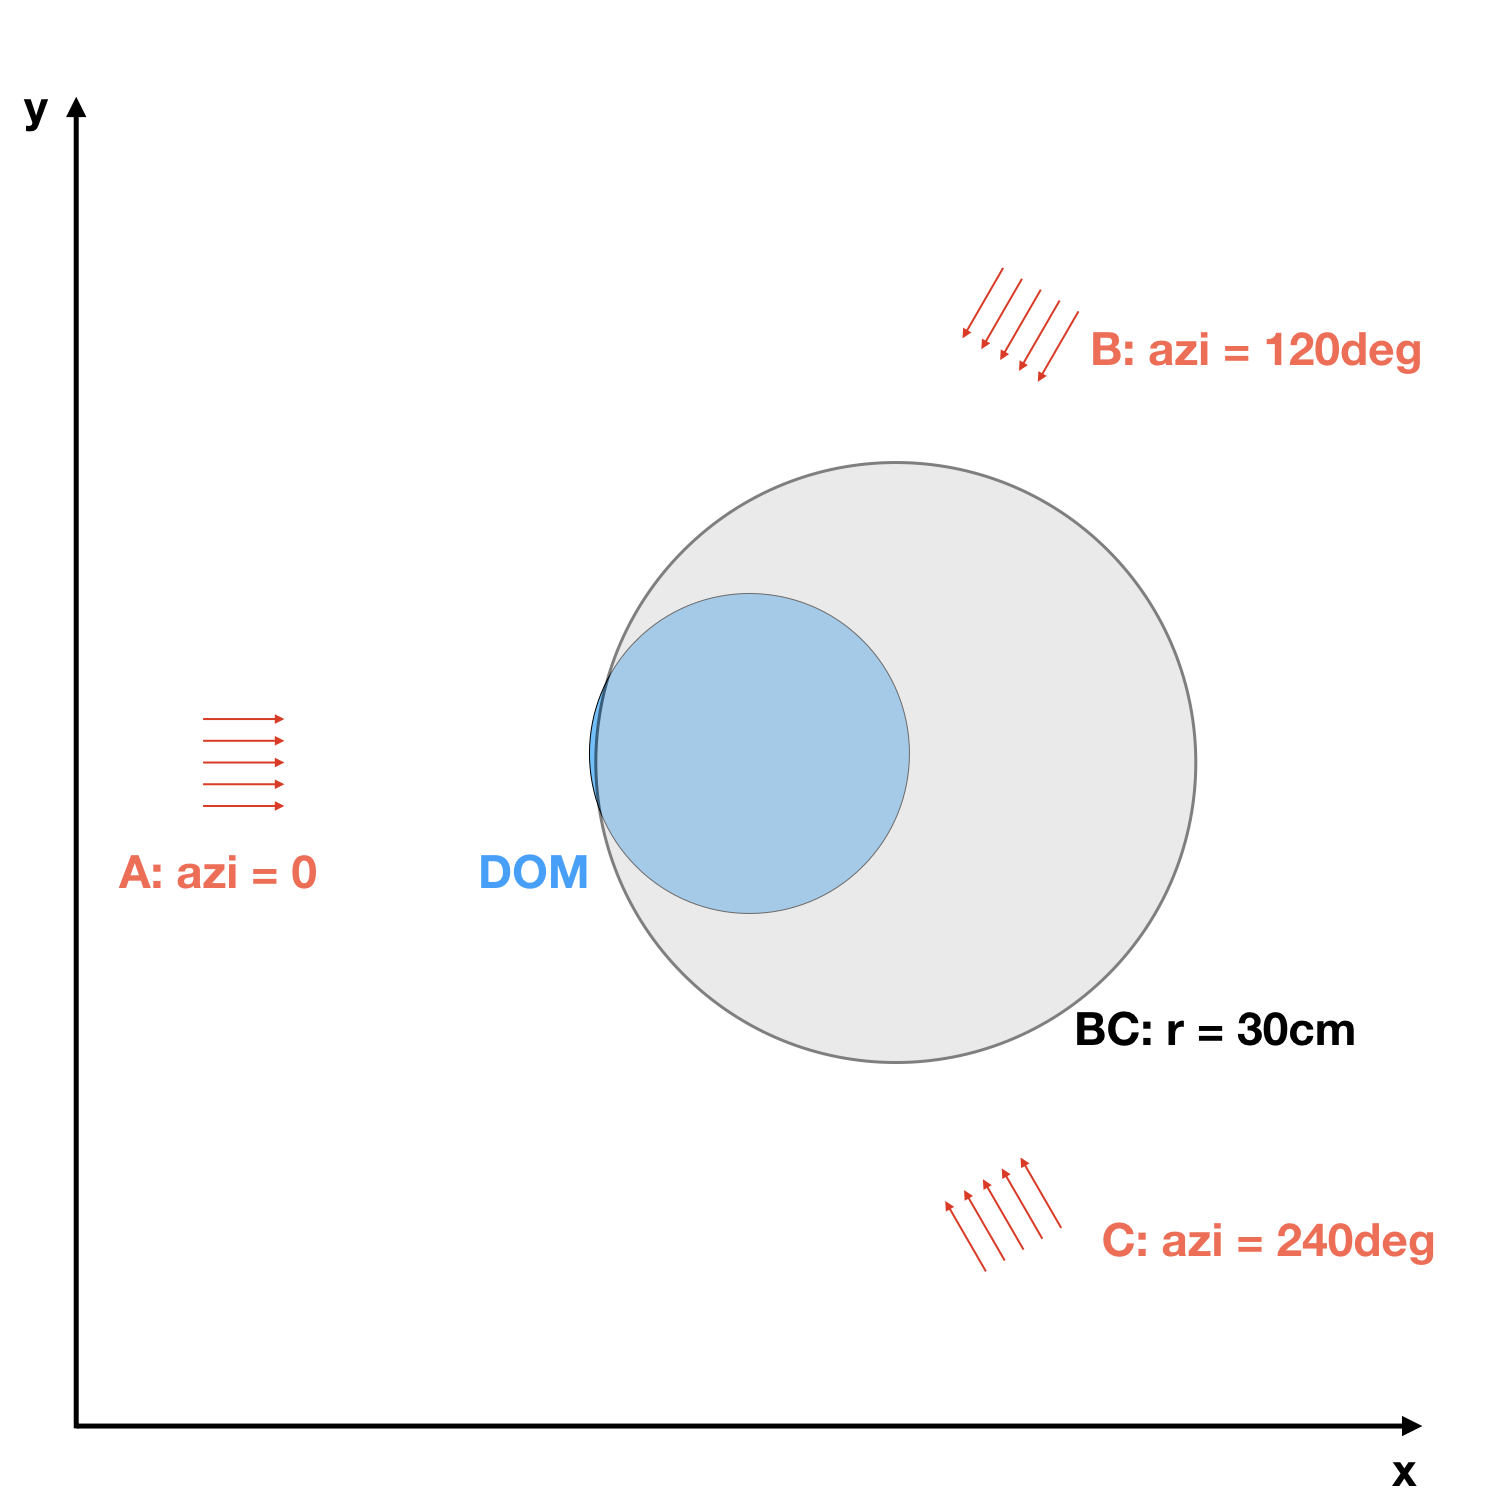
\includegraphics[width=0.8\textwidth]{img/summerscenario-005}
    \end{column}
  \end{columns}

  \tiny Total photon hit count: 12339 / 1e6

  \tiny Configuration: Starting distance $3\m$, plane-wave extent $3\m$, bubble-column geometric scattering length $70\cm$, bulk-ice geometric scattering length $130\cm$.
  \normalsize

  \begin{itemize}
    \item For a larger bubble column, the effect should increase.
    \item Less photons should arrive in total \tiny as the whole DOM is now shielded by the hole ice. \normalsize \checkmark
  \end{itemize}
\end{frame}

\subsection{Compare different bubble columns for same angle}
\begin{frame}[fragile]{Simulation results}
  \begin{columns}
    \begin{column}{0.5\textwidth}
      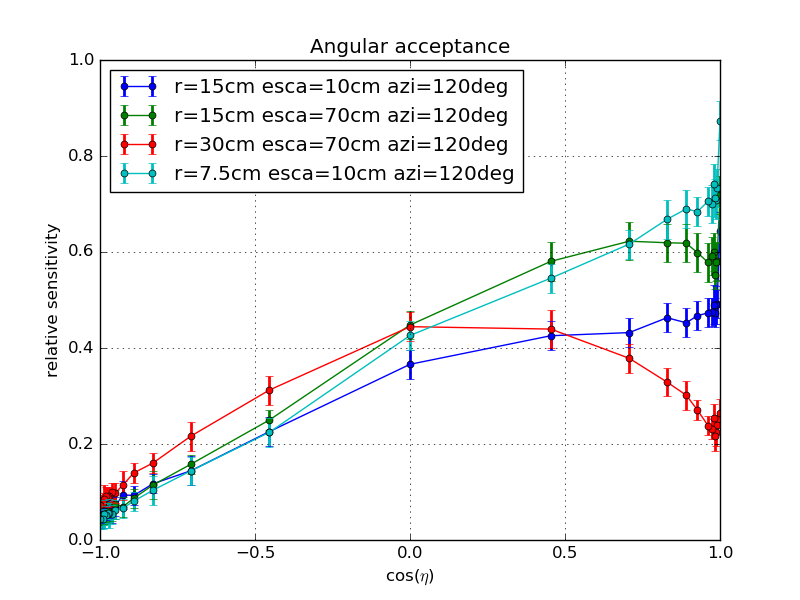
\includegraphics[width=\textwidth]{img/summer_scenario_azi120deg}
    \end{column}
    \begin{column}{0.5\textwidth}
      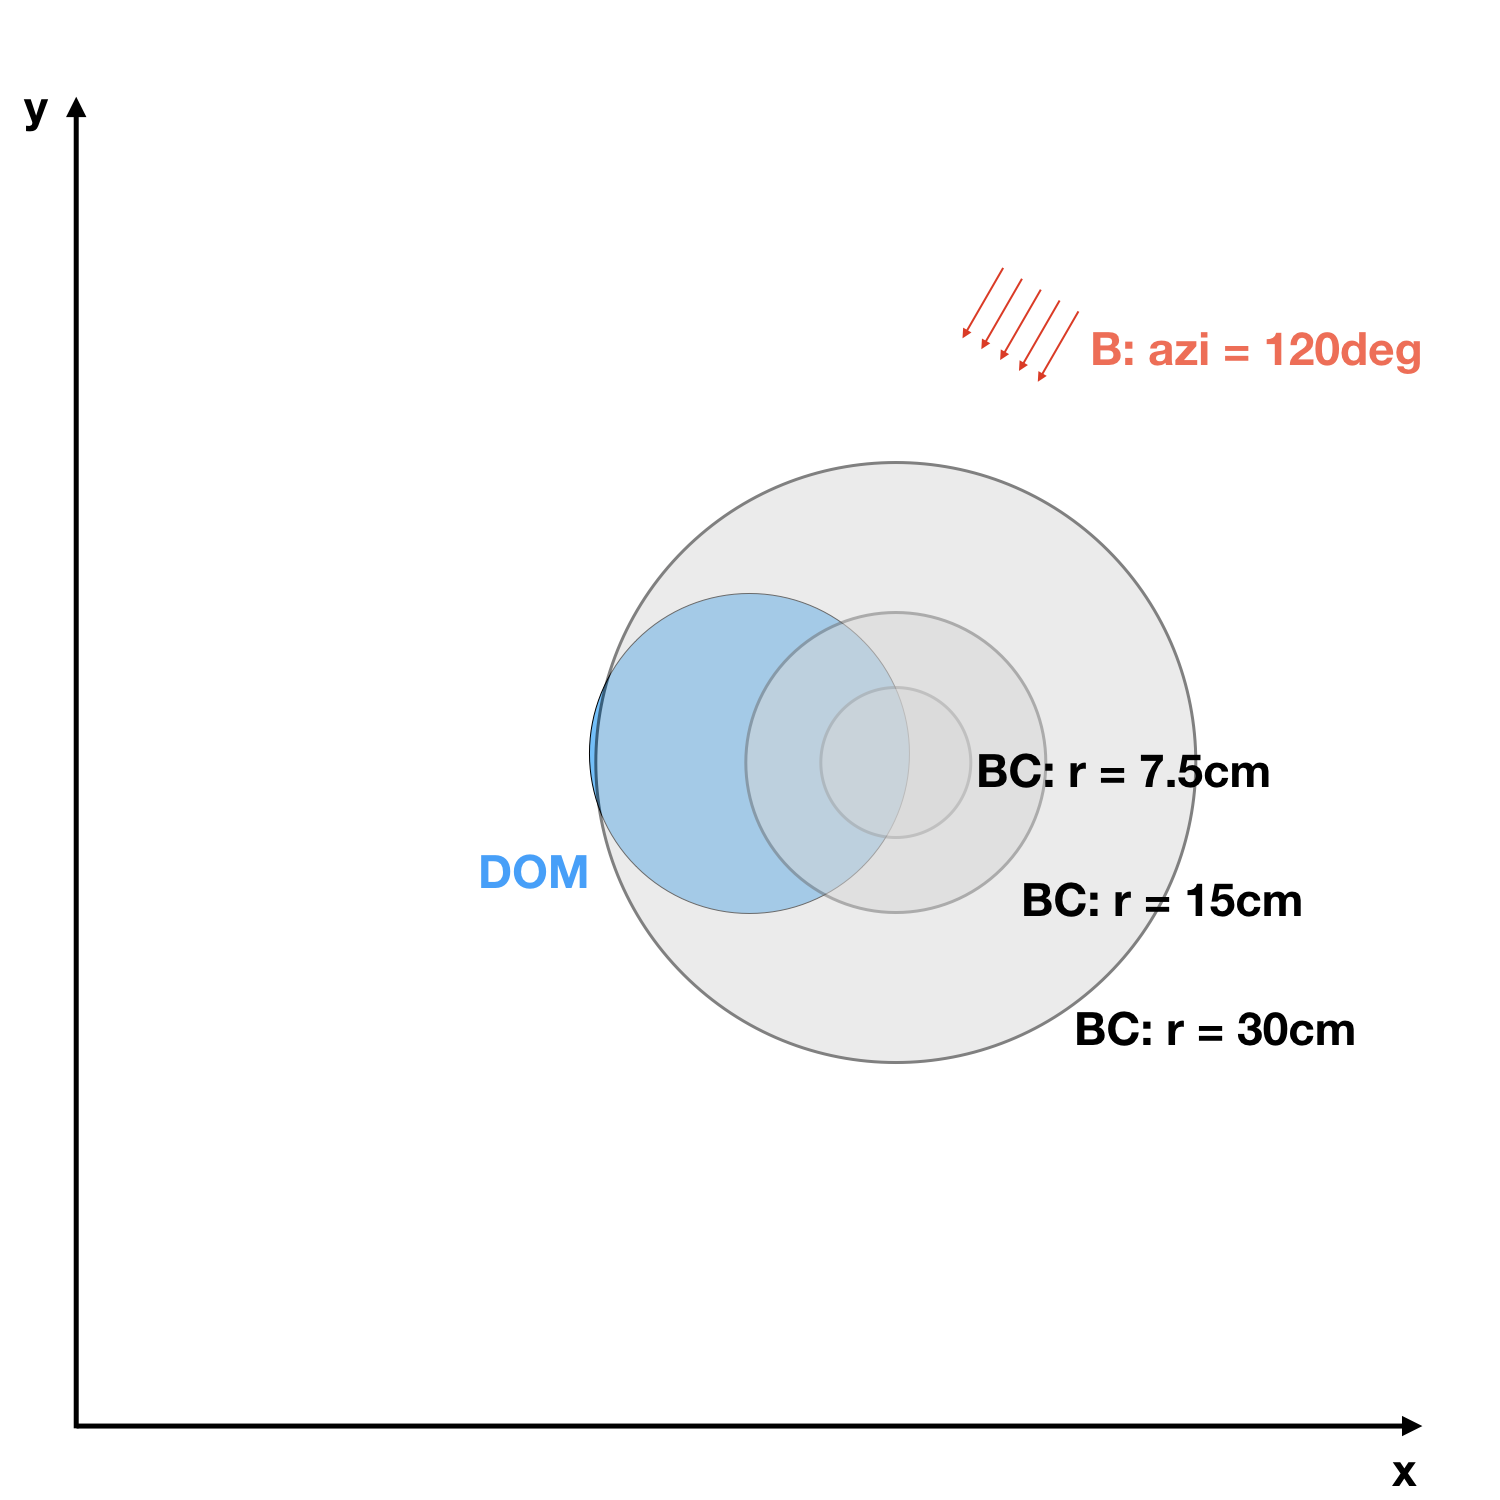
\includegraphics[width=0.8\textwidth]{img/summerscenario-006}
    \end{column}
  \end{columns}

  \tiny Configuration: Starting distance $3\m$, plane-wave extent $3\m$, bulk-ice geometric scattering length $130\cm$.
  \normalsize

  \begin{itemize}
    \item Comparing different bubble columns for the same direction of incoming photons.
    \item For a stronger or larger bubble column, the effect should increase.
  \end{itemize}
\end{frame}

\section{}
\begin{frame}[fragile]{Thanks for your attention!}
  \begin{center}
  Any input you might have is welcome: \\ \vspace{0.3cm}

  \url{https://github.com/fiedl/hole-ice-study/issues/117} \\ \vspace{0.1cm}

  Slack:
  \href{https://icecube-spno.slack.com/messages/U0BJE7Z7T}{\texttt{@sblot}}
  \&
  \href{https://icecube-spno.slack.com/messages/@U092MBFU2}{\texttt{@fiedl}}

  \vspace{1.5cm}

  \includegraphics[height=3cm]{img/summerscenario-steamshovel}

  YouTube video of the simulation:

  \url{https://www.youtube.com/watch?v=M_QGNdGG9Ew}

  \end{center}
\end{frame}
%
% \subsection{Algorithm comparison}
%   %!TEX TS-program = ../make.zsh

\begin{frame}[fragile]{Two hole-ice algorithms}

  \begin{tabelle}{l|L|L}
    & \textbf{Algorithm (a)} & \textbf{Algorithm (b)} \\
    \hline
    Approach
      & Leave clsim medium propagation as it is and add \textbf{hole-ice effects as correction} afterwards
      & Unify clsim medium propagation through layers and hole ice: Treat them as \textbf{generic medium changes} \\
    Hole-ice properties
      & defined relative to bulk-ice properties
      & defined absolute \\
    Pros
      &
        \begin{itemize}
          \item[+] Small surface area of hole-ice code, i.e. well testable through unit tests
          \item[+] Standard clsim almost untouched
        \end{itemize}
      &
        \begin{itemize}
          \item[+] Supports nested cylinders and cables
        \end{itemize}
      \\
    Cons
      &
        \begin{itemize}
          \item[--] Current understanding of hole-ice suggests defining hole-ice properties absolute rather than relative
        \end{itemize}
      &
        \begin{itemize}
          \item[--] Needed rewrite of clsim's medium-propagation code
          \item[--] Ice tilt and ice anisotropy not re-implemented, yet
        \end{itemize}
  \end{tabelle}

\end{frame}
%
\subsection{Comparison to ppc simulation}
  %!TEX TS-program = ../make.zsh

\begin{frame}{Comparison to ppc simulation}

  \begin{center}
  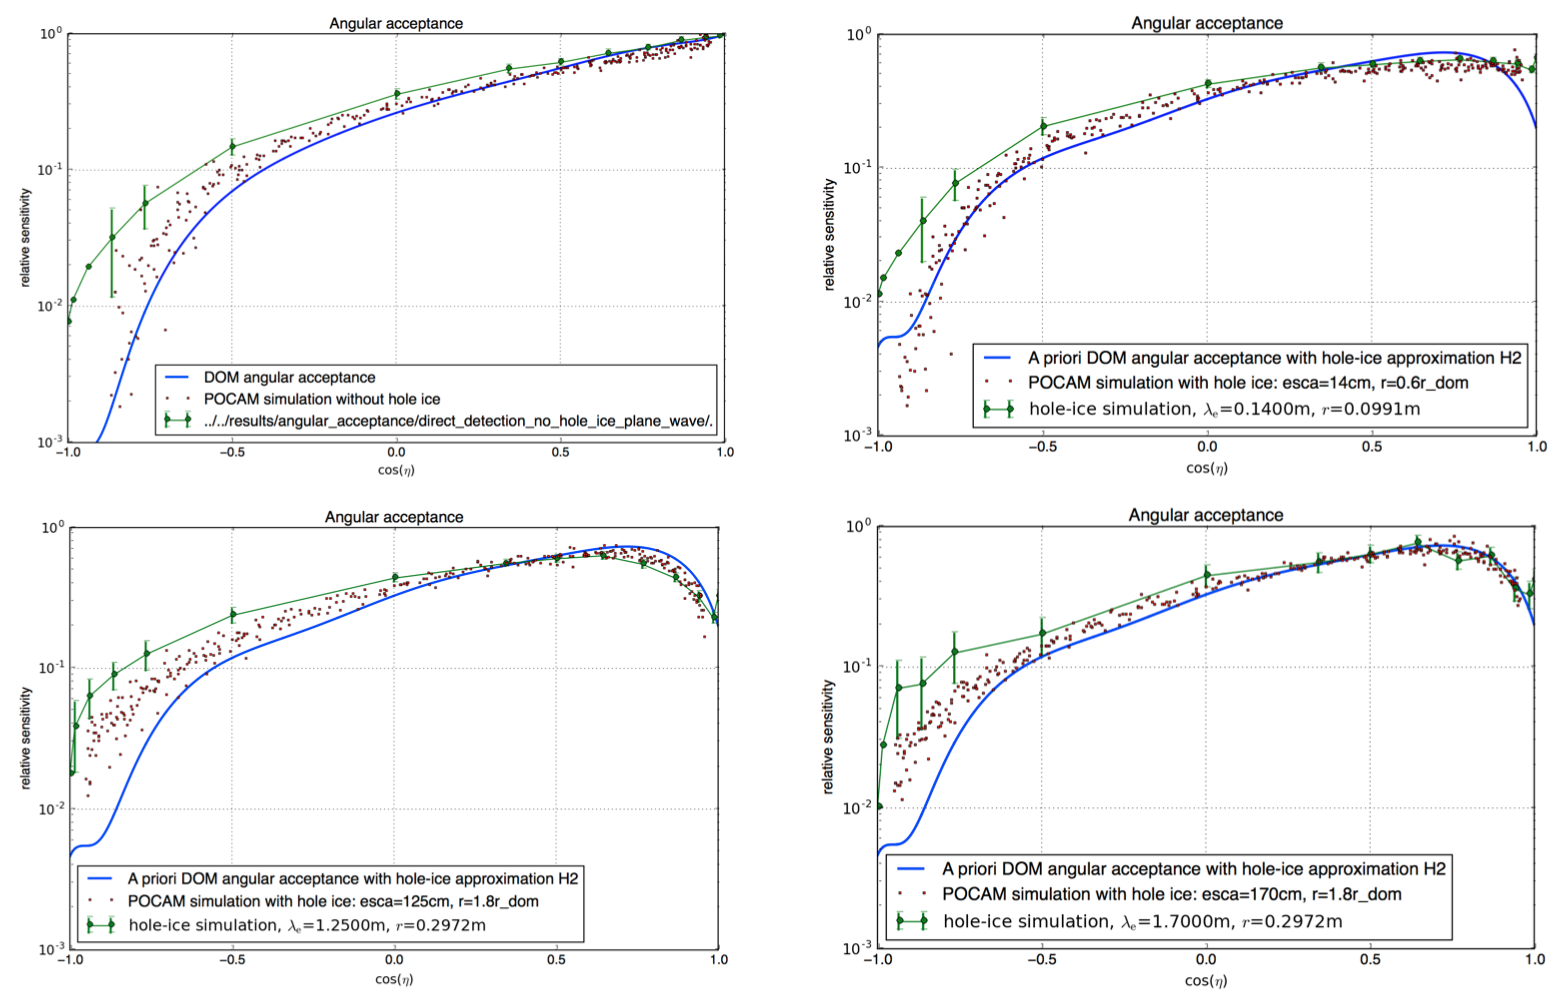
\includegraphics[height=0.8\textheight]{img/ppc-pocam}
  \end{center}

  \source{\url{https://github.com/fiedl/hole-ice-study/issues/4}, POCAM ppc data source: Resconi, Rongen, Krings: The Precision Optical CAlibration Module for IceCube-Gen2: First Prototype, 2017.}

\end{frame}

\subsection{Comparison to H2 hole-ice model}
  %!TEX TS-program = ../make.zsh

\begin{frame}[fragile]{Comparison to H2 hole-ice model}
  \image{h2_comparison}
  \source{\url{https://github.com/fiedl/hole-ice-study/issues/80}. \her{H2 curve source}: IceCube Collaboration et al. Measurement of South Pole ice transparency with the IceCube LED calibration system. 2013. \her{H2 parameter source}: Albrecht Karle. Hole Ice Studies with YAG. \url{http://icecube.berkeley.edu/kurt/interstring/hole-ice/yak.html}. 1998.}
\end{frame}
\subsection{Comparison of parameters from calibration measurements}
  %!TEX TS-program = ../make.zsh

\begin{frame}[fragile]{Comparison of parameters from calibration measurements}

  % \begin{columns}
  %   \begin{column}{0.5\textwidth}
  %     \image{angular-acceptance-karle-h2-xaeg2Mee}
  %
  %     \image{angular-acceptance-splicehd-ku3Zie8z}
  %   \end{column}
  %   \begin{column}{0.5\textwidth}
  %     \image{angular-acceptance-dard-eePai1sh}
  %
  %   \end{column}
  % \end{columns}

  \begin{center}
    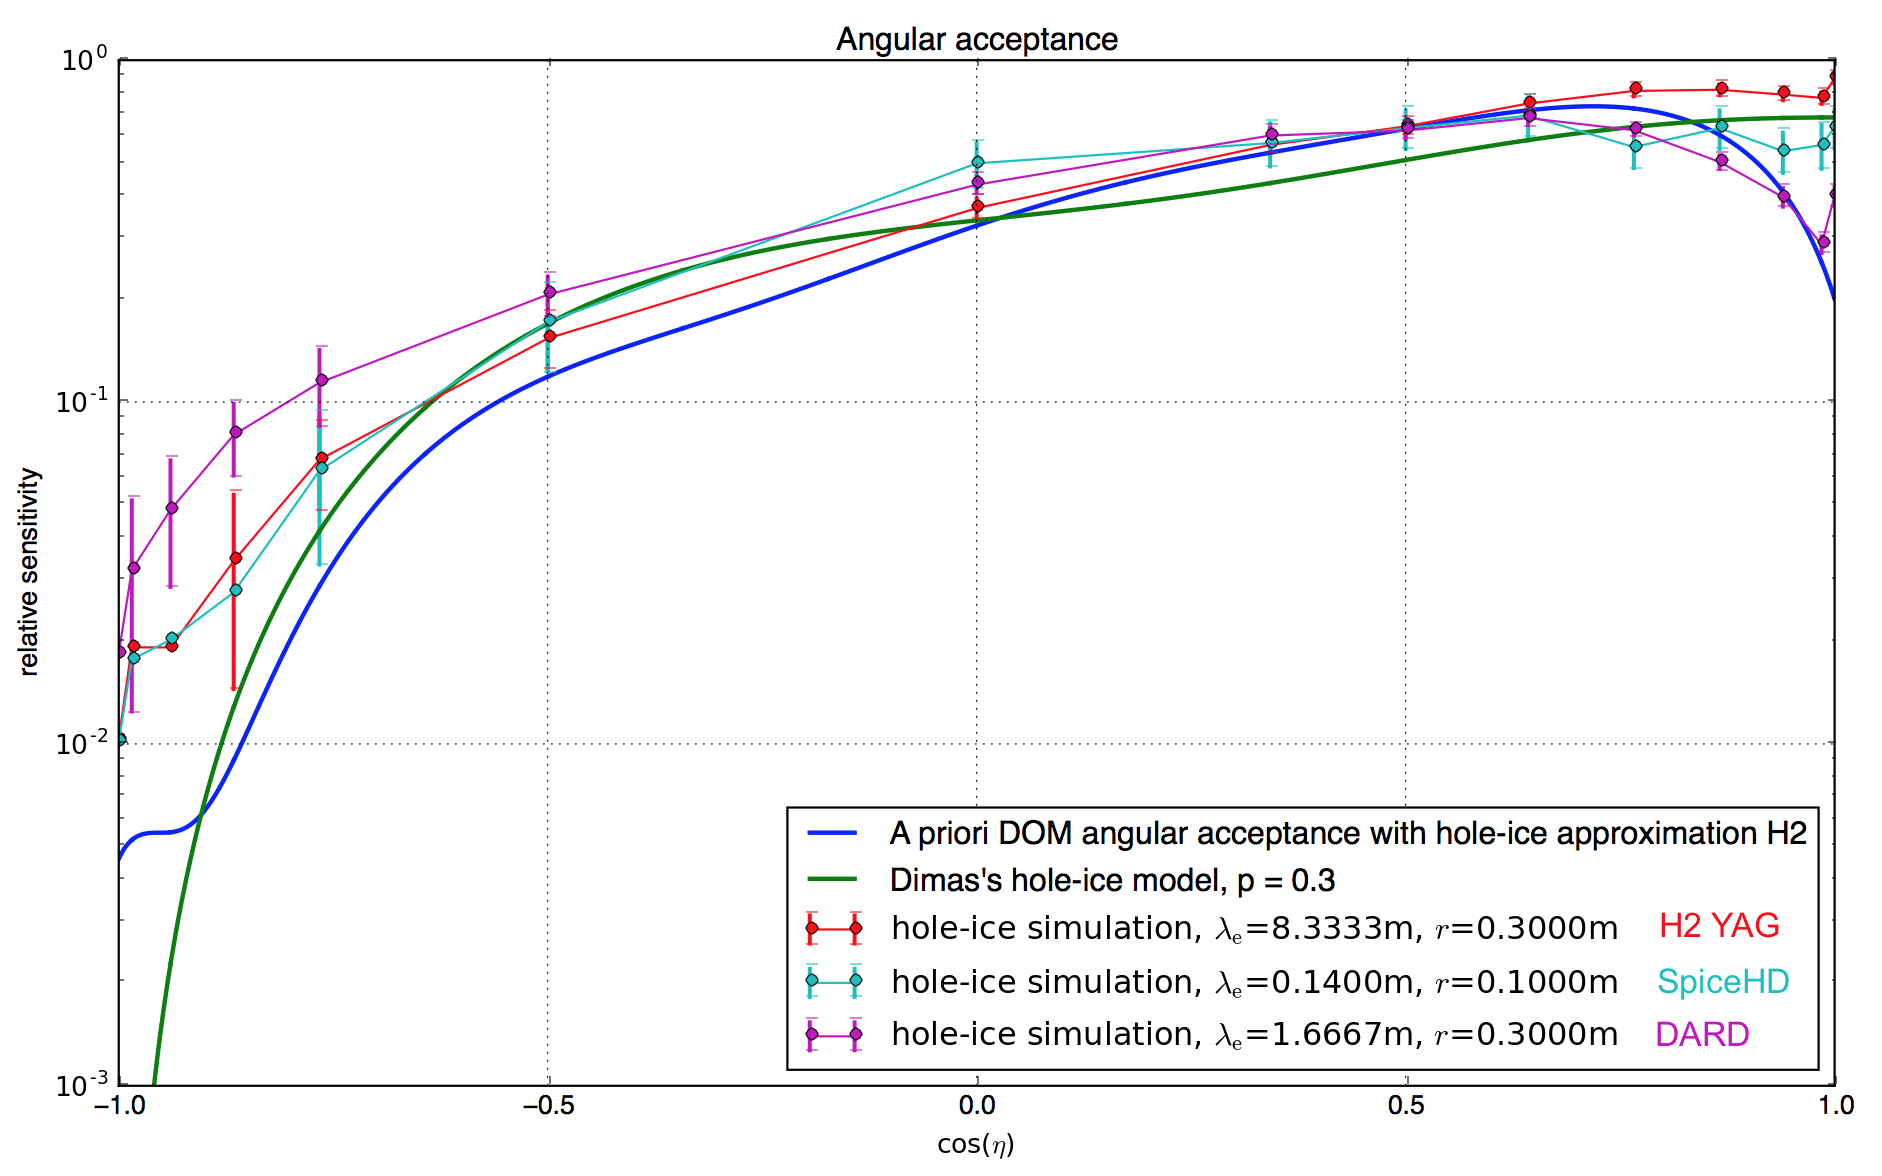
\includegraphics[height=.7\textheight]{img/angular-acceptance-calibration-measurements}
  \end{center}

  \vtiny{%
    \her{Source}:
    \url{https://github.com/fiedl/hole-ice-study/issues/104}
    \her{H2 YAG}: \url{https://github.com/fiedl/hole-ice-study/issues/80}. Karle, Hole Ice Studies with YAG, \url{http://icecube.berkeley.edu/kurt/interstring/hole-ice/yak.html}, 1998.
    \her{SpiceHD}: \url{https://github.com/fiedl/hole-ice-study/issues/87}. Rongen, Status and future of SpiceHD and DARD, Calibration Workshop August 2017.
    \her{DARD}: \url{https://github.com/fiedl/hole-ice-study/issues/105}. Rongen, Measuring the optical properties of IceCube drill holes, 2016. Rongen, DARD Update, Calibration Call 2015-11-06.
  }

\end{frame}

\end{document}